
% load the document class KOMA-Script Report
\documentclass[	
		a4paper,			% Papierformat waehlen
		11pt,				% Schriftgroesse
%		draft,				% Randueberschreitungen werden schwarz markiert
%		DIV13,				% Unterteilung des Blatts in DIVxx - xx Teile              OBSOLETE
						% Je kleiner die Zahl umso groesser die Raender
						% Um Optimale Anpassung zu erhalten : DIVcalc + \typearea...
%		BCOR5mm,			% Bindekorrektur BCORXmm - Xmm breit                       OBSOLETE
		%pointlessnumbers,		% KEIN ZWEITER PUNKT IN DER NUMMERIERUNG DER ÜBERSCHRIFTET 2.2 statt 2.2.	
%
%      KOPF/FUSSZEILE
%		headinclude,			% Head gehoert mit zum Textblock/auskommentiert im Seitenrand
		headsepline,			% Trennlinie zwischen Kopf und Text, schaltet automatisch 
						% headinclude mit ein
%		footinclude,			% wie Head nur Foot
%		footsepline,			% wie headsepline
%
%      LAYOUTPARAMETER
%		twocolumn,			% Zweispaltige Texte
		onecolumn,			% Einspaltig
%		twoside,			% Zweiseitiger Druck re -li sind gespiegelt vom Satzspiegel
		oneside,			% Einseitig
%		openright,			% Sollte bei zweiseitigem Druck eignestellt werden
%		cleardoublestandard		% Alles fuer 2Seitige mit openright: Kolumnentitel linke Seite
%		cleardoubleplain		% nur Seitenzahlen linke Seite
%		cleardoubleempty		% linke Seite ganz leer
%		chapterprefix,			% Kapitel wir zu beginn eines Kapitels ausgegeben
%		appendixprefix,			% Anhang wird vor Kapiteln im Anhang ausgegeben
		headings=normal,		% kleine ueberschriften, oder small-, oder big-headings.
						% Standard ist Big
%
%	TABELLENEIGENSCHAFTEN
		captions=tableheading,		% Um richtigen Abstand fuer Ueberschrift zu erhalten, 
						% Ueberschrift wird genommen
%
%	VERZEICHNISEINSTELLUNGEN
%		tocleft,			% Setzt das Inhaltverzeichnis nicht eingerueckt nach links
%		liststotoc,			% Abb.- und Tab.Verzeichnisse ins Inhaltsverzeichnis
%		liststotocnumbered, 		% wie liststotoc nur mit Gliederungspunktangabe
%		bibtotoc,			% Literaturverzeichnis ins Inhaltverzeichnis
%		bibtotocnumbered,		% s.o. nur mit Gliederungsebene
%		idxtotoc,			% Eintrag ins Inhaltsverzeichnis fue Index
%		openbib,			% Veraendert aussehen des Lit.-Verzeichnisses
%	Language
%		ngerman,			% to pass as standard to all packages
]{scrreprt}

% load packages for european, espacially german users

\usepackage[T1]{fontenc}			% Schriften fuer Europaeische Zeichen passend Kodiert
\usepackage[utf8]{inputenc}        		% Eingabe von Umlauten, ss usw. - 
						% utf8: kann nicht jeder Editor speicher, aber plattformuebergreifend
						% latin1: Unix, VMS, Windows
						% ansinew: Windows
						% latin9: wie latin1, jedoch mit Eurozeichen
						
\usepackage[					% Passt Konventionen an Sprache an
	     english, 
	     ngerman				% ngerman: Neue Deutsche Rechtschreibung
	    ]{babel}				% z.B. UKenglish, USenglish, canadian, german, austrian, naustrian
	    
%\hyphenation{}					% Trennung von Woertern falls nicht automatisch korrekt erkannt
%\usepackage{icomma}				% Bei deutscher Schreibweise, damit keine

%\usepackage[scaled=0.66]{luximono}		% Schrift fuer Typewriter - Quellcode ~8pt
				

% Fuer optimale Anpassung des Satzspiegels
%\typearea[current]{calc}			% Bestimmt Rasterzahl aus Schriftgroesse und Anzahl der 		
						% Zeichen/Woerter pro Zeile

% FUSS UND KOPFZEILENANPASSUNG
%\pagestyle{plain}				% empty: Keine Kopf/Fusszeile
						% plain: Seitenzahl am Fussende
						% headings: aktiviert lebende Kolumnentitel (Kapitel im Kopf)
						% myheadings : eigene Kopf- fußzeilen
						% fancy: Erlaubt die Verwendung der in dem Paket "fancyhdr" 
						% definierten Befehle zur Erstellung eigener Kopf- und Fußzeilen

%%error
% scrpage2 ist obsolete!
%\usepackage[
%	    automark				% takes the chapter variant
%	   ]{scrpage2}				% Fuer eigene Kopf/Fusszeilen, ermoeglicht. 
% stattdessen scrlayer-scrpage:

\usepackage{scrlayer-scrpage}
\pagestyle{scrheadings} %, scrplain}
\clearscrheadings				% clear old header style
\clearscrplain					% clear plain header style
\clearscrheadfoot				% clear foot style
%\automark[section]{chapter}
\automark[chapter]{chapter}
\ohead{\pagemark}				% beide Außenseiten des Headers --Seitenzahl
\ihead{\headmark}				% beide Innenseiten Headers -- Chapter
%\chead						% zentriert 
%\lehead					% left even
%\cehead
%\rehead
%\lohead					% left odd
%\cohead
%\rohead
%%


%\lehead{\leftmark}
%\lohead{\rightmark}
%\ofoot[\pagemark]{}				% auf plain seiten Seitenzahl außen
									
% Schriftfamilien Laden
\usepackage{lmodern}				% Laedt die Schriftart Latin-Modern fuer Text
%\usepackage{courier}
%\rmfamily
%\sffamily
%\ttfamily
%\renewcommand{\rmdefault}{
%			  pbk	% Bookman
%			  phv	% Helvetica
%			  cmr	% CM Roman
%			  ppl	% Palatino
%			  ptm	% Times Roman
%			  pag	% Avant Garde
%			  pcz	% Zapf Chancery
%			 }
%\renewcommand{\familydefault}{\sfdefault}

% Alternativ Schriftart (Textshchrift) ändern über usepackage:
\usepackage{
%	    mathpazo	% Palatino
%	    mathptmx	% Times
%	    avant	% Avant Garde
%	    courier	% Courier
%	    chancery	% Zapf Chancery
	    bookman	% Bookman
%	    newcent	% New Century Schoolbook
%	    charter	% Charter
%	    helvet	% Helvetica
} 
%\usepackage[scaled=0.92]{helvet}		% Helvetica, ist größer als Times und sollte bei verwendung beider skaliert werden.

% Im Dokument wechslen:
%\fontfamily{pbk}\selectfont

\usepackage[
	    babel,
%	    german=guillemets,  		% franz. <<  >>
	    german= quotes,			% deutsche Anfuehrungszeichen "
	   ]{csquotes}				% Laden der richtigen Anfuehrungszeicehn fuer deutsche sprache
						% = quotes fuer englische sprache



	   
%\usepackage{setspace}				% Fuer Abstaende im Dokument
%\onehalfspacing				% aendert Zeilenabstand auf 1 1/2
									
%\usepackage{microtype}				% optischer Randausgleich in PDF's
									% ungeeignet fuer internettexte o.ae.	
	   
%\usepackage[					% Papierformate auf denen gedruckt werden soll
%		a0,b0,
%		a1,b1,
%		a2,b2,
%		a3,b3,
%		a4,b4,
%		a5,b5,
%		a6,b6,
%		letter,
%		legal,
%		executive,
%		center,				% zentrierter druck
%		landscape,			% querformat
%		]{crop}
	 
									
\usepackage[a4paper]{geometry}			% Anpassung von Seitenraender per Hand
\geometry{					% Wenn Zweiseitig-> left->inner : right->outer	
	    top=2cm, 				% Weitere Moeglichkeiten: height - Texthoehe, width - Textbreite
	    bottom=5cm,
	    inner=2cm,
	    outer=3cm
         }	

\setlength{\headheight}{1.5cm}
\setlength{\voffset}{0.5cm}


\usepackage[					% To set Text at a specific 
		absolute,			% absolute - absolute position on the page
		overlay,			% overlay - if using absolute option text is placed below other things
%		showboxes,			% showboxes - shows boxes around the text
%		noshowtext,			% noshowtext - just show the box if it is on
%		verbose,			% verbose - package writing things to output like calculations
%		quiet,				% quiet turns this off : verbose = default
	    ]{textpos}

\usepackage[
	    hyperref 	= false,		% switch off hyperref hack
	    float 	= true,			% switch off float hack
	    listings 	= true,  		% switch off listings hack
	   ]{scrhack}				% to get rid off the warning @addtocbasic

	   
%\usepackage{anyfontsize} % hilft gegen font shape not available, was wegen \DeclareMathSizes auftreten kann
\usepackage{relsize}                            % für größere und kleinere Gleichungen über den Befehl \mathlarger bzw. \mathsmaller, auch \textlarger und \textsmaller

\usepackage{lscape}

\usepackage{color}				% to use colors, espacially for source codes
\usepackage[%
%	    table				% Zum automatischen Laden des Pakets colortbl - fuer Tabellen
	   ]{xcolor}				% for Hyperref package, that one can say red than rgb values

	   
	   
\definecolor{mygreen}{rgb}{0,0.6,0}
\definecolor{forestgreen}{rgb}{0.0, 0.27, 0.13}
\definecolor{mygray}{rgb}{0.5,0.5,0.5}
\definecolor{mymauve}{rgb}{0.58,0,0.82}
\definecolor{lila}{rgb}{0.6, 0.4, 0.8}
\definecolor{lavendel}{rgb}{0.75, 0.58, 0.89}
\definecolor{applegreen}{rgb}{0.55, 0.71, 0.0}
\definecolor{azure}{rgb}{0.0, 0.5, 1.0}
\definecolor{yellow}{rgb}{0.99, 0.93, 0.0}
\definecolor{brown}{rgb}{0.59, 0.29, 0.0}
\definecolor{cinnamon}{rgb}{0.82, 0.41, 0.12}
\definecolor{pumpkin}{rgb}{1.0, 0.46, 0.09}
\definecolor{pink}{rgb}{0.91, 0.25, 0.78}

\definecolor{DOGGYbg}{RGB}{80,90,100} %HAW Color
\definecolor{DOGGY}{RGB}{26,60,116} % HAW Color 2
\definecolor{lgray}{RGB}{240,240,240} %HAW Color
\definecolor{darkgreen}{RGB}{50,150,50} %HAW Color

\definecolor{brightgray}{RGB}{230,230,230}

\newcommand{\boxColorForOne}{black}
\newcommand{\boxColorForZero}{lightgray}
\newcommand{\boxColorForSqrt}{green}

\newcommand{\textColorForOne}{white}
\newcommand{\textColorForZero}{black}
\newcommand{\textColorForSqrt}{black}

\newcommand{\boxHeightL}{11}
\newcommand{\boxWidthL}{11}
\newcommand{\boxHeightS}{11}
\newcommand{\boxWidthS}{11}
\newcommand{\boxWidthWide}{13}
\newcommand{\boxHeightHigh}{13}



\newcommand{\myboxOnePos}{\colorbox{\boxColorForOne}{\makebox(\boxWidthL,\boxHeightL){\textcolor{\textColorForOne}{}}}}
\newcommand{\myboxOneNeg}{\colorbox{\boxColorForOne }{\makebox(\boxWidthL,\boxHeightL){\textcolor{\textColorForOne}{-}}}}
\newcommand{\myboxZero}  {\colorbox{\boxColorForZero}{\makebox(\boxWidthL,\boxHeightL){\textcolor{\textColorForZero}{}}}}
\newcommand{\myboxSqrtPos}{\colorbox{\boxColorForSqrt}{\makebox(\boxWidthL,\boxHeightL){\textcolor{\textColorForSqrt}{}}}}
\newcommand{\myboxSqrtNeg}{\colorbox{\boxColorForSqrt}{\makebox(\boxWidthL,\boxHeightL){\textcolor{\textColorForSqrt}{-}}}}

\newcommand{\myBlackBox}{\colorbox{black}{\makebox(\boxWidthS,\boxHeightS){\textcolor{\textColorForSqrt}{}}}}
\newcommand{\myGrayBox}{\colorbox{gray}{\makebox(\boxWidthS,\boxHeightS){\textcolor{\textColorForSqrt}{}}}}
\newcommand{\myLightgrayBox}{\colorbox{lightgray}{\makebox(\boxWidthS,\boxHeightS){\textcolor{\textColorForSqrt}{}}}}
\newcommand{\myDarkgrayBox}{\colorbox{darkgray}{\makebox(\boxWidthS,\boxHeightS){\textcolor{\textColorForSqrt}{}}}}

\newcommand{\myBlackBoxHigh}{\colorbox{black}{\makebox(\boxWidthS,\boxHeightHigh){\textcolor{\textColorForSqrt}{}}}}
\newcommand{\myBlackBoxWide}{\colorbox{black}{\makebox(\boxWidthWide,\boxHeightS){\textcolor{\textColorForSqrt}{}}}}
\newcommand{\myLightgrayBoxHigh}{\colorbox{lightgray}{\makebox(\boxWidthS,\boxHeightHigh){\textcolor{\textColorForSqrt}{}}}}
\newcommand{\myLightgrayBoxWide}{\colorbox{lightgray}{\makebox(\boxWidthWide,\boxHeightS){\textcolor{\textColorForSqrt}{}}}}

\usepackage{tcolorbox} 

\newtcolorbox{mytextbox}[1]{%
    tikznode boxed title,
    enhanced,
    arc=0mm,
    interior style={white},
    attach boxed title to top left= {xshift=0.5cm, yshift=-\tcboxedtitleheight/2},
    fonttitle=\bfseries,
    colbacktitle=white,coltitle=black,
    boxed title style={size=normal,colframe=gray,boxrule=0pt},
    title={#1}}
\usepackage[%
%	    leqno,				% Nummern linksbuendig
%	    reqno,				% Nummern rechtsbuendig (Standard)
%	    fleqn,				% Gleichungen linksbuendig statt zentriert
	   ]{amsmath}
\usepackage{amsfonts}				% Um Zahlenraeume richtig darzustellen
\usepackage{mathtools}


% Betragsstriche über \abs, Doppelbetragsstriche über \norm
\DeclarePairedDelimiter\abs{\lvert}{\rvert}%
\DeclarePairedDelimiter\norm{\lVert}{\rVert}%

\usepackage[%
	    thinlines,				% dünne linien
%	    thicklines,				% dicke linien
	   ]{easybmat}				% For Matrices with dottet lines between fields, horizontal or vertical
%\usepackage{MnSymbol}				% Zusaetzliche Zeichen
\usepackage{trsym}				% Fuer Laplace-Fourier-Symbole
\usepackage{mathrsfs}				% Fuer Matheschrift
\usepackage{xfrac}
\usepackage{nicefrac}
\usepackage{esint}
%\usepackage{exscale} % lässt Klammern in Gleichungen verschwinden!!
%\DeclareMathSizes{10.95}{30}{15}{15} % 10.95 für 11pt in documentclass

\def\mathunderline#1#2{\color{#1}\underline{{\color{black}#2}}\color{black}}

\usepackage{soul}
\usepackage{graphicx} 				% für Grafik-Einbindung
\usepackage{subfigure}				% Für Untergrafiken, wenn eine eigene Bildunterschrift erwuenscht
\usepackage[hypcap=false]{caption}				% für Captions bei Grafiken ohne figure Umgebung wie in Minipage nötig
\usepackage[%
	    update				% if pdf conversion is older than eps file, new conversion is done
	   ]{epstopdf}				% eps to pdf needs for pdflatex - after graphicx

	   


\usepackage{tikz}
%\usepackage{background}
\usetikzlibrary{thedecorations, arrows,shapes, automata, positioning, calc, backgrounds, decorations.pathreplacing,decorations.pathmorphing, matrix}


\newcommand{\tikzmark}[1]{\tikz[overlay, remember picture] \coordinate (#1);}

\tikzset{node/.style={draw,shape=circle}}
\newcommand{\order}[2][th]{\ensuremath{{#2}^{\mathrm{#1}}}}
\usepackage{multirow}				% Fuer Mehrzeilige Zellen
\usepackage{multicol}
%\usepackage{array}					% Festlegen von Breiten, Präfixe, Suffixe
% see also package siunitx - damit Spalten mit Zahlen auf bestimmte Länge ausgerichtet werden
\usepackage{tabularx}				% Zum festlegen der Gesamtbreite der Tabelle & verwenden von X fuer 
									% variable Spaltenbreite
%\usepackage{longtable}				% Tabelle ueber mehr als eine Seite
\usepackage{ltxtable}				% longtable + tabularx eigenschaften

%\usepackage{rotating}				% Querformat der Tabelle
									% !!! Vorsicht !!!
									% tablecaptionabove wird nicht ausgewertet,
									% Einfuegen von \vskip\abovecaptionskip --> Nur unter KOMA Script
%\usepackage{ctable}					% For tables with footnote under the table directly


\setlength{\arraycolsep}{0.4pt}
\delimitershortfall=0pt % Höhereduzierung der Klammern von Matrizen gegenüber dem Inhalt

\usepackage{tabu} % fuer farbige Zeilen in Tabellen
\usepackage[  % Packet ist jetzt glossaries-extra statt glossaries - keine Ahnung, ob die es die auskommentierten Optionen gibt!
	    xindy,%={language=german-modern, codepage=utf8},
	    automake,				
	    numberedsection,
%	    toc,      				% Fügt Eintrag ins Inhaltsverzeichnis hinzu, defualt false
	    nonumberlist,			% keine Ausgabe der Seitenzahlen
%	    nowarn,				% unterdrückt alle warungen des pakets
%	    nomain,				% kein hauptglossary wird erzeugt, acronym oder newglossary um Einträge zu erzeugen
%	    sanitize={%				% unterdrückt die keys für einträge oder fügt sie hinzu
%	    name        = false,%
%	    description = false,%
%	    symbol      = false},%
%	    translate = true,			% zur übersetzung von einträgen - siehe doku, default false
	    hyperfirst = true,			% erzeugt hyperlink zum glossar bei erster verwendung, default true
%	    hyper = false,			% Hyperlinks ausschalten
%	    numberline,				% Eintrag ins toc mit Nummerierung
%	    section=section,			% in welcher ebene der eintrag, default chapter if loaded sonst section
%	    style = long,			% default list, sonst: long, super, tree
%	    nolong,				% pakete für longtable werden nicht geladen und befehle nicht definiert
%	    nosuper,				% supertabular wird nicht geladen, pakete nicht definiert
%	    nolist,				% list wird nicht geladen definiert
%	    notree,				% gloassrytree wird nicht geladen definiert
%	    nostyles,				% keine styles werden geladen, eigene definieren
%	    counter = page,			% page default, or any other counter
%	    sort = def,				% def - sortiert nach definition, standard(default)-sortiert nach sort key, sonst name, use - sortieren nach reihenfolge wie sie im dokument vorkommen
%	Acronym options
%	    acronym,  				% Seperate Liste für Acronyme zum Glossary, default - false
%	    acronymlist={},			% wenn mehr als eine abkürzungsliste, muss diese hier mit angegeben werden damit das glossary als acronym behandelt wird
%	    description,			% erlaubt eine zusätzliche beschreibung
%	    footnote,				% schreibt die long version als fußnote bei erster nutzung
%	    smallcaps,				% acronyme werden als kapitelchen angezeigt
%	    smaller,				% kleinere schrift, laden von relsize für befehl textsmaller erforderlich
%	    dua,				% langform wird immer ausgegeben
	    shortcuts,				% um selbe befehle wie acronym paket zu haben
	   ]{glossaries-extra}		


\GlsSetXdyCodePage{duden-utf8}

% sorgt dafür, dass die Erklärungen alle gleich eingerückt sind
\setglossarystyle{long}
\renewcommand{\glsnamefont}[1]{\textbf{#1}}

% Bachlorarbeit.gls erzeugen:
% $ cd Bachelorarbeit
% $ makeglossaries "Bachelorarbeit"

\makeglossaries 

\newabbreviation{1d-dft}{1D-DFT}{Eindimensionale Diskrete Fouriertransformation}
\newabbreviation{2d-dft}{2D-DFT}{Zweidimensionale Diskrete Fouriertransformation}

\newabbreviation{adc}{ADC}{Analog Digital Converter}
\newabbreviation{adu}{ADU}{Analog Digital Umsetzer}
\newabbreviation{amr}{AMR}{anisotroper magnetoresistiver Effekt}
\newabbreviation{amr2}{AMR}{anisotropen magnetoresistiven Effekt}
\newabbreviation{asic}{ASIC}{Application Specific Integrated Circuit, \textit{dt.: Anwendungsspezifischer Integrierter Schaltkreis}}

\newabbreviation{dac}{ADC}{Digital Analog Converter}
\newabbreviation{dau}{ADU}{Digital Analog Umsetzer}
\newabbreviation{dct}{DCT}{Diskrete Cosinus Transformation}
\newabbreviation{dft}{DFT}{Diskrete Fouriertransformation}

\newabbreviation{idft}{IDFT}{Inverse Diskrete Fouriertransformation}
\newabbreviation{isar}{ISAR}{Integrated Sensor Array}

\newabbreviation{ft}{FT}{Fouriertransformation}
\newabbreviation{fft}{FFT}{Fast Fouriertransformation}

\newabbreviation{lsb}{LSB}{Least Significant Bit}

\newabbreviation{msb}{MSB}{Most Significant Bit}

\newabbreviation{tmr}{TMR}{tunnelmagnetoresistiver Effekt}
\newabbreviation{tmr2}{TMR}{tunnelmagnetoresistiven Effekt}



\glsaddall

\setlength\LTleft{0pt}
\setlength\LTright{0pt}
\setlength\glsdescwidth{0.8\hsize}


% Hyperref for PDFLATEX with links    
\usepackage[
	    draft 	= false,			% all hypertext options are turned off
	    final 	= true, 			% all hypertext options are turned on
	    raiselinks 	= true,				% Allow links to reflect real height - e.g. with pictures
	    breaklinks	= false,			% false=Do not break a line within a link
	    backref	= false,			% false=no backlinks in the bibliography
	    pagebackref = false,			% false=no pagebacklinks in bibliography
%	    linktocpage = true,				% true=makes page-no linked and not text in TOC,LOF and LOT
	    linktoc	= all,
%			  none,
%			  section,
%			  page,
	    colorlinks	= false,			% true=Colors the text of links and anchors
%	    linkcolor 	= red, 				% Color for normal internal links.
%	    anchorcolor = black, 			% Color for anchor text.
%	    citecolor 	= green, 			% Color for bibliographical citations in text.
%	    filecolor 	= cyan, 			% Color for URLs which open local files.
%	    menucolor 	= red,				% Color for Acrobat menu items.
%	    runcolor 	= filecolor,			% Color for run links (launch annotations).
%	    allcolors 	= red,				% Set all color options (without border and field options).
	    urlcolor 	= blue,				% Color for linked URLs.
%	    allbordercolors  =red,			% Set all colors
%	    citebordercolor =green,			% cite color
%	    filebordercolor =cyan,			% file color
%	    linkbordercolor =red,			% link color
%	    urlbordercolor  =blue,			% url color
%	    pdfborder = 0 0 0,				% weder farbige links noch umrandung			
%	    menubordercolor =red,			% set menu color
%	    frenchlinks = 	false,			% Use small caps instead of color for links.
	    bookmarks	=	true,			% true=Bookmarks are added to the pdf
	    bookmarksopen=	false,			% false=Bookmarks not open when opening the pdf
	    bookmarksnumbered=true,			% true= Eintraege sind nummeriert
%	    pdfpagemode	=	FullScreen,		% File is opened in Full Screen
%	    pdfstartview=	fit,			% Fit size when opening pdf
	    pdfpagelabels=	true,			% true = Roemische Zahlen usw werden dargestellt,
							% false= fortlaufende nummerierung
	   ]{hyperref}
\hypersetup{hidelinks}

\input{preamble/listings.tex}
\usepackage[
	    official,
	    right				% Position of the Euro-Sign. verwendung: \euro oder \EUR{123,45}
	   ]{eurosym}


% Loading unit options                



\usepackage[Algorithmus]{algorithm} 			% deutsche notation im titel

% Zitate die in den Referenzen aufscheinen, aber nicht unbedingt im Text zitiert werden m�ssen
% Literatur, die mit \nocite oder \cite zitiert wird, mu� im .bib File erfasst werden!
\nocite{Guenther:2002}
\nocite{Lamport:1995}
\nocite{Goossens:2000}
\nocite{Kohm:2003}
\nocite{Hunt:2003}
\nocite{Boehm:2002}
\nocite{Schmatz:2004}
\nocite{Streitz:2005}
\nocite{HP:2004}
\nocite{Luede:2004}
\nocite{Demarco:1999}
\nocite{Kollakowski:2004}
\nocite{Dawson:2003}
\nocite{Poenicke:1988}
\nocite{Kruse:2000}
\nocite{Nilsson:1998}
\nocite{Heinsohn:1999}
\nocite{Luger:2001}
\nocite{Kuehnel:2001}
\nocite{Bigus:2001}
\nocite{Ferber:2001}
\nocite{Wooldridge:2002}
\nocite{KuroseRoss:2002}
\nocite{Vogt:2001}
\nocite{Roetzer:1999}
\nocite{P3P:2004}
\nocite{CPEX:2004}
\nocite{Duden:1997}
\nocite{Hoerauf:2001}
\nocite{Schirru:2004}
\nocite{Babic:2003}
\nocite{Luepke:2004}

	
\usepackage{bbding}					% to get cross and check symbol

\usepackage{enumerate}					% schicke Nummerierung

\usepackage{pdfpages}					% Zum Laden und einbinden von PDF-Seiten
\usepackage{pgfpages}
\usepackage{float}					% für floats (figures) in einer Minipage (geht nicht!!)
\usepackage{booktabs}					% Fuer besseres aussehen der Linien
\usepackage{framed}					% for use of newtheorem with a coloured box

\usepackage{titling}
\author{Thomas Lattmann}
\title{Chipimplementation einer zweidimensionalen Fouriertransformation für die Auswertung eines Sensor-Arrays}
\date{23.4.2018}
			
% INDEX ERZEUGEN - falls gewuenscht muessen beide direkt so eingebunden werden
%\usepackage{index}
%\makeindex

%\makenomenclature					% damit Symbolverzeichnis erzeugt wird

% Symbolverzeichnis erzeugen - lade dazu mit %%%%%%%%%%%%%%%%%%%%%%%%%%%%%%%%%%%%%%%%%%%%%%%%%%%%%%%%%%%%%%%%%%%%%%%%%%%%%%%
%  Author     : Dennis Schuethe        Date    : 28.12.2011                   %
%  Filename   : symbolpage.tex         Version : 1.0                          %
%  Information: This file will create the nomenclature and should be designed %
%               the way you want to. There are two options:                   %
%               1. Use the normal nomenclature which is given and created by  %
%                  the nomencl.sty -> see package declarations                %
%               2. To have more than one column for the nomenclature, then    %
%                  use the \begin{multicols}, but this cause a bad look,      %
%                  because the name is printed within the columns, better use %
%                  option 3                                                   %
%               3. Find the nomencl.sty and then rewrite the lines 160 and    %
%                  164 as it is shown below, then you need to add the         %
%                  \chapter*{\nomname} or \section*{\nomname} by yourself     %
%-----------------------------------------------------------------------------%
%  Changelog  :                                                               %
%  28.12.2011  opened this file                                               %
%              may the nomencl.sty could be changed by adding this as option, %
%              need to try a workaround                                       %
%  %
%%%%%%%%%%%%%%%%%%%%%%%%%%%%%%%%%%%%%%%%%%%%%%%%%%%%%%%%%%%%%%%%%%%%%%%%%%%%%%%


%157 \def\thenomenclature{%
%158  \@ifundefined{chapter}%
%159  {
%160    %\section*{\nomname}
%161    \if@intoc\addcontentsline{toc}{section}{\nomname}\fi%
%162  }%
%163  {
%164    %\chapter*{\nomname}
%165    \if@intoc\addcontentsline{toc}{chapter}{\nomname}\fi%
%166  }%

%\renewcommand{\nomname}{newname}	% New name for the nomenclature
%\chapter*{\nomname}				% Do the heading for this chapter(section)
% else			
% newpage							% only if chapter command is not used
%\begin{multicols}{2}				% Do multiple columns - use package multicol
\printnomenclature %[2cm] 			% Symbolverzeichnis mit breite xcm für symbole, std is 1cm
%\end{multicols} das Verzeichnis 
%\usepackage[
%	     intoc,					% Eintrag des Abkuerzungsverzeichnis
%	     notintoc,					% Kein Eintrag - default
%	     english,					% Ueberschrift in English (default)
%      	     german,					% in deutsch
%	    ]{nomencl}


% Loading label options               
\usepackage[ngerman]{varioref}		            	% To get automatic "see Section xy on page xx"
%\usepackage[german]{fancyref}		    		% same as varioref, except this is setting section automatically
							% Options in []-brackets:
							% language, e.g. english, ngerman - last entry is main-language
							% paren - sets the reference in ()-brackets
							% plain - no pagenumber in the reference
							% -----------------------------------------
							% standard prefixes used by fancyref:
							% sec, chap, part, fig, tab, enum, eq, fn
%\fancyrefchangeprefix{\fancyrefchaplabelprefix}{cha} 	% sets a new prefix for the label chap




% Pseudocode 			 %
\usepackage[noend]{algpseudocode}

\begin{document}

 \begin{titlepage}
\newgeometry{
	      left=4cm,
	      right=4cm,
	      top=5cm,
	      bottom=4cm
	    }
 \begin{center}

%{\scshape\Large Chipimplementation einer zweidimensionalen Fouriertransformation für die Auswertung eines Sensor-Arrays}
{\scshape\Large \thetitle}

\vspace{1cm}

{\scshape\Large \theauthor}

\vspace{1cm}

%{\scshape Matrikelnummer\\1924507}

\end{center}

%\vspace{12cm}
\vfill

\noindent Bachelorarbeit eingereicht im Rahmen der Bachelorprüfung\\ 
im Studiengang Informations- und Elektrotechnik\\
am Department Informations- und Elektrotechnik\\
der Fakultät Technik und Informatik\\
der Hochschule für Angewandte Wissenschaften Hamburg\\

\vspace{0.5cm}
\noindent Betreuender Prüfer: Prof. Dr.-Ing. Karl-Ragmar Riemschneider\\
Zweitgutachter: Prof. Dr.-Ing. Jürgen Vollmer\\

\vspace{0.5cm}
\noindent Abgegeben am 23.04.2018

\addtocounter{page}{-1}

\end{titlepage}
 \restoregeometry
 %---------------------------------------------------------------------------------------------------
% Erstellung von Titelblatt (Seite 2) 
% Anwendung:
% \createAbstract{Art der Arbeit}{Typ der Arbeit}{Author}{Titel}{Titel Englisch}{Stichworte}{Keywords}{Zusammenfassung}{Abstract}
%---------------------------------------------------------------------------------------------------
	\thispagestyle{empty}
	\pdfbookmark[1]{Kurzzusammenfassung}{Kurzzusammenfassung}
	%\enlargethispage{1cm} % 2cm zuvor

	%\begin{small}
{
%\makeatletter
%%Größe von chapter direkt ändern:
%   \renewcommand*{\size@section}{\small}%
%\makeatother
	\subsection*{Thomas Lattmann}%
%
	\subsubsection*{Thema der Bachelorarbeit}
	\par \begingroup \leftskip=1cm % Parameter anpassen
	\noindent {Chipimplementation einer zweidimensionalen Fouriertransformation für die Auswertung eines Sensor-Arrays}%
	\par \endgroup
	\subsubsection*{Stichworte}
	\par \begingroup \leftskip=1cm % Parameter anpassen
	\noindent {Cadence, ASIC, zweidimensionale diskrete Fouiertransformation (2D-DFT), Sensor-Array}%
	\par \endgroup
	\subsubsection*{Kurzzusammenfassung}
	\par \begingroup \leftskip=1cm % Parameter anpassen
	\noindent{In der Bachelorarbeit wird eine 8x8 zweidimensionale Fourier Transformation in VHDL für den Einsatz als Teilmodul auf einem ASIC entwickelt. Dabei kommt das Chipdesign-Tool Cademce zum Einsatz. Die Transformation wird durch eine Matrixmultiplikation realisiert und hinsichtlich Taktzyklen und Flächenbedarf optimiert, sodass ein minimaler Aufwand erforderlich ist. Ferner werden Tests zur Funktionalität und ... durchgeführt. }%
	\par \endgroup
%		
	\vspace{1.1cm} % default 1.5
	\selectlanguage{english}%
	\subsection*{Thomas Lattmann}%
%	
	\subsubsection*{Title of the bachelor thesis}
	\par \begingroup \leftskip=1cm % Parameter anpassen
	\noindent {Chip implementation of a two dimensional Fourier transform for the analysis of a sensor array}%
	\par \endgroup
	\subsubsection*{Keywords}
	\par \begingroup \leftskip=1cm % Parameter anpassen
	\noindent {%
	Cadence, ASIC, two dimensional discrete Fourier transform (2D-DFT), sensor array
	}%
	\par \endgroup
	\subsubsection*{Abstract}
	\par \begingroup \leftskip=1cm % Parameter anpassen
	\noindent {%
		In this bachelor thesis ...
		  }
	\par \endgroup
	\selectlanguage{ngerman}
}
%\end{small}
 
 \pagenumbering{Roman} 
 \tableofcontents
 
 %\paragraph{}
 
 %\setcounter{page}{1}
 
 
 \chapter{Einleitung}
 \section{Motivation}

\section{Stand der Technik}
Der verwendete Prozess ist mit $\SI{350}{\mu m}$ im Vergleich zu modernen Prozessen mit beispielsweise $\SI{20}{\nm}$ Strukturbreite um die Grösenordnung 10$^4$ größer. Entsprechend handelt es 
sich um einen relativ alten Prozess.

Kurze Beschreibung zu Standardzellen.


\section{Ziel dieser Arbeit}
Im Rahmen des \gls{isar}-Projekts der HAW Hamburg soll zur Signalvorverarbeitung einer Matrix von Magnetsensoren  eine \gls{2d-dft} in VHDL implementiert werden. Mit der 
\gls{2d-dft} sollen relevante Signalanteile identifiziert werden, um so den Informationsgehalt der Sensorsignale auf relevante Anteile zu reduzieren. Die Sensoren basieren auf 
dem \gls{amr2}- bzw. in einem späteren Schritt \gls{tmr2}.

In einem Text zitiert dann so~\autocite[10-20]{krey2015systemarchitektur} und blabla.


 
 \pagenumbering{arabic} 
 
 \chapter{Grundlagen}
 Um einen guten Ausgangspunkt für spätere Erläuterungen zu haben, sollen an dieser Stelle die wesentlichen Grundlagen zusammengefasst werden.
 \section{Binäre Zahlendarstellung von Festkommazahlen}

Im Rahmen dieses Projekts wird von Ein- sowie Ausgangswerten mit einer Genauigkeit von 12 Bit ausgegangen.
Basierend auf älteren Sensoren wird von Werten im Bereich von $-2 < z < 2$ ausgegangen.
Aus diesem Grund müssen sowohl ein Ganzzahlanteil, sowie Nachkommastellen repräsentiert werden können. Wie dies gelingt wird in den nächsten Abschnitten gezeigt.
Hierfür werden Festkommazahlen verwendet, aufgrund der Rechenoperationen haben diese dennoch unterschiedlich viele Vor- sowie Nachkommastellen.


\subsection{Integer-Zahl im 1er-Komplement}
Bei der Interpretation des Bitvektors als Integerwert im Einerkomplement werden die Bits anhand ihrer Position im Bitvektor gewichtet, wobei as niederwertigste Bit 
(LSB, least significant bit) dem Wert für den Faktor $2^0$ entspricht, das Bit links davon dem für $2^1$ und so weiter. Die Summe aller Bits, ohne das höchstwertigste, 
multipliziert mit ihrer Wertigkeit (Potenz) ergibt den Betrag der Dezimalzahl. Das höchstwertigste Bit (MSB, most significant bit) gibt Auskunft darüber, ob es sich 
um eine negative oder positive Zahl handelt, wobei eine 0 für eine positive Zahl steht. Entsprechend besagt die 1, dass die Zahl negativ ist.
Dies hat zur Folge, dass es eine positive und eine negative Null und somit eine Doppeldeutigkeit gibt. Desweiteren wird
ein LSB an Auflösung verschenkt. Der Wertebereich erstreckt sich von $-2^{\mathrm{MSB}-1}+1\,\mathrm{LSB}$ bis $2^{\mathrm{MSB}-1}-1\,\mathrm{LSB}$

Diese Darstellung hat den Vorteil, dass sich das Ergebnis einer Multiplikation der Zahlen $a \cdot b$ und $-a \cdot b$ nur im vorderste Bit unterscheidet. Darüber hinaus
lässt sich das Vorzeichen des Ergebnisses durch eine einfache XOR-Verknüpfung der beiden MSB der Multiplikanden ermitteln. 
Die eigentliche Multiplikation beschränkt sich auf die Bits MSB-1 bis LSB.

Nachteile zeigen sich hingegen bei der Addition sowie Subtraktion negativer Zahlen. Auch hierfür gibt es schematische Rechenregeln, diese erfordern jedoch mehr 
Zwischenschritte als im Zweierkomplement. 


\subsection{Integer-Zahl im 2er-Komplement}\label{sec:Integer2erKomplement}

Bei der Interpretation als Zweierkomplement kann anhand es MSB ebenfalls erkannt werden, ob es sich um eine positive oder negative Zahl handelt. Dennoch wird es nicht
als Vorzeichenbit gewertet. Viel mehr bedeutet ein gesetztes MSB $-2^{-1}$, welches der negativsten darstellbaren Zahl entspricht. Hierbei sind alle anderen 
Bits auf 0. Für gesetzte Bits wird der Dezimalwert, wie beim Einerkomplement beschrieben, berechnet und auf den negativen Wert aufaddiert. Wenn das MSB nicht gesetzt
ist, wird der errechnete Dezimalwert auf 0 addiert. Auf diese Weise lassen sich Zahlen im Wertebereich von $-2^{MSB-1}$ bis $2^{MSB-1}-1 \,LSB$ darstellen. Der positive
Wertebereich ist also um ein LSB kleiner als der negative und es gibt keine doppelte Null.

Um das Vorzeichen umzukehren müssen alle Bits invertiert werden. Auf den neuen Wert muss abschließend 1 LSB addiert werden.

Vorteile bei dieser Darstellung ist, dass die mathematischen Operationen Addition, Subtraktion und Multiplikation direkt angewand werden können. Unterstützt werden sie z.B. 
von den Datentypen \texttt{unsigned} sowie \texttt{signed}, welche in der Bibliothek u.a. \texttt{ieee.numeric\_std.all} definiert sind.


\subsection{Darstellung dualer Zahlen im SQ-Format}
Im SQ-Format werden Zahlen als vorzeichenbehafteter Quotient (signed quotient) dargestellt. Wie beim 2er-Komplement entscheidet das höchstwertigste Bit, ob es sich um eine
positive oder negative Zahl handelt. In Abbildung \ref{pic:SQKreis} ist exemplarisch die Interpretation von Dualzahlen im SQ3-Format, also für vier Bit, zu sehen.

\begin{figure}[ht!]
 \centering
 \includegraphics[width=0.5\textwidth]{img/SQ-Kreis.png}
 \caption{Interpretation von Dualzahlen im SQ3-Format}
 \label{pic:SQKreis}
\end{figure}


Der darstellbare Zahlenbereich liegt hier bei $-1\leq z < 1$. Benötigt werden Zahlen im Bereich von etwa $\pm2$, weshalb ein Vorkommabit benötigt wird. 
Da 12 Bit zur Verfügung stehen, von denen eins für das Vorzeichen und ein weiters für eine Vorkommastelle verwendet werden, bleiben 10 Bits für die Nachkommazahlen übrig.
Die Aufteilung der Bits wird über die Bezeichnung S1Q10 definiert.
Da für den Quotient 10 Bit zur Verfügung stehen, beträgt die maximale Auflösung $1\,LSB = 2^{-10} = {1024}^{-1} = 9,765625\cdot10^{-4}$.
Der Wertebereich liegt in diesem Fall liegt bei \num{-2} bis \num{1,999023438}. 

Für die Addition oder Multiplikation zweier Zahlen müssen beide einerseits die selbe Bitbreite und andererseits das gleiche Darstellungsformat besitzen.



 
\subsection{Numerisch bedingte Ungenauigkeiten}\label{sec:NumerischeUngenauigkeiten}
Numerische Ungenauigkeiten entstehen immer dann, wenn die zu Verfügung stehenden Bits es nicht ermöglichen eine Zahl exakt abzubilden. 
Bei einem Bitshift, welcher häufig für dier Division durch Zwei oder Vielfachen von Zwei verwendet wird, kann immer Information verloren gehen. Dies ist immer dann der Fall,
wenn die Bits die abgeschnitten werden eine 1 sind. Das hat zur Folge, dass beispielsweise
bei einer Division durch Zwei der resultierende Wert um 1\,LSB kleiner ist, als er eigentlich sein sollte. 
Dieses Problem kann bei jedem Bitshift auftreten. Die Wahrscheinlichkeit für eine 1 liegt bei \SI{50}{\percent}, weshalb davon ausgegangen werden muss, dass ein positives Ergebnis etwas 
kleiner und ein negatives vom Betrag her etwas größer ist, als bei verlustfreier Berechnung. 


Von Prof. Vollmer: 
\begin{equation}
 S_N = \frac{P_Q}{\left(2^0\right)^2} + \dfrac{P_Q}{\left(2^1\right)^2} + \dfrac{P_Q}{\left(2^2\right)^2} + \cdots + \dfrac{P_Q}{\left(2^{L-1}\right)^2}
\end{equation}
L : Stufe (Additionstakte?)

Da diese Arbeit den Schwerpunkt in der Aufwandsabschätzung einer Chipimplementierung einer 2D-DFT auf einem \gls{asic} hat, ist diese Problematik kein Gegenstand dieser Arbeit und
wird an dieser Stelle nur in Grundzügen erwähnt. Für eine 


 \section{Mathematische Grundlagen}
 Zu den mathematischen Grundlagen werden die komplexe Multiplikation sowie die Matrixmultiplikation gezählt, welche nachfolgen kurz behandelt werden.
 Auf die Fouriereihenentwicklung sowie insbesondere die Fouriertransformation und ihre diskrete Variante wird im Anschluss detaillierter eingegangen, da
 sie elementarer Bestandteil dieser Arbeit sind.
 Da auch die diskrete Kosinustransformation als mögliche Transformationsart im Raum stand, um in den Bildbereich zu gelangen, wird diese ebenfalls kurz aufgegriffen.
 \section{Komplexe Multiplikation}

Im allgemeinen Fall müssen gemäß Gl. \ref{eq:komplexe_Multiplikation} bei der komplexen Multiplikation vier einfache Multiplikation sowie zwei Additionen durchgeführt werden.

\begin{align}\label{eq:komplexe_Multiplikation}
\begin{split}
 e + jf &= (a + jb) \cdot (c + jd)\\
        &= a \cdot c + j(a \cdot d) + j(b \cdot c) + j^2(b \cdot d)\\
        &= a \cdot c + b \cdot d + j(a \cdot d + b \cdot c)
\end{split}
\end{align}


Da das Signal $x_{sens}(t)$ der Sensoren rein reell ist, reduziert sich der Aufwand wie in Gl. \ref{eq:halb_komplexe_Multiplikation} zu sehen auf zwei Multiplikationen und eine Addition.

\begin{align}\label{eq:halb_komplexe_Multiplikation}
\begin{split}
 e + jf &= a \cdot (c + jd)\\
        &= a \cdot c + j(a \cdot d)\\
\end{split}
\end{align}
 \subsection{Matrixmultiplikation}\label{sec:Matrixmultiplikation}

% Betrachtet wird zunächst die Multiplikation einer Matrix mit einem Vektor.
% 
% \begingroup
% \renewcommand*{\arraystretch}{1.0}
% 
%  \[
%    \begin{bmatrix}
%     \myBlackBox 	& \myBlackBox 		& \myBlackBox 		& \myBlackBox \\
%     \myLightgrayBox 	& \myLightgrayBox 	& \myLightgrayBox 	& \myLightgrayBox \\
%     \myLightgrayBox 	& \myLightgrayBox 	& \myLightgrayBox 	& \myLightgrayBox \\
%     \myLightgrayBox 	& \myLightgrayBox 	& \myLightgrayBox 	& \myLightgrayBox
%    \end{bmatrix}
%   \cdot
%    \begin{bmatrix}
%     \myBlackBox \\
%     \myBlackBox \\
%     \myBlackBox \\
%     \myBlackBox
%    \end{bmatrix}
%   =
%   \begin{bmatrix}%
%    \myBlackBox \\
%    \myLightgrayBox \\
%    \myLightgrayBox \\
%    \myLightgrayBox
%   \end{bmatrix}
%  \]
% \endgroup
% 
%  \vspace{1cm}  
 
 


Um die Abschnitte in denen die \gls{dft} als Matrixmultiplikation beschrieben wird, besser erörten zu können, soll die diese nachfolgend besprochen werden.
Wie in Abbildung \ref{fig:grafikMatrizenmultiplikation} verdeutlicht wird, wird Element$(i,j)$ der Ergebnismatrix dadurch berechnet, dass die Elemente$(i,k)$ einer Zeile der 1. Matrix
mit den Elementn$(k,j)$ aus der zweiten Matrix multipliziert und die Werte aufsummiert werden. $i$ und $j$ sind für die Berechnung eines Elements der Ergebnismatrix konstant, während $k$ über alle
Elemente einer Zeile bzw. Spalte läuft.

\begin{center}
 \begin{figure}[ht!]
 \centering
\begin{minipage}{0.2\textwidth}
 \begingroup
 \renewcommand*{\arraystretch}{1.1} % Zeilenabstand
 \renewcommand*{\arraycolsep}{0.6pt} % Spaltenabstand

 \[
    \begin{bmatrix}
    \tikzmark{varrowtopleft} \myBlackBox  	& \myBlackBox 		& \myBlackBox 		& \tikzmark{varrowtopright} \myBlackBox \\
                             \myLightgrayBox 	& \myLightgrayBox 	& \myLightgrayBox 	& \myLightgrayBox \\
                             \myLightgrayBox 	& \myLightgrayBox	& \myLightgrayBox	& \myLightgrayBox \\
    \tikzmark{varrowbottom}  \myLightgrayBox 	& \myLightgrayBox 	& \myLightgrayBox 	& \myLightgrayBox 
   \end{bmatrix}
 \]
 \endgroup
  \tikz[overlay,remember picture] {
  \draw[->] ([yshift=1.5ex,xshift=-2ex]varrowtopleft) -- ([xshift=-2ex]varrowbottom)
            node[midway,left] {$i$};
  \draw[->] ([xshift=2ex,yshift=4ex]varrowtopleft) -- ([yshift=4ex]varrowtopright)
            node[midway,above] {$k$};
}
\end{minipage}
\begin{minipage}{0.1\textwidth}
 \hspace{-.5cm}
 \[
  \cdot
 \]
\end{minipage}
\begin{minipage}{0.2\textwidth}
 \begingroup
 \renewcommand*{\arraystretch}{1.1} % Zeilenabstand
 \renewcommand*{\arraycolsep}{0.6pt} % Spaltenabstand
 \[
   \begin{bmatrix}
    \tikzmark{varrowtopleft} \myLightgrayBoxHigh & \myBlackBoxHigh & \myLightgrayBoxHigh & \tikzmark{varrowtopright} \myLightgrayBoxHigh \\
                             \myLightgrayBoxHigh & \myBlackBoxHigh & \myLightgrayBoxHigh & \myLightgrayBoxHigh \\
                             \myLightgrayBoxHigh & \myBlackBoxHigh & \myLightgrayBoxHigh & \myLightgrayBoxHigh \\
    \tikzmark{varrowbottom}  \myLightgrayBoxHigh & \myBlackBoxHigh & \myLightgrayBoxHigh & \myLightgrayBoxHigh 
   \end{bmatrix}
 \]
 \endgroup
   \tikz[overlay,remember picture] {
  \draw[->] ([yshift=1.5ex,xshift=-2ex]varrowtopleft) -- ([xshift=-2ex]varrowbottom)
            node[midway,left] {$k$};
  \draw[->] ([xshift=2ex,yshift=4.5ex]varrowtopleft) -- ([yshift=4.5ex]varrowtopright)
            node[midway,above] {$j$};
}
\end{minipage}
\begin{minipage}{0.05\textwidth}
 \[
  =
 \]
\end{minipage}
\begin{minipage}{0.3\textwidth}
\begingroup
\renewcommand*{\arraystretch}{1.1} % Zeilenabstand
\renewcommand*{\arraycolsep}{0.8pt} % Spaltenabstand
\begin{align*}
   \begin{bmatrix}
    \tikzmark{varrowtopleft} \myLightgrayBox 	& \myBlackBox		& \myLightgrayBox 	& \tikzmark{varrowtopright} \myLightgrayBox \\
                             \myLightgrayBox 	& \myLightgrayBox 	& \myLightgrayBox 	& \myLightgrayBox \\
                             \myLightgrayBox 	& \myLightgrayBox 	& \myLightgrayBox 	& \myLightgrayBox \\
    \tikzmark{varrowbottom}  \myLightgrayBox 	& \myLightgrayBox 	& \myLightgrayBox 	& \myLightgrayBox 
   \end{bmatrix}
 \end{align*} 
 \endgroup
    \tikz[overlay,remember picture] {
  \draw[->] ([yshift=1.5ex,xshift=-2ex]varrowtopleft) -- ([xshift=-2ex]varrowbottom)
            node[midway,left] {$i$};
  \draw[->] ([xshift=2ex,yshift=4ex]varrowtopleft) -- ([yshift=4ex]varrowtopright)
            node[midway,above] {$j$};
}
\end{minipage}

\caption{Veranschaulichung der Matrixmultiplikation.}
\label{fig:grafikMatrizenmultiplikation}
\end{figure}
\end{center}
 \section{Fourierreihenentwicklung}
Mit einer Fourierreihe kann ein periodisches, abschnittsweise stetiges Signal aus einer Summe von Sinus- und Konsinusfunktionen
zusammengesetzt werden. Die Schreibweise als Summe von Sinus- und Kosinusfunktionen (Gl. \ref{eq:Fourierreihenentwicklung}) ist eine 
der häufigsten Darstellungsformen.

\begin{equation}\label{eq:Fourierreihenentwicklung}
 x(t) = \frac{a_0}{2} + \sum_{k=1}^\infty \left(a_k cos(kt) + b_k sin(kt)\right)
\end{equation}

Die Fourierkoeffizienten lassen sich über die Gleichungen (\ref{eq:a_k}) und (\ref{eq:b_k}) berechnen:

\begin{equation}\label{eq:a_k}
 a_k = \frac{1}{\pi} \int_{-\pi}^{\pi} x(t) \cdot cos(kt) dt \quad \textrm{für} \quad k \geq 0 
\end{equation}
\begin{equation}\label{eq:b_k}
 b_k = \frac{1}{\pi} \int_{-\pi}^{\pi} x(t) \cdot sin(kt) dt \quad \textrm{für} \quad k \geq 1
\end{equation}

Mit der Exponentialschreibweise lassen sich Sinus und Kosinus auch wie in (\ref{eq:cos_exp}) und (\ref{eq:sin_exp}) ausdrücken:

\begin{equation}\label{eq:cos_exp}
 cos(k t) = \frac{1}{2}\left(e^{j k t} + e^{-j k t} \right)
\end{equation}

\begin{equation}\label{eq:sin_exp}
 sin(k t) = \frac{1}{2j}\left(e^{j k t} - e^{-j k t} \right)
\end{equation}

und zusammengefasst ergibt sich in (Gl. \ref{eq:komplexerZeiger}) der komplexe Zeiger, der eine Rotation im Gegenuhrzeigersinn auf dem Einheitskreis beschreibt.
In Abbildung \ref{pic:Einheitskreis} dies zusätzlich noch grafisch dargestellt.

 \begin{align}
\begin{split}\label{eq:komplexerZeiger}
cos(k t) +j\cdot sin(k t) &= \frac{1}{2}\left(e^{j k t} + e^{-j k t} \right)+j\cdot \frac{1}{2j}\left(e^{j k t} - e^{-j k t} \right)\\
&= \frac{1}{2} \left(e^{j k t} + e^{j k t}\right)\\
&= e^{j k t}\\
\end{split}
\end{align}


\tikzstyle{dot}=[draw,shape=circle]
\begin{figure}[ht]
\centering
\begin{tikzpicture}[scale=2.5]
\draw[step=.5cm,gray, thin];
\draw (-1.2,0) -> (1.2,0);
\draw (0,-1.2) ->(0,1.2);
\draw (0,0) circle[radius=1cm];
\draw [thick, dashed] (0,0.5) -- (0.866, 0.5);
\draw [thick, dashed] (0.866, 0) -- (0.866, 0.5);
\draw [thick] (0, 0) -- (0.866, 0.5);
\draw (1.1, 0.1) node {1};
\draw (1, 0.6) node {$e^{jkt}$};
\draw (1.1, 0.1) node {1};
\draw (-0.07, 1.1) node {$j$};
\draw (-1.1, 0.1) node {-1};
\draw (-0.15, -1.1) node {$-j$};
\node[dot, fill, inner sep=1pt] at(0.866,0.5){};
\draw [decorate,decoration={gray,brace,amplitude=5pt,raise=2pt},yshift=0pt](0,0) -- (0,0.5) node [rotate=90,black,midway,yshift=0.6cm]{$sin (kt)$};
\draw [decorate,decoration={brace,amplitude=5pt,mirror,raise=2pt},yshift=0pt](0,0) -- (0.866,0) node [black,midway,yshift=-0.6cm]{$cos (kt)$};
\end{tikzpicture}
\caption{Einheitskreis, Zusammensetzung des komplexen Zeigers aus Sinus und Kosinus}
\label{pic:Einheitskreis}
\end{figure}


Die Fourierkoeffizienten $a_k$ und $b_k$ lassen sich auch als komplexe Zahl $c_k$ zusammengefasst berechnen:

\begin{equation}
 c_k = \frac{1}{2\pi} \int_{-\pi}^{\pi} x(t) e^{-j2\pi kt} dt \quad \forall k \in \mathbb{Z}
\end{equation}



\begin{equation}
 x(t) = \sum_{-\infty}^{\infty} c_k e^{jkt}
\end{equation}


\section{Fouriertransformation}
Mit der Fouriertransformation kann ein periodisches, abschnittsweise stetiges Signal $f(x)$ in eine Summe aus Sinus- und
Kosinusfunktionen unterschiedlicher Frequenzen zerlegt werden. Da diese Funktionen jeweils mit nur einer Frequenz periodisch sind, entsprechen diese
Frequenzen den Frequenzbestandteilen von $f(x)$. 

Grundlage für die Fouriertransformation ist das Fourierintegral (Gl. \ref{eq:Fouriertransformation})

\begin{equation}\label{eq:Fouriertransformation}
 X(f) = \int^{\infty}_{-\infty} x(t) \cdot e^{-j 2 \pi f t}
\end{equation}

Wenn Sinus und Kosinus wie in \ref{eq:cos_exp} und \ref{eq:sin_exp} als Exponentialfunktion geschrieben werden,
können sie auch zu einer komplexen Exponentialfunktion zusammengefasst werden.






Für komplexere Signale, etwa ein Rechteck, ergeben sich entsprechend sehr viele dieser Peaks. Deren Höhe ist Information darüber, wie groß ihr Anteil, also die Amplitude des 
Zeitsignals, ist. Die Fouriertransformation kann als das Gegenteil der Fourierreihenentwicklung gesehen werden.


- unendliche Dauer? -> Leistungssignal?

Fourier-Transform: Zerlegung - endliche Dauer, Energiesignal

Energiesignal:
Leistungssignal: Signal unendlicher Energie, aber mit endlicher mittlerer Leistung

Ein Zeitsignal hat ein eindeutig zuordbares Frequenzsignal (bijektiv), abgehsehen von Amplitude? und Phase

Spektrum: Frequenzbestandteile eines Signals
Berechnung des Spektrums: Spektralanalyse, Frequenzanalyse


Fourier-Synthese: Umkehrfunktion

In der Praxis, also basierend auf echten Messdaten, wird die die Bestimmung des Spektrums Spektrumschätzung genannt.


In der vorliegenden Arbeit wird künftig $X^*$ für die 1D-DFT und $X$ für die 2D-DFT stehen.
 \subsection{Diskrete Fouriertransformation (DFT)}\label{sec:dft}

Die \gls{dft} ist die zeit- und wertdiskrete Variante der Fouriertransformation, die statt von $-\infty$ bis $\infty$ über einen Vektor von N Werten, also von 0 bis N-1 läuft. 
Dies hat zur Folge, dass sich ihr Frequenzspektrum periodisch nach N Werten wiederholt.

Da es sich um eine endliche Anzahl diskreter Werte handelt, geht das Integral aus Gleichung (\ref{eq:Fouriertransformation}) in die Summe aus Gleichung (\ref{eq:dft}) über. 


Üblicher Weise wird die (diskrete) Fouriertransformation genutzt, um vom Zeitbereich in den Frequenzbereich zu gelangen. In diesem Fall enthielte der Eingangsvektor 
Werte im Zeitbereich, der Ausgangsvektor Werte im Frequenzbereich.
Um von Daten im Zeitbereich sprechen zu können, müssen diese zeitlich versetzt auf den gleichen Bezugspunkt erfasst worden sein. 
Bezogen auf das Sensorarray würde eine bestimmte Anzahl an zeitlich versetzten zeit- und wertediskretisierten Daten eines einzelnen Sensors in einem Vektor zusammengefasst 
und darauf die \gls{dft} angewandt werden, um beim Ausgangsvektor von Daten im Frequenzbereich sprechen zu können.

Statt zeitlich versetzter Daten werden beim Sensorarray die Daten von mehreren Sensoren gleichzeitig erfasst. Da das Sensorarray zweidimensional ist, ergibt
sich an Stelle eines Vektors so eine Matrix. Weil die Werte gleichzeitig erfasst werden und diese verschiedene Koordinaten repräsentieren, muss hier von Orts- anstatt von
Zeitwerten gesprochen werden. Von der Transformation ins Frequenzspektrum spricht man wiederum bei Zeitwerten, da das Spektrum die Frequenzen darstellt, aus denen das Zeitsignal 
zusammengesetzt ist. Da bei der eben beschriebenen Datenerfassung Ortsdaten transformiert werden, spricht man hier allgemeiner von einer Transformation in den Bilbereich. 

In dieser Arbeit werden statt Zeit- bzw. Ortsbereich respektive Frequenzbereich und Bildverarbeitung häufig auch die Begriffe Ein- und Ausgangsvektor bzw. -matrix verwendet.

Mit der \gls{1d-dftn} wird die spaltenweise DFT einer Matrix bezeichnet, in der Regel ist sie der erste Schritt der Berechnung der \gls{2d-dft}. 
Die Größe der Eingangsmatrix gibt die Größe der Twiddlefaktormatrix vor, beide müssen identisch und
quadratisch sein. In dieser Arbeit wird die \gls{dft} einer Matrix der Größe $N$x$N$ auch $N$x$N$-\gls{dft} genannt.


\subsection{Summen- und Matrizenschreibweise der DFT}\label{sec:SummenMatrizenDFT}
\subsubsection{1D-DFT}
Die \gls{dft} findet wie bereits erwähnt üblicherweise Anwendung, um vom Zeit- in den Frequenzbereich zu gelangen.
\begin{equation}\label{eq:dft}
 X^* \left[ m \right] = \frac{1}{N} \cdot \sum^{N-1}_{n=0} x[n] \cdot e^{-\frac{j 2 \pi m n}{N}}
\end{equation}


In Gleichung (\ref{eq:dft}) ist die übliche Verwendung von Eingangsvektor $x[n]$ und Ausgangsvektor $X[n]$ zu sehen. Eine spaltenweise Multiplikationen einer Matrix
ist auch denkbar und ist darüber hinaus Grundlage für die \gls{2d-dft}.
Gleichung (\ref{eq:1D-DFT_MatrixMult}) zeigt die Summenformel aus (\ref{eq:dft}), umgeschrieben zu einer Matrixmultiplikation.

Mit Gleichung (\ref{eq:Twiddlefaktorenberechnung}) werden zunächst alle Twiddlefaktoren in Matrixform berechnet, wobei $n$ der Index des zu berechnenden Elements des 
Vektors im Zeitbereich und $m$ das Äquivalent im Frequenzbereich ist.

\begin{equation}\label{eq:Twiddlefaktorenberechnung}
W = \sum^{N-1 }_{m=0} \sum^{N-1 }_{n=0} e^{-\frac{j 2 \pi m n}{N}}
\end{equation}


Somit gilt:

\begin{equation}\label{eq:1D-DFT_MatrixMult}
X^* = W \cdot x
\end{equation}

In Matlab kann die Twiddlefaktormatrix mit
\begin{equation}\label{eq:matlab_dft_faktoren}
 W = e^{-\frac{i 2 \pi}{N}\cdot[0:N-1]'\cdot[0:N-1]}
\end{equation}
berechnet werden, wobei N die Anzahl der Elemente je Zeile bzw. Spalte ist.

Anhand der beiden Summen die jeweils von 0 bis N-1 laufen, lassen sich die Anzahl benötigten komplexen Multiplikationen $m_{DFT}$ einer DFT errechnen. Siehe auch Gleichung 
(\ref{eq:DFT_komplexMult}).

\begin{equation}\label{eq:DFT_komplexMult}
 m_{DFT} = N^2
\end{equation}


\subsubsection{2D-DFT}
Die \gls{2d-dft} wird hingegen häufig in der Bildverarbeitung verwendet, um vom Orts- in den Fourierraum zu gelagen. Da es sich somit nicht mehr um eine Abhängigkeit 
der Zeit handelt, werden andere Indizes verwendet.
\begin{align}
\begin{split}
X[u,v] 	&= \frac{1}{N} \sum^{N-1}_{n=0} X^* \left[ m \right] \cdot e^{-\frac{j 2 \pi m n}{N}}\\
	&= \frac{1}{MN} \sum^{M-1}_{m=0} \left( \sum^{N-1}_{n=0} f(m,n) \cdot e^{-\frac{j 2 \pi m n}{N}} \right) \cdot e^{-\frac{j 2 \pi m n}{M}}
\end{split}
\end{align}

Auch hier lässt sich die Berechnung in Matrizenschreibweise darstellen:

\begin{align}
\begin{split}\label{eq:2D-DFT_MatrixMult}
 X &= W \cdot x \cdot W \\
                    &= X^* \cdot W
\end{split}
\end{align}

Die Gleichungen (\ref{eq:1D-DFT_MatrixMult}) und (\ref{eq:2D-DFT_MatrixMult}) werden wesentlicher Bestandteil der Umsetzung der 2D-DFT sein.
% Die Matrizenmultiplikation aus den genannten Gleichung werden nachfolgend zur Veranschaulichung  grafisch dargestellt, wobei im einen Fall $x$ und im anderen 
% $X^*$ die Eingangsmatrix ist. Bei $W$ handelt es sich um die Twiddlefaktormatrix.
% 
%   
%  \[
%   \stackrel{\mbox{$X^* \quad (X)$}}{
%    \begin{bmatrix}
%     \myBlackBox 	& \myBlackBox 		& \myBlackBox 		& \myBlackBox \\
%     \myDarkgrayBox 	& \myDarkgrayBox 	& \myDarkgrayBox 	& \myDarkgrayBox \\
%     \myGrayBox 		& \myGrayBox 		& \myGrayBox 		& \myGrayBox \\
%     \myLightgrayBox 	& \myLightgrayBox 	& \myLightgrayBox 	& \myLightgrayBox 
%    \end{bmatrix}
%   }
%   =
%   \stackrel{\mbox{$W \quad (X^*)$}}{
%    \begin{bmatrix}
%     \myBlackBox 	& \myBlackBox 		& \myBlackBox 		& \myBlackBox \\
%     \myDarkgrayBox 	& \myDarkgrayBox 	& \myDarkgrayBox 	& \myDarkgrayBox \\
%     \myGrayBox 		& \myGrayBox 		& \myGrayBox 		& \myGrayBox \\
%     \myLightgrayBox 	& \myLightgrayBox 	& \myLightgrayBox 	& \myLightgrayBox 
%    \end{bmatrix}
%   }
%   \cdot
%   \stackrel{\mbox{$x \quad (W)$}}{
%    \begin{bmatrix}
%     \myBlackBox & \myBlackBox & \myBlackBox & \myBlackBox \\
%     \myBlackBox & \myBlackBox & \myBlackBox & \myBlackBox \\
%     \myBlackBox & \myBlackBox & \myBlackBox & \myBlackBox \\
%     \myBlackBox & \myBlackBox & \myBlackBox & \myBlackBox 
%    \end{bmatrix}
%   }
%  \]

 
%  \[
%   \stackrel{\mbox{$X$}}{
%    \begin{bmatrix}
%     \myBlackBox 	& \myBlackBox 		& \myBlackBox 		& \myBlackBox \\
%     \myDarkgrayBox 	& \myDarkgrayBox 	& \myDarkgrayBox 	& \myDarkgrayBox \\
%     \myGrayBox 		& \myGrayBox 		& \myGrayBox 		& \myGrayBox \\
%     \myLightgrayBox 	& \myLightgrayBox 	& \myLightgrayBox 	& \myLightgrayBox 
%    \end{bmatrix}
%   }
%   =
%   \stackrel{\mbox{$X^*$}}{
%    \begin{bmatrix}
%     \myBlackBox 	& \myBlackBox 		& \myBlackBox 		& \myBlackBox \\
%     \myDarkgrayBox 	& \myDarkgrayBox 	& \myDarkgrayBox 	& \myDarkgrayBox \\
%     \myGrayBox 		& \myGrayBox 		& \myGrayBox 		& \myGrayBox \\
%     \myLightgrayBox 	& \myLightgrayBox 	& \myLightgrayBox 	& \myLightgrayBox 
%    \end{bmatrix}
%   }
%   \cdot
%   \stackrel{\mbox{$W$}}{
%    \begin{bmatrix}
%     \myBlackBox & \myBlackBox & \myBlackBox & \myBlackBox \\
%     \myBlackBox & \myBlackBox & \myBlackBox & \myBlackBox \\
%     \myBlackBox & \myBlackBox & \myBlackBox & \myBlackBox \\
%     \myBlackBox & \myBlackBox & \myBlackBox & \myBlackBox 
%    \end{bmatrix}
%   }
%  \]



Wie in Gleichung (\ref{eq:2D-DFT_MatrixMult}) beschrieben, kann die 2D-DFT als ``doppelte'' Matrizenmultiplikation geschrieben werden.
Es wird also erst die 1D-DFT berechnet und die sich daraus ergebende Matrix $X^*$ (Abb. \ref{eq:matrix_F1}) wird anschließend mit der Twiddlefaktor-Matrix $W$ 
multipliziert. Man könnte es auch als zweite 1D-DFT betrachten, bei der Twiddlefaktor-Matrix und Eingangsmatrix vertauscht sind.

Veranschaulicht wird dies in den Abbildungen \ref{eq:matrix_F1} und \ref{eq:matrix_F2}.


\begin{center}
 
\begin{minipage}{0.2\textwidth}
 \begingroup
 \renewcommand*{\arraystretch}{1.1} % Zeilenabstand
 \renewcommand*{\arraycolsep}{0.0pt} % Spaltenabstand

 \[
  \stackrel{\mbox{$W$}}{
   \begin{bmatrix}
    \myBlackBox 	& \myBlackBox 		& \myBlackBox 		& \myBlackBox \\
    \myLightgrayBox 	& \myLightgrayBox 	& \myLightgrayBox 	& \myLightgrayBox \\
    \myLightgrayBox 	& \myLightgrayBox	& \myLightgrayBox	& \myLightgrayBox \\
    \myLightgrayBox 	& \myLightgrayBox 	& \myLightgrayBox 	& \myLightgrayBox 
   \end{bmatrix}
  }
 \]
 \endgroup
\end{minipage}
\begin{minipage}{0.05\textwidth}
 \[
  \cdot
 \]
\end{minipage}
\begin{minipage}{0.2\textwidth}
 \begingroup
 \renewcommand*{\arraystretch}{0.0} % Zeilenabstand
 \renewcommand*{\arraycolsep}{0.8pt} % Spaltenabstand

 \[
  \stackrel{\mbox{$x$}}{
   \begin{bmatrix}
    \myBlackBoxHigh 	& \myBlackBoxHigh 	& \myBlackBoxHigh 	& \myBlackBoxHigh \\
    \myBlackBoxHigh 	& \myBlackBoxHigh 	& \myBlackBoxHigh 	& \myBlackBoxHigh \\
    \myBlackBoxHigh 	& \myBlackBoxHigh 	& \myBlackBoxHigh 	& \myBlackBoxHigh \\
    \myBlackBoxHigh 	& \myBlackBoxHigh 	& \myBlackBoxHigh 	& \myBlackBoxHigh 
   \end{bmatrix}
  }
 \]
 \endgroup
\end{minipage}
\begin{minipage}{0.05\textwidth}
 \[
  =
 \]
\end{minipage}
\begin{minipage}{0.3\textwidth}
\begingroup
\renewcommand*{\arraystretch}{1.1} % Zeilenabstand
\renewcommand*{\arraycolsep}{0.8pt} % Spaltenabstand
\begin{align}\label{eq:matrix_F1}
  \stackrel{\mbox{$X^*$}}{
   \begin{bmatrix}
    \myBlackBox 	& \myBlackBox 		& \myBlackBox 		& \myBlackBox \\
    \myLightgrayBox 	& \myLightgrayBox 	& \myLightgrayBox 	& \myLightgrayBox \\
    \myLightgrayBox 	& \myLightgrayBox 	& \myLightgrayBox 	& \myLightgrayBox \\
    \myLightgrayBox 	& \myLightgrayBox 	& \myLightgrayBox 	& \myLightgrayBox 
   \end{bmatrix}
  }
\end{align}

 
 \endgroup
\end{minipage}
\end{center}


\begin{center}
 
\begin{minipage}{0.2\textwidth}
 \begingroup
 \renewcommand*{\arraystretch}{1.1} % Zeilenabstand
 \renewcommand*{\arraycolsep}{0.0pt} % Spaltenabstand

 \[
  \stackrel{\mbox{$X^*$}}{
   \begin{bmatrix}
    \myBlackBox 	& \myBlackBox 		& \myBlackBox 		& \myBlackBox \\
    \myLightgrayBox 	& \myLightgrayBox 	& \myLightgrayBox 	& \myLightgrayBox \\
    \myLightgrayBox 	& \myLightgrayBox	& \myLightgrayBox	& \myLightgrayBox \\
    \myLightgrayBox 	& \myLightgrayBox 	& \myLightgrayBox 	& \myLightgrayBox 
   \end{bmatrix}
  }
 \]
 \endgroup
\end{minipage}
\begin{minipage}{0.05\textwidth}
 \[
  \cdot
 \]
\end{minipage}
\begin{minipage}{0.2\textwidth}
 \begingroup
 \renewcommand*{\arraystretch}{0.0} % Zeilenabstand
 \renewcommand*{\arraycolsep}{0.8pt} % Spaltenabstand

 \[
  \stackrel{\mbox{$W$}}{
   \begin{bmatrix}
    \myBlackBoxHigh 	& \myBlackBoxHigh 	& \myBlackBoxHigh 	& \myBlackBoxHigh \\
    \myBlackBoxHigh 	& \myBlackBoxHigh 	& \myBlackBoxHigh 	& \myBlackBoxHigh \\
    \myBlackBoxHigh 	& \myBlackBoxHigh 	& \myBlackBoxHigh 	& \myBlackBoxHigh \\
    \myBlackBoxHigh 	& \myBlackBoxHigh 	& \myBlackBoxHigh 	& \myBlackBoxHigh 
   \end{bmatrix}
  }
 \]
 \endgroup
\end{minipage}
\begin{minipage}{0.05\textwidth}
 \[
  =
 \]
\end{minipage}
\begin{minipage}{0.3\textwidth}
\begingroup
\renewcommand*{\arraystretch}{1.1} % Zeilenabstand
\renewcommand*{\arraycolsep}{0.8pt} % Spaltenabstand
\begin{align}\label{eq:matrix_F2}
  \stackrel{\mbox{$X$}}{
   \begin{bmatrix}
    \myBlackBox 	& \myBlackBox 		& \myBlackBox 		& \myBlackBox \\
    \myLightgrayBox 	& \myLightgrayBox 	& \myLightgrayBox 	& \myLightgrayBox \\
    \myLightgrayBox 	& \myLightgrayBox 	& \myLightgrayBox 	& \myLightgrayBox \\
    \myLightgrayBox 	& \myLightgrayBox 	& \myLightgrayBox 	& \myLightgrayBox 
   \end{bmatrix}
  }
 \end{align}
 \endgroup
\end{minipage}
\end{center}






\subsection{2D-DFT mit rellen Eingangswerten}\label{sec:rein_reelle_dft}
Bei der oben beschriebenen Berechnung können die Eingangssignale auch komplex sein. Da das Ausgangssignal der \gls{1d-dft} unabhängig von den Eingangssignalen in jedem Fall 
komplex ist, kann es dort direkt als Eingangssignal für die komplexe \gls{2d-dft} genutzt werden. 

Es wäre jedoch auch möglich, das komplexe Ausgangssignal der \gls{1d-dft} als zwei von einander unabhängige rein relle Eingangssignale der 2D-DFTs zu betrachten und später 
wieder zusammenzusetzen. Gleiches gilt dann natürlich auch für ein komplexes Eingangssignal, welches ebenfalls in zwei von einander unabhängigen DFTs transformiert werden kann.
Da bei dieser Umsetzung kein Imaginärteil in die Berechnung der Ergebnisse einfließt, hat sie den Vorteil, dass aus Symmetriegründen die Hälfte der Multiplikationen 
eingespart werden können. Hierbei ist es erforderlich, dass der Imaginärteil der gespiegelten Ergebnisse negiert wird. Abbildung \ref{pic:reelleMatMultRedundanz} zeigt die 
redundanten Werte der DFT. Es müssen bei der 8x8-DFT also statt 16 nur 8 Multiplikationen mit rellem Multiplikand und komplexen Multiplkator erfolgen.

Wie bereits beschrieben lässt sich dieses Verfahren auch für komplexe Eingangssignale, deren Real- und Imaginärteil separat von einander mit der DFT transformiert werden, anwenden.
Anschließend müssen die Ergebnisse zusammen gesetzt werden. Wie dies geschieht ist der Abbildung \ref{pic:reelleDFT} zu entnehmen.
Die Abbildung stellt die schematische Berechnung der \gls{2d-dft} eines reellen Eingangssignals dar. 
Um die \gls{2d-dft} eines komplexen Eingangssignals zu berechnen, muss entweder eine identische Einheit für den Imaginärteil vorhanden sein oder noch mehr zeitlich versetzt 
berechnet werden. Die Ergebnisse beider 2D-DFTs müssen identisch zusammengefasst werden, wie es zum Abschluss der einzelnen 2D-DFTs geschehen muss.

\begin{figure}[htbp]
 \centering
   \includegraphics[width=0.6\textwidth]{img/reelleMatMult.png}
 \caption{Veranschaulichung der Berechnung der DFT mit reellen Eingangswerten}
 \label{pic:reelleDFT}
\end{figure}


\begin{figure}[htbp]
 \centering
  \begin{subfigure}{.5\textwidth}
  \centering
   \includegraphics[width=0.8\textwidth]{img/reelleMatMultRedundanzRealteil.png}
   \caption{Realteil}
  \end{subfigure}%
  \begin{subfigure}{.5\textwidth} 
   \centering
   \includegraphics[width=0.8\textwidth]{img/reelleMatMultRedundanzImagteil.png}
   \caption{negierter Imaginärteil}
  \end{subfigure}
  \caption{Redundante Werte der spaltenweisen DFT einer 8x8-Matrix. Der Imaginärteil der redundanten Werte hat den selben Betrag mit negiertem Vorzeichen.}
 \label{pic:reelleMatMultRedundanz}
\end{figure}




Da die gegebenen Eingangssignale aus einer Sinus- und einer Kosinuskomponente bestehen und es sich auf diese Weise als ein komplexes Signal auffassen lässt, kann die 
komplexe Berechnung sowohl bei der 1D-DFT als auch bei der 2D-DFT genutzt werden. 
Da hierdurch in beiden Fällen eine vollständige Auslastung einer komplexen Berechnung gegeben ist und wie bereits erwähnt bei der reellen Berechnung zusätzlicher Speicher 
erforderlich wäre, wird dieses Verfahren angewandt.



 
 \subsection{Berechnung der Diskreten Fouriertransformation mittels FFT}\label{sec:BerechnungFFT}
Die Mathematiker Cooley und Tukey haben einen Algorithmus entwickelt und im Jahr 1965 veröffentlich, mit dem sich die \gls{dft} mit vergleichsweise wenig Multiplikationen
und somit deutlich schneller als bei der allgemeinen \gls{dft} berechnen lässt. Das Verfahren wird als \gls{fft} bezeichnet.
Grundlage ist, dass sich eine DFT
in kleinere Teil-DFTs aufspalten lässt, welche durch Ausnutzen von Symmetrieeigenschaften in der Summe weniger Koeffizienten haben. 
Üblich ist die Radix-2 FFT, Ausgangspunkt ist also eine DFT mit 2 Eingangswerten.
Da mit jeder weiteren Teil-DFT sich die Anzahl der Eingangswerte verdoppelt, eignet sich diese Methode nur für Eingangsvektoren der Größe $2^n$. Dieser
vermeindliche Nachteil lässt sich durch Auffüllen des Eingangsvektors mit Nullen (Zeropadding) eliminieren. Dies hat zur Folge, dass die Größe des Ausgangsvektors
immer eine Potenz von zwei ist. Abbildung \ref{pic:Butterfly} illustriert dies anhand eines Eingangsvektors mit acht Werten. 
Um diesen Algorithmus anwenden zu können ist es erforderlich, dass die Werte im Eingangsvektor in umgekehrte Bitreihenfolge getauscht werden (bitreversed order).
Dies geschieht nach dem Muster, dass die Indizes der Eingangswerte, wie
üblich bei 0 beginnend, binär dargestellt werden. Nun wird die Reihenfolge der Bits getauscht. Auf diese Weise tauschen bei einem 8-Bit Vektor die
Elemente 2 und 5 sowie 4 und 7 ihre Position. Andernfalls sind die Ergebnisse in vertauschter Reihenfolge.

Die Anzahl der benötigten komplexen Multiplikationen $m_{FFT}$ kann mit der Gleichung (\ref{eq:FFT_komplexMult}) abgeschätz werden.


\begin{equation}\label{eq:FFT_komplexMult}
 m_{FFT} = \frac{N}{2}\log_2(N)
\end{equation}







\begin{figure}[htbp]
 \centering
 \includegraphics[width=0.7\textwidth]{img/Butterfly.png}
 \caption{Berechnungsschema der DFT mit 8 Eingangswerten nach dem Butterfly-Verfahren}
 \label{pic:Butterfly}
\end{figure}



 \subsection{Inverse DFT}

Die \gls{idft} wird analog zur \gls{dft} mit 

\begin{equation}\label{eq:idft}
 x \left[ n \right] = \frac{1}{N} \sum^{N-1}_{n=0} X^*[m] \cdot e^{\frac{j 2 \pi m n}{N}}
\end{equation}

beschrieben. Durch die umgekehrte Drehrichtung des komplexen Zeigers werden in der Matrizenschreibweise die Zeilen 1 und 7, 2 und 6 sowie 3 und 5 vertauscht.


 \section{Diskrete Kosinus Transformation (DCT)}
\subsection{Verwendung}


\subsection{Berechnung}
Für die Berechnung der DCT gibt es verschiedene Varianten, welche sich in der Symmetrie der Ergebnismatrix unterscheiden. (Stimmt das wirklich? was sonst?)

Darüber hinaus wird in der Bildverarbeitung häufig die 1. Zeile der Twiddlefaktormatrix mit dem Faktor $\frac{1}{\sqrt2}$, sowie die gesamte Matrix mit 
$\sqrt{\frac{2}{N}}$, $N =$ Anzahl Elemente in einer Zeile bzw. Spalte, multipliziert.

Da es hier um eine Aufwandsabschätzung geht, wird sich auf die in der Bildverarbeitung gängigste Variante jedoch ohne die skalierenden Faktoren beschränkt.
Diese berechnet sich zu

\begin{equation}
X^*[k] = \sum_{n=0}^{N-1} x[n] \cos\left[\frac{\pi k}{N} \left(n+\frac{1}{2}\right) \right] \quad \textrm{für} \quad  k=0,\dots,N-1
\end{equation}

Die Twiddlefaktormatrix kann in Matlab mit
 %\lstinputlisting[language=matlab, caption={}, frame=no, numbers=none, label=src:dct_faktoren]{Skripte/Matlab/DCT_Faktoren.m}
 \begin{equation}\label{eq:matlab_dct_faktoren}
  W = \cos\left(\frac{\pi}{N}\cdot \left([0:N-1]')*([0:N-1]+\frac{1}{2}\right)\right)
 \end{equation}

berechnet werden. 
 
 
 
 
 
 
\chapter{Analyse}
Im diesem Kapitel werden zunächst die \gls{dft} und die \gls{dct} in verschiedenen Größen einander gegenüber gestellt und eine Entscheidung darüber getroffen, welche
sich besser dafür eignet auf einem \gls{asic} implementiert zu werden. Hierbei spielen in erster Linie die Anzahl unterschiedlicher Faktoren eine Rolle, 
da für identische Faktoren nur eine Multiplikationseinheit nötig ist. Gleiche Faktoren gehen also mit einer kleineren Chipfläche einher, was zusammen mit der schnellen 
Berechnung, also geringe Zahl benötigter Takte, die beiden Hauptziele bei der Chipimplementierung darstellen.
Als interessante Kandidaten wurden primär die Matrizen mit den Größen 8x8, 9x9 und 15x15 ausgewählt. 
Die 8x8-Matrix hat dieselbe Anzahl der Sensoren wie das derzeitige Demo-Array, so dass die Eingangswerte
direkt transformiert werden können. 
Die beiden anderen haben aufgrund ihrer ungeraden Zahl ihren Mittelpunkt zwischen den mittleren Sensorelementen, was für die 
weitere Verarbeitung des transformierten Signals von Bedeutung ist. Die Matrix der Dimension 15x15 lässt sich durch Interpolation der Daten errechnen, während es für
die 9x9 bisher keine Überlegungen gibt, wie sie errechnet werden könnte.
Die 12x12 sowie die 16x16 werden zum besseren Einordnen der Bewertungen ebenfalls betrachtet.
Darüber hinaus ist aus Abschnitt \ref{sec:BerechnungFFT} bekannt, dass die \gls{fft} auf 2$^n$ Elementen basiert und es sich hierbei um ein sehr schnelles und 
effizientes Verfahren handelt. 

Im zweiten Schritt wird untersucht, wie die 8x8-\gls{dft}, welche als Favorit aus der ersten Betrachtung herausgegangen ist, optimiert werden kann.


 \section{Bewertung verschiedener DCT-Größen}
 \subsection{Bewertung verschiedener DFT-Größen}\label{sec:AnalyseBewertungTwiddlefaktornMatrizen}

In der Tabelle \ref{tab:DFT-TwiddlefaktorMatrizenBewertung} werden die DFT-Matrizen einander gegenüber gestellt.
Anders als die \gls{dct} haben die Twiddlefaktormatrix und deshalb auch das Ergebnis der \gls{dft} einen Real- und einen Imaginärteil.
Die Beurteilung basiert auf dem Matlab-Skript aus Anhang \ref{src:dft_bewertung}. 
Wie zu sehen ist, schneiden vor allem die 8x8- und die 12x12-DFT gut ab. Da letztere nur zum Vergleich mit aufgenommen wurde, ist die 
8x8-DFT der klare Favorit, welcher im folgenden Abschnitt genauer betrachtet werden soll.


 \vspace{1cm}
 \begingroup
  \renewcommand*{\arraystretch}{1.2} % Zeilenabstand der Tabelle
  \begin{table}[!ht]
  \centering
  \caption{Bewertung der DFT-Twiddlefaktor-Matrizen}
   \begin{tabular}{lccccc}
   \hline
    N							& 8	& 9	& 12	& 15		& 16 \\
    \hline
    N$\times$N						& 64	& 81	& 144	& 225		& 256 \\
    \rowcolor{lightgray}
    trivial $\Re$ 					& 48	& 45	& 128	& 81		& 128 \\
    \rowcolor{lightgray}
    nicht triv. $\Re$					& 16	& 36	& 16	& 144		& 128 \\
    triv. $\Im$ 					& 48	& 21	& 96	& 45		& 128 \\
    nicht triv. $\Im$ 					& 16	& 60	& 48	& 180		& 128 \\
    \rowcolor{lightgray}
    $\sum$ triv. 					& 96	& 66	& 224	& 126		& 256 \\
    \rowcolor{lightgray}
    $\sum$ nicht triv. 					& 32	& 96	& 64	& 324		& 256 \\
    Anzahl verschiedener nicht trivialer Werte          & 1     & 7     & 1     & 13            & 3 \\
    Verhältnis  $\sum$ trivial / $\sum$ nicht trivial	& 3	& 0,6875& 3,5	& 0,3889	& 1\\
    \hline
   \end{tabular}
   \label{tab:DFT-TwiddlefaktorMatrizenBewertung}
  \end{table}
 \endgroup
 \vspace{1cm}
 
 
 \section{Genauere Betrachtung der 8x8-DFT}
 In Grafik \ref{pic:Einheitskreis_Faktoren} sind die Twiddlefaktoren der 8x8-DFT im Einheitskreis dargestellt. 
 Betragsmäßig treten die Werte 0, 1 und  $\nicefrac{\sqrt{2}}{2}$ auf. Gemäß der obigen Definition für nicht triviale Werte zählt ausschließlich der letztgenannte zu diesen.
 Eine besondere Eigenschaft ist, dass für nicht triviale Multiplikationen Real- und Imaginärteil zumindest vom Betrag her identisch sind.
 Dies liegt daran, dass
 der Einheitskreis in acht Teile geteilt wird und für beispielsweise $\frac{2\cdot\pi}{8}=\frac{\pi}{4}$ der Sinus- und Kosinuswert identisch sind. Darüber hinaus ist dies auch 
 der einzige Wert, der sowohl einen Real- aus auch einen Imaginärteil besitzt. Alle anderen Faktoren haben in einem von beiden Teilen $\abs{1}$ und somit im anderen Teil 0.
 Hieraus resultiert, dass die Hälfte der Berechnungen der nicht trivialen Werte, die für die reelle Matrix gemacht werden müssen,
 direkt für den imaginären Anteil übernommen werden könnten. Die andere Hälfte müsste lediglich negiert werden. 
 Deshalb kann das berechnete Verhältnis von 3 in Tabelle \ref{tab:DFT-TwiddlefaktorMatrizenBewertung} als deutlich höher angenommen werden.
 
 Anfangs wurde in Betracht gezogen das 1er-Komplement zu verwenden, da hierbei zwei betragsmäßig identische Zahen sich nur durch ihr höchstwertigstes 
 Bit unterscheiden. Auf diese Weise könnte das selbe Resultat für den Imaginär- wie für den Realteil verwendet werden, das Vorzeichen würde sich über eine 
 einfache XOR-Verknüpfung beider MSB der Multiplikanden ergeben.
 Diesem Vorteil steht jedoch eine aufwändigere Subtraktion (bzw. Addition negativer Zahlen) gegenüber. Der zusätzliche Aufwand entspricht 
 etwa dem der Bildung des 2er-Komplements. Aus diesem Grund und da das 2er-Komplement deutlich verbreiteter ist sowie weitere Vorteile bringt wie 
 beispielsweise keine Doppeldeutigkeit durch eine negative Null hat, wurde sich hierfür entschieden.
 
 
 In späteren Analysen konnte festgestellt werden, dass sowohl für den Real- als auch den Imaginärteil gleichviele Multiplikationen mit positiven wie mit negativen Faktoren 
 durchgefürht werden müssen. Dies lässt sich anhand des Einheitskreises in Abb. \ref{pic:Einheitskreis_Faktoren} und der Abbildung \ref{pic:Twiddlefaktoren_Darstellung8x8}
 nachvollziehen. Aus Abschnitt \ref{sec:Matrixmultiplikation} ist bekannt, dass bei einer Matrixmultiplikation Elemente multipliziert und anschließend die Ergebnisse 
 aufsummiert. Da es das Kommutativgesetz erlaubt die berechneten Ergebnisse auch in einer anderen Reihenfolge zu addieren, 
 
 In Abbildung \ref{pic:Twiddlefaktoren_Darstellung8x8} sind zur besseren Veranschaulichung die komplexen Zeiger der Twiddlefaktoren dargestellt. Sie sind aufgeteilt auf 8 
 Einheitskreise, wobei jeder einen Laufindex ($m$) des Zeitbereichs abdeckt. In den einzelnen Kreisen sind wiederum alle Laufindizes ($n$) des Frequenzbereichs zu sehen.
  
 In Abbildung \ref{pic:MatrizenDarstellungTwiddlefaktoren} ist zu sehen, dass die 2., 4., 6., und 8. Zeile je vier nicht triviale und komplexe Faktoren enthält. 
 Darüber hinaus ist ersichtlich, dass für komplexe Eingangswerte in den genannten Zeilen 12 und in den übrigen 8 Multiplikationen erfolgen müssen. Dies kann anhand der 
 Gleichungen (\ref{eq:komplexe_Multiplikation}) und (\ref{eq:halb_komplexe_Multiplikation}) nachvollzogen werden.
 Das lässt sich ausnutzen, um keine Negationen der Eingangs- und Zwischenwerte durchführen zu müssen. 
 
 \begin{align}\label{eq:halb_komplexe_Multiplikation}
\begin{split}
 e + jf &= a \cdot (c + jd)\\
        &= a \cdot c + j(a \cdot d)\\
\end{split}
\end{align}
 
 
 
 Darüber hinaus
 minimiert sich bei geschickter Anordnung das Risiko eines Überlaufs. Wie in Abschnitt \ref{sec:NumerischeUngenauigkeiten} erwähnt, ist dies nicht Gegenstand dieser Arbeit,
 weshalb der Einfachheit wegen zur Sicherheit dennoch nach jeder Addition oder Subtraktion das Ergebnis durch einen Bitshift halbiert wird. 
 Es sei an dieser Stelle lediglich angemerkt, dass über die Eingangswerte die Annahme getroffen werden kann, dass aufeinanderfolgende Werte das selbe Vorzeichen haben. 
 Dies ließe sich ausnutzen, um noch weiter die Wahrscheinlichkeit zu reduzieren, dass es zu einem Überlauf kommt. 


 \begin{figure}[!t]
  \centering
  \includegraphics[width=0.3\textwidth]{img/Einheitskreis-crop.pdf}
  \caption{Einheitskreis mit relevanten Werten der 8x8-DFT}
  \label{pic:Einheitskreis_Faktoren}
\end{figure}
  
 


\begin{figure}[!ht]
 \centering
 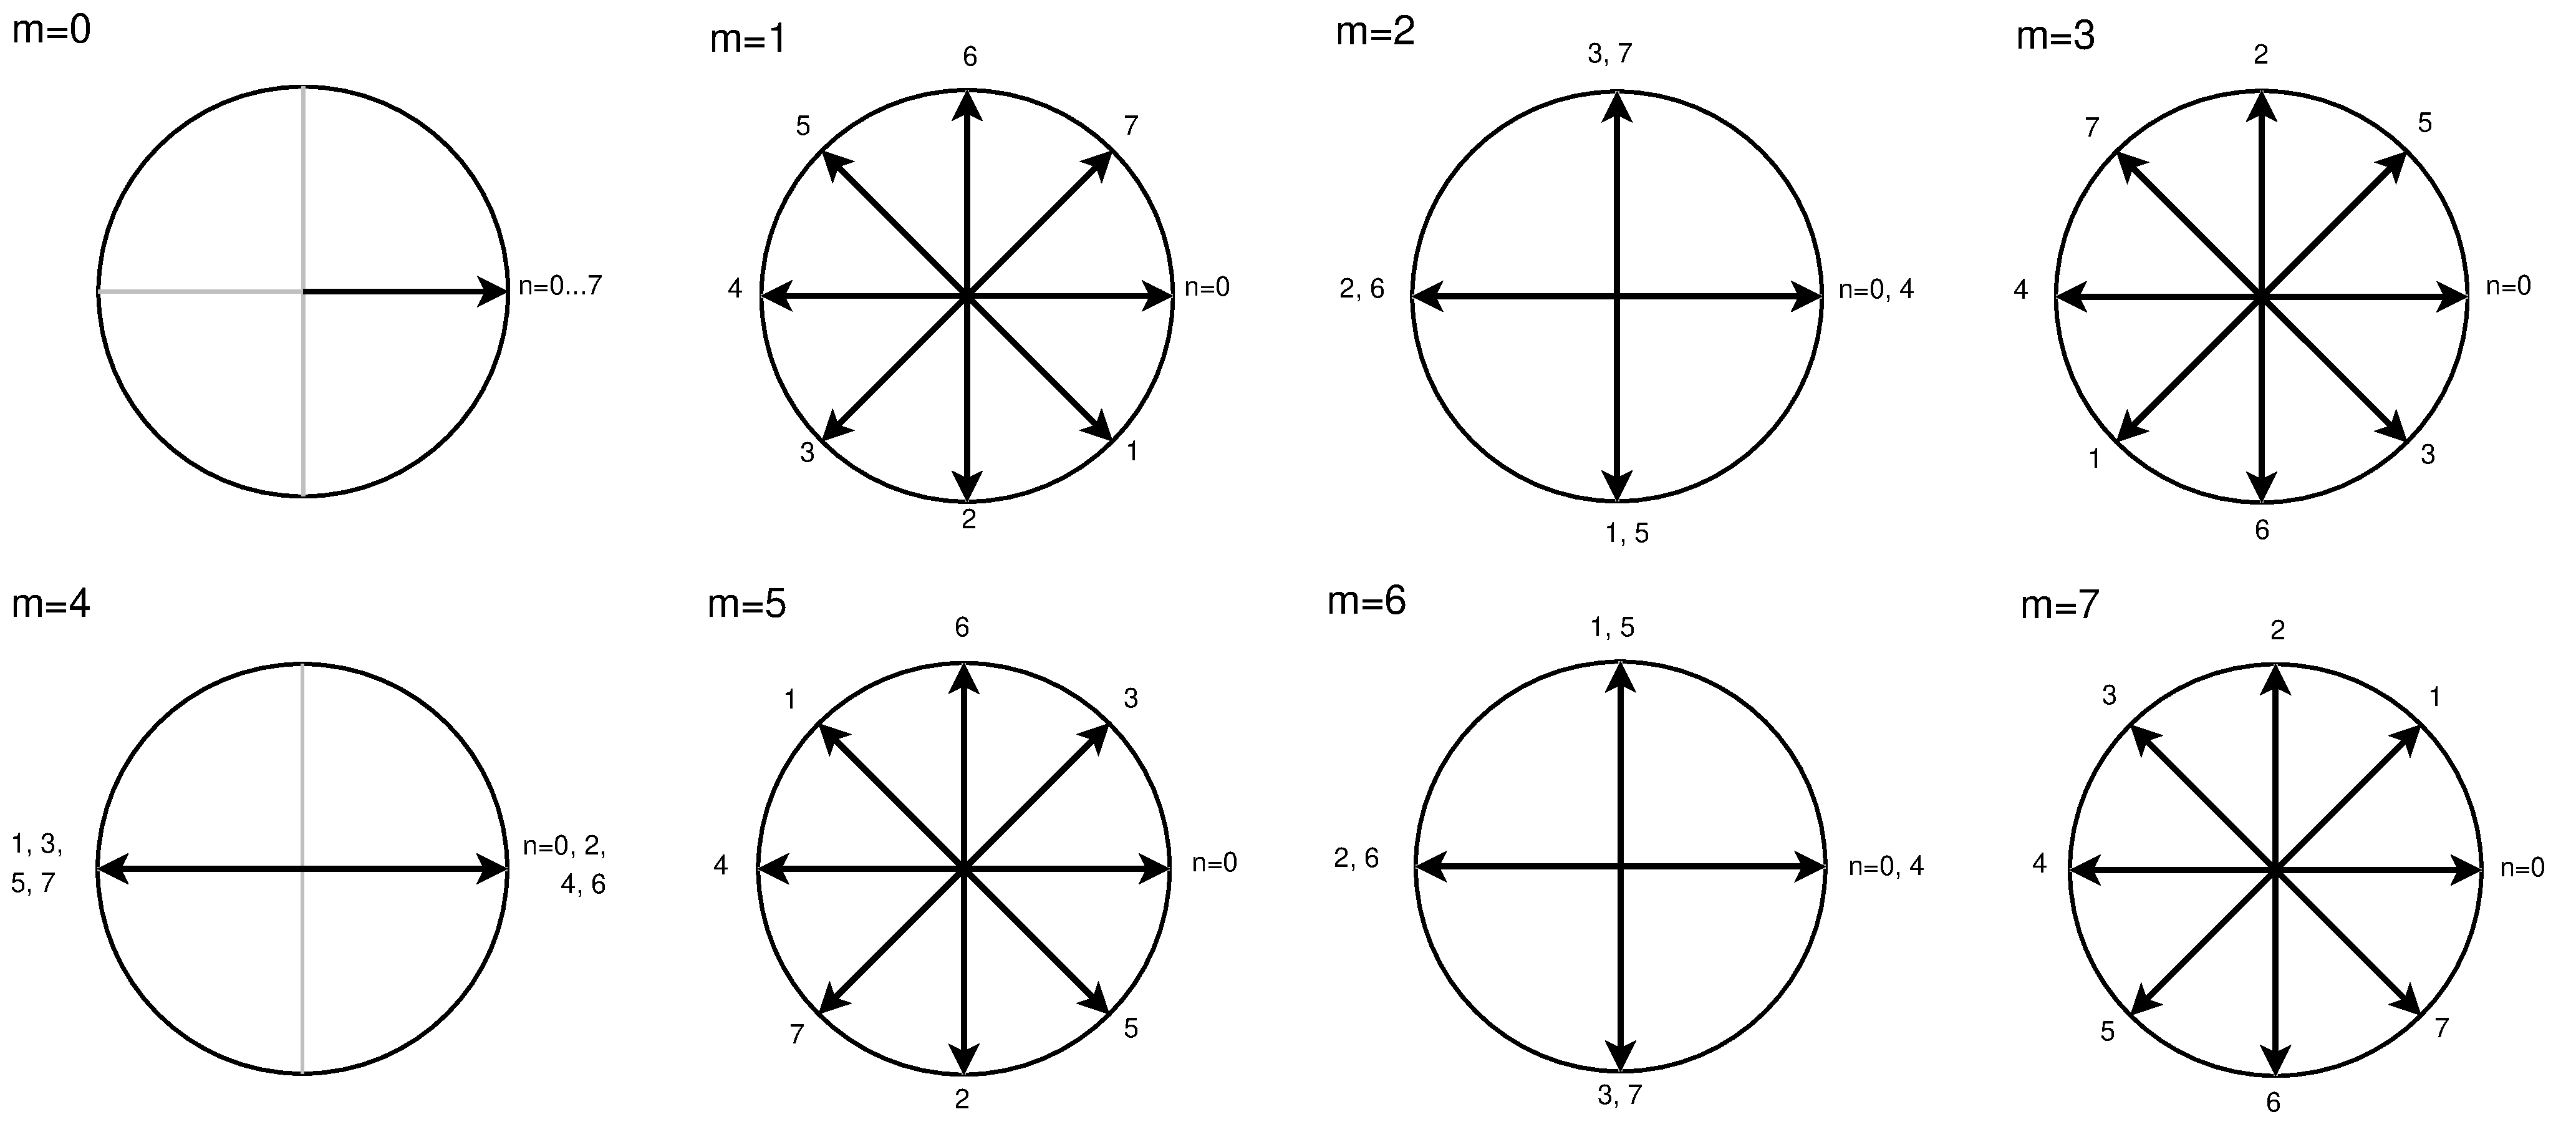
\includegraphics[width=1\textwidth]{img/Twiddlefaktoren_Einheitskreis.eps}
 \caption{Twiddlefaktoren der 8$\times$8-Matrix, aufgeteilt auf die Laufindizes $m$ und $n$. $m$ bezieht sich auf das Element im Ausgangsvektor $\vec{X}$, $n$ auf den Eingangsvektor $\vec{x}$. Siehe auch Gl. (\ref{eq:dft}) }
 \label{pic:Twiddlefaktoren_Darstellung8x8}
\end{figure}

\vspace{0.5cm}


 

\begin{minipage}{0.9\textwidth}
\begingroup
 \renewcommand*{\arraystretch}{0.95} % Zeilenabstand der Tabelle

\begin{center}
  \[
   \stackrel{\mbox{$Re\{W\}$}}{
    \begin{bmatrix}
     \myboxOnePos 	& \myboxOnePos 		& \myboxOnePos 	& \myboxOnePos 		& \myboxOnePos 	& \myboxOnePos 		& \myboxOnePos 	& \myboxOnePos \\
     \myboxOnePos 	& \myboxSqrtPos 	& \myboxZero 	& \myboxSqrtNeg		& \myboxOneNeg	& \myboxSqrtNeg		& \myboxZero	& \myboxSqrtPos \\
     \myboxOnePos 	& \myboxZero 		& \myboxOneNeg 	& \myboxZero 		& \myboxOnePos 	& \myboxZero 		& \myboxOneNeg 	& \myboxZero \\
     \myboxOnePos 	& \myboxSqrtNeg 	& \myboxZero 	& \myboxSqrtPos 	& \myboxOneNeg 	& \myboxSqrtPos 	& \myboxZero 	& \myboxSqrtNeg \\
     \myboxOnePos 	& \myboxOneNeg 		& \myboxOnePos 	& \myboxOneNeg 		& \myboxOnePos 	& \myboxOneNeg 		& \myboxOnePos 	& \myboxOneNeg \\
     \myboxOnePos 	& \myboxSqrtNeg 	& \myboxZero 	& \myboxSqrtPos 	& \myboxOneNeg 	& \myboxSqrtPos 	& \myboxZero 	& \myboxSqrtNeg \\
     \myboxOnePos 	& \myboxZero 		& \myboxOneNeg 	& \myboxZero 		& \myboxOnePos 	& \myboxZero 		& \myboxOneNeg 	& \myboxZero \\
     \myboxOnePos 	& \myboxSqrtPos 	& \myboxZero 	& \myboxSqrtNeg		& \myboxOneNeg	& \myboxSqrtNeg		& \myboxZero	& \myboxSqrtPos 
    \end{bmatrix}
   }
   \hspace{1cm}
   \stackrel{\mbox{$Im\{W\}$}}{
    \begin{bmatrix}
     \myboxZero 	& \myboxZero 		& \myboxZero 	& \myboxZero 		& \myboxZero 	& \myboxZero 		& \myboxZero 	& \myboxZero \\
     \myboxZero 	& \myboxSqrtNeg 	& \myboxOneNeg 	& \myboxSqrtNeg		& \myboxZero	& \myboxSqrtPos		& \myboxOnePos	& \myboxSqrtPos \\
     \myboxZero 	& \myboxOneNeg 		& \myboxZero 	& \myboxOnePos 		& \myboxZero 	& \myboxOneNeg 		& \myboxZero 	& \myboxOnePos \\
     \myboxZero 	& \myboxSqrtNeg 	& \myboxOnePos 	& \myboxSqrtNeg 	& \myboxZero 	& \myboxSqrtPos 	& \myboxOneNeg 	& \myboxSqrtPos \\
     \myboxZero 	& \myboxZero 		& \myboxZero 	& \myboxZero 		& \myboxZero 	& \myboxZero 		& \myboxZero 	& \myboxZero \\
     \myboxZero 	& \myboxSqrtPos 	& \myboxOneNeg 	& \myboxSqrtPos		& \myboxZero 	& \myboxSqrtNeg 	& \myboxOnePos 	& \myboxSqrtNeg \\
     \myboxZero 	& \myboxOnePos 		& \myboxZero 	& \myboxOneNeg 		& \myboxZero 	& \myboxOnePos 		& \myboxZero 	& \myboxOneNeg \\
     \myboxZero 	& \myboxSqrtPos 	& \myboxOnePos 	& \myboxSqrtPos		& \myboxZero	& \myboxSqrtNeg		& \myboxOneNeg	& \myboxSqrtNeg 
    \end{bmatrix}
   }
  \]
\vspace{0.5cm}
  Legende: $\myboxOnePos$ = 1 \quad $\myboxOneNeg$ = -1 \quad $\myboxZero$ = 0 \quad $\myboxSqrtPos$ = $\nicefrac{\sqrt{2}}{2}$ \quad $\myboxSqrtNeg$ = -$\nicefrac{\sqrt{2}}{2}$
  \captionof{figure}{Matrix-Darstellung der 8x8-DFT-Twiddlefaktoren aufgeteilt nach Real- und Imaginärteil}
  \label{pic:MatrizenDarstellungTwiddlefaktoren}
\end{center}
\endgroup
\end{minipage}


\vspace{0.5cm}


Sowohl der Abbildung \ref{pic:Twiddlefaktoren_Darstellung8x8} als auch insbesondere der Darstellung \ref{pic:MatrizenDarstellungTwiddlefaktoren} lassen sich sehr gut die 
Symmetrien erkennen, die diese Twiddlefaktormatrix so vorteilhaft machen.

 % \section{Überlegungen DCT vs. DFT}
 Die \gls{2d-dft} findet häufig in der Bildverarbeitung Anwendung und lässt sich gut auf unser Problem übertragen.
 
 \section{Abschätzung des Rechenaufwandes}\label{sec:abschaetzung_Rechenaufwand}
\subsection{Komplexe Multiplikation}

Im allgemeinen Fall müssen gemäß Gl. \ref{eq:komplexe_Multiplikation} bei der komplexen Multiplikation vier einfache Multiplikation sowie zwei Additionen durchgeführt werden.

\begin{align}\label{eq:komplexe_Multiplikation}
\begin{split}
 e + jf &= (a + jb) \cdot (c + jd)\\
        &= a \cdot c + j(a \cdot d) + j(b \cdot c) + j^2(b \cdot d)\\
        &= a \cdot c + b \cdot d + j(a \cdot d + b \cdot c)
\end{split}
\end{align}


Da das Signal $x_{sens}(t)$ der Sensoren rein reell ist, reduziert sich der Aufwand wie in Gl. \ref{eq:halb_komplexe_Multiplikation} zu sehen auf zwei Multiplikationen und eine Addition.

\begin{align}\label{eq:halb_komplexe_Multiplikation}
\begin{split}
 e + jf &= a \cdot (c + jd)\\
        &= a \cdot c + j(a \cdot d)\\
\end{split}
\end{align}

Wie bereits unter \ref{sec:AnalyseBewertungTwiddlefaktornMatrizen} auf Seite \pageref{sec:AnalyseBewertungTwiddlefaktornMatrizen} erörtert, kann sogar die komplexe 
Twiddlefaktor-Matrix in diesem speziellen Fall als rein reell betrachtet werden. Somit bleibt von der anfangs komplexen Multiplikation nur eine rein reelle Multiplikation und
in 50$\percent$ der Fälle die Bildung des 2er-Komplements übrig, was erheblich Rechenaufwand erspart.

\begin{equation}
 X_{Sens}(f) = W \cdot x_{Sens}(t) \quad \textnormal{: ``rein reell''}
\end{equation}
  

\subsection{Matrizenmultiplikation}
Die \gls{dft} kann als Summation oder als Matrixmultiplikation geschrieben werden, wobei sich letzteres auf einem \gls{asic} bedeutend besser implementieren lässt. 
Gleichung \ref{eq:dft_matrixmultiplication} stellt die \gls{dft} als Matrizenmultiplikation dar, wobei $x(t)$ der Eingangsvektor (bzw. -matrix) im Zeitbereich und $W$ 
die Twiddlefaktormatrix ist.

\begin{align}\label{eq:dft_matrixmultiplication}
 X(f) = F(k) = W \cdot x(t) = W \cdot f(m)
\end{align}


Betrachtet wird zunächst die Multiplikation eines Vektors mit einer Matrix. 

\begingroup
\renewcommand*{\arraystretch}{1.0}

 \[
  \stackrel{\mbox{$X(f) = \mathcal{F}\{x(t)\}$}}{
  \begin{bmatrix}%
   \myBlackBox \\
   \myLightgrayBox \\
   \myLightgrayBox \\
   \myLightgrayBox
  \end{bmatrix}
  }
  =
  \stackrel{\mbox{$W$}}{
   \begin{bmatrix}
    \myBlackBox 	& \myBlackBox 		& \myBlackBox 		& \myBlackBox \\
    \myLightgrayBox 	& \myLightgrayBox 	& \myLightgrayBox 	& \myLightgrayBox \\
    \myLightgrayBox 	& \myLightgrayBox 	& \myLightgrayBox 	& \myLightgrayBox \\
    \myLightgrayBox 	& \myLightgrayBox 	& \myLightgrayBox 	& \myLightgrayBox
   \end{bmatrix}
  }
  \cdot
  \stackrel{\mbox{$x(t)$}}{
   \begin{bmatrix}
    \myBlackBox \\
    \myBlackBox \\
    \myBlackBox \\
    \myBlackBox
   \end{bmatrix}
  }
 \]
\endgroup

 \vspace{1cm}  
  
 \[
  \stackrel{\mbox{$X(f) = \mathcal{F}\{x(t)\}$}}{
   \begin{bmatrix}
    \myBlackBox 	& \myBlackBox 		& \myBlackBox 		& \myBlackBox \\
    \myDarkgrayBox 	& \myDarkgrayBox 	& \myDarkgrayBox 	& \myDarkgrayBox \\
    \myGrayBox 		& \myGrayBox 		& \myGrayBox 		& \myGrayBox \\
    \myLightgrayBox 	& \myLightgrayBox 	& \myLightgrayBox 	& \myLightgrayBox 
   \end{bmatrix}
  }
  =
  \stackrel{\mbox{$W$}}{
   \begin{bmatrix}
    \myBlackBox 	& \myBlackBox 		& \myBlackBox 		& \myBlackBox \\
    \myDarkgrayBox 	& \myDarkgrayBox 	& \myDarkgrayBox 	& \myDarkgrayBox \\
    \myGrayBox 		& \myGrayBox 		& \myGrayBox 		& \myGrayBox \\
    \myLightgrayBox 	& \myLightgrayBox 	& \myLightgrayBox 	& \myLightgrayBox 
   \end{bmatrix}
  }
  \cdot
  \stackrel{\mbox{$x(t)$}}{
   \begin{bmatrix}
    \myBlackBox & \myBlackBox & \myBlackBox & \myBlackBox \\
    \myBlackBox & \myBlackBox & \myBlackBox & \myBlackBox \\
    \myBlackBox & \myBlackBox & \myBlackBox & \myBlackBox \\
    \myBlackBox & \myBlackBox & \myBlackBox & \myBlackBox 
   \end{bmatrix}
  }
 \]

 \[
  X(f)' = F(k,l) = W \cdot F(k) = W \cdot x(t) \cdot W
 \]
 
 \[
  \stackrel{\mbox{$X(f)' = \mathcal{F}\{X(f)\}'$}}{
   \begin{bmatrix}
    \myBlackBox 	& \myBlackBox 		& \myBlackBox 		& \myBlackBox \\
    \myDarkgrayBox 	& \myDarkgrayBox 	& \myDarkgrayBox 	& \myDarkgrayBox \\
    \myGrayBox 		& \myGrayBox 		& \myGrayBox 		& \myGrayBox \\
    \myLightgrayBox 	& \myLightgrayBox 	& \myLightgrayBox 	& \myLightgrayBox 
   \end{bmatrix}
  }
  =
  \stackrel{\mbox{$X(f)$}}{
   \begin{bmatrix}
    \myBlackBox 	& \myBlackBox 		& \myBlackBox 		& \myBlackBox \\
    \myDarkgrayBox 	& \myDarkgrayBox 	& \myDarkgrayBox 	& \myDarkgrayBox \\
    \myGrayBox 		& \myGrayBox 		& \myGrayBox 		& \myGrayBox \\
    \myLightgrayBox 	& \myLightgrayBox 	& \myLightgrayBox 	& \myLightgrayBox 
   \end{bmatrix}
  }
  \cdot
  \stackrel{\mbox{$W$}}{
   \begin{bmatrix}
    \myBlackBox & \myBlackBox & \myBlackBox & \myBlackBox \\
    \myBlackBox & \myBlackBox & \myBlackBox & \myBlackBox \\
    \myBlackBox & \myBlackBox & \myBlackBox & \myBlackBox \\
    \myBlackBox & \myBlackBox & \myBlackBox & \myBlackBox 
   \end{bmatrix}
  }
 \]
 

  \subsection{Gegenüberstellung Butterfly / Matrixmultiplipation} 
  Die \gls{dft} wurde als Matrixmultiplikation implementiert, nachfolgend soll dies begründet und ein Vergleich beider Varianten erfolgen.
  
  Zu einem frühen Zeitpunkt der Überlegungen 
  an dieser Arbeit gab es noch die Idee die \gls{dft} so flexibel wie möglich zu halten, um unkompliziert auf andere Größen wechseln zu können.
  Hierfür sollten alle Koeffizienten der Twiddlefaktormatrix ladbar sein sowie die Größe der Matrix über eine globale Deklaration variabel gehalten werden.
  Diese Herangehensweise bedingt die Implementation als Matrixmultiplikation. Die Hoffnung der Projektgruppe bestand darin, dass das Synthesewerkzeug den 
  VHDL-Code soweit optimiert, dass dies nicht händisch erfolgen müsste.
  Als klar war, dass sie Optimierung nicht so tief greift, wurden die entsprechenden Schritte manuell umgesetzt. 
  
  Die Implementierung des Butterfly-Algorithmus nach Cooley und Tukey stellt eine effiziente Berechnung der \gls{dft} dar. 
  
  
  \subsection{Gegenüberstellung reelle / komplexe Eingangswerte}
  Die Sensormatrix liefert für jeden Pixel einen Sinus- und Kosinuswert. Diese können für die Berechnung der DFT zu einer komplexen Zahl zusammengefasst werden. 
  Auf diese Weise lässt sich die Berechnung mathematisch kompakter schreiben. Dadurch, dass eine komplexe Multiplikation auf vier reellen Multiplikationen basiert,
  ist es jedoch möglich, dass die Anzahl reeller Multiplikationen hierdurch derer bei der getrennten Berechnung und anschließenden Zusammenführung übersteigt.
  
  Bei der Berechnung der DFT 
 
  
 \subsection{Anzahl der benötigten Multiplikationen}
 \subsection{Optimierte Matrixmultiplipation bezogen auf 8x8}

 
 
 
\chapter{Entwurf}

 

 
 
 
 
 \section{Entwicklungsstufen}
\subsection{Multiplikation}

Zeigen, welche Bits heraus genommen werden müssen! und belegen warum.

\subsection{Addierer}
CLA, RC, in einem Takt

\subsection{Konstantenmultiplikation}
Dieser Punkt muss irgendwie mit der Implementierung des Konstantenmultiplizierers zusammengeführt werden.

Der duale Wert lässt sich am einfachsten mit der Matlab-Funktion \texttt{fi()} ermitteln. Der Funktion werden hierfür Kommagetrennt der Deziamlwert, 1 für vorzeichenbehaftet,
die gesamte Anzahl an Stellen (13) und die Anzahl der Nachkommastellen (10) übergeben. Der vollständige Aufruf sieht dann wie folgt aus:

% \begin{lstlisting}[language=matlab, frame=false, numbers=none, keywordstyle=\color{black},rulecolor=\color{white}]
% val=fi(sqrt(2)/2,1,13,10)
% \end{lstlisting}
\texttt{val=fi(sqrt(2)/2,1,13,10)}

Der erzeugte Datentyp hat unter anderem die Eigenschaften \texttt{val.bin}, welche einem mit $0001011010100$ den Wert als Binärzahl zurück gibt, 
\texttt{val.double} gibt den approximierten Dezimalwert mit 0,70703125 zurück und \texttt{val.dec} interpretiert den Dualwert als Integer, was 724 entspricht.
Letzterer ist wichtig zu kennen, um die Werte der Simulation nachvollziehen zu können.

Der Berechnung aus Gleichung (\ref{eq:abweichungWurzel2halbe}) kann entnommen werden, dass die Abweichung weit unter einem Prozent liegt.

\begin{equation}\label{eq:abweichungWurzel2halbe}
 \frac{100}{\dfrac{\sqrt{2}}{2}}\cdot 0,70703125 = 99,989\%
\end{equation}



\subsection{1D-DFT mit Integer-Werten}
 
\subsection{2D-DFT mit Integer-Werten}

\subsection{2D-DFT mit Werten SQ-Format}

\subsection{Zusammenhang von DFT und IDFT bei der Matrixmultiplikation}

Durch die umgekehrte Drehrichtung des komplexen Zeigers in Gleichung (\ref{eq:idft}) werden in der Matrizenschreibweise die Zeilen 2 und 8, 3 und 7 sowie 4 und 6 vertauscht.
Nachvollziehen lässt sich das gut anhand der Grafik (\ref{pic:Einheitskreis_Faktoren}). 
Verdeutlicht wird das vorgehen in Abbildung \ref{pic:IDFT_Zeilentausch}.

\begin{figure}[ht]
 \centering
 \includegraphics[width=0.4\textwidth]{img/IDFT_Zeilentausch.png}
 \caption{Um von der DFT zur IDFT zu kommen, müssen bei der Matrixmultiplikation die Zeilen 2 und 8, 3 und 7 sowie 4 und 6 der Twiddlefaktormatrix vertauscht werden.}
 \label{pic:IDFT_Zeilentausch}
\end{figure}



\section{Test der Matrixmultiplikation}
Unter anderem weil NC\,Sim bzw. dessen Unterprogramm SimVision zur Anzeige von Signalverläufen (Waveform) nur Integer darstellen kann und bei als Vektor gebündelten Signalen 
diese nicht einmal als vorzeichenbehaftet (signed), wurde der Einfachheit halber zunächst die Berechnung als Ganzzahl-Multiplikation mit dem Faktor 3 betrachtet. 
Da es bei diesem Faktor und den gewählten Eingangswerten nicht zu einem 
Überlauf kommen kann, war es zu diesem Zeitpunkt noch nicht nötig, sich Gedanken über die Breite des Ergebnisvektors bzw. den Ausschnitt daraus für die weitere
Berechnung zu machen. Deshalb konnte an dieser Stelle noch auf den Bitshift zur Halbierung der Werte verzichtet werden.

Erst als der Faktor $\frac{\sqrt{2}}{2}$ übernommen wurde, wurden die Ergebnisse breiter als der Vektor für die weitere Berechnung an Bits zur Verfügung stellt.

${\frac{\sqrt{2}}{2}}_{10}$ = $0001011010100_2$ in S2Q10, als Integer betrachtet jedoch $724_{10}$.

Daraus folgt, dass ein Teil der Bits abgeschnitten werden müssen. Da die Dualzahlen jetzt im S1Q10-Format betrachtet werden, es sich also um Kommazahlen handelt,
müssen die hinteren Bits abgeschnitten werden. Zudem können vorne Bits ohne Informationsverlust gestrichen werden, da durch die Multiplikation ein weiteres 
Negations-Bit dazugekommen ist und auf Grund des gegebenen Faktors der Wertebereich vorne nie ganz ausgenutzt wird. (Verifizieren / Belegen!)


\section{Implementierung des Konstantenmultiplizieres}\label{sec:Konstantenmultiplizierer}

Anfangs wurde angenommen, dass Multiplikationen mit den Twiddlefaktoren $\pm 1$ und $\pm\frac{\sqrt{2}}{2}$ durchgeführt werden müssen. 
Dass bei einer optimierten 8x8-DFT wegen des explizieten ausprogrammierens der Berechnungen die Multiplikation mit $\pm1$ wegfällt, wurde recht schnell klar.
Erst bei genauer Betrachtung der Twiddlefaktor-Matrix viel auf, dass in jeder Zeile gleich viele Additionen wie Subtraktionen vorhanden sind. Durch Umsortieren 
ist es dadurch möglich auf das Invertieren der Eingangswerte sowie den hierfür benötigten Takt und die Inverter zu verzichten. Weiter wird auch nur die Multiplikation
mit $+\frac{\sqrt{2}}{2}$ benötigt.

\subsection{Syntheseergebnis eines 13 Bit Konstantenmultiplizierers}\label{sec:SyntheseergebnisKonstantenmultiplizierer}
\begin{figure}[!ht]
\centering  
 %\fbox{
  \includegraphics[width=1\textwidth]{img/13Bit_Konstantenmultiplizierer_Netlist.png}
  %}
  \caption{13 Bit Konstantenmultiplizierer für $\frac{\sqrt{2}}{2} = 0.70711 \simeq 0.70703125 = 0001011010100_2$ in Encounter; Eingang links, Ausgang rechts}
  \label{pic:Konstantenmultiplizierer}
\end{figure}



\begin{table}[!ht]
 \caption{Vergleich Konstanten- mit regulärem Multiplizierer}
 \label{tab:VergleichMultiplizierer}
 \begin{tabular}{ccc}
 \hline
				& Konstantenmultiplizierer 	& regulärer Multiplizierer\\
  \hline	
  Gatter			& 27				& 175 \\
  Fläche (Prozess: 350nm)	& $\SI{6612}{um^2}$		& $\SI{23261}{um^2}$\\
  \hline
 \end{tabular}
\end{table}





Der vollständige Gate-Report befindet sich in Abschnitt \ref{src:rc_gate_report} auf Seite \pageref{src:rc_gate_report}



\subsection{Syntheseergebnis für die Bildung des Zweierkomplements eines 13 Bit Vektors}\label{sec:SyntheseergebnisBildungZweierkomplement}

Zum Vergleich mit dem Konstantenmultiplizierers aus Abb. \ref{pic:Konstantenmultiplizierer} soll in Abb. \ref{pic:13BitInverter} die nicht expliziet implementierte aber in Abschnitt
\ref{sec:GegenüberstellungRelleKomplexeEingangswerte} erwähnte Negierung von Zahlen gezeigt werden.

\begin{figure}[htpb]
\centering
\includegraphics[width=0.99\textwidth]{img/13Bit_Inverter_Netlist.png}
\caption{Netzliste einer Einheit zur Bildung des 2er-Komplements eines 13 Bit Vektors; Eingang links, Ausgang rechts}
\label{pic:13BitInverter}
\end{figure}

Für die Negierung eines 13 Bit Vektors hat das Synthesewerkzeug \texttt{encounter} 22 Standardzellen verwendet. Das sind knapp doppelt so viele Gatter, wie der Vektor 
Bits breit ist. Der Unterschied zum Konstantenmultiplizierer fällt somit sehr gering aus. 
Wie zu sehen, handelt es sich fast ausschließlich um Inverter und Addierer. In Abschnitt \ref{sec:Integer2erKomplement} wurde bereits beschrieben, dass für die Bildung des
2er-Komplements zunächst alle Bits invertiert werden müssen. Abschließend wird auf den Vektor 1 LSB addiert. 
Beide Pfade weisen die gleiche Länge auf und verwenden überwiedend die selben
Gattertypen, weshalb darauf geschlossen werden kann, dass die maximale Gatterlaufzeit in der gleichen Größenordnung liegen muss.



\subsection{Gegenüberstellung der Konstantenmultiplikation und der Bildung des 2er-Komplements}

Unter diesem Punkt sollen die Konstantenmultiplikation und die Bildung des 2er-Komplements unter Aspekten der benötigten Zeit und des benötigten Platzes auf einem Chip 
betrachtet werden. Um einen Eindruck hiervon zu erhalten, werden im Kapitel Entwurf in den Abschnitten \ref{sec:SyntheseergebnisKonstantenmultiplizierer} und
\ref{sec:SyntheseergebnisBildungZweierkomplement} jeweils die Schaltnetzte 
%für die Negation mittels 2er-Komplement und die Multiplikation mit einem konstanten Faktor 
gezeigt.
Wie dort erläuter, lässt sich anhand dieser sagen, dass es bei dieser Art der Implementierung keinen zeitlichen Gewinn gibt, da beide kritischen Pfade etwa gleich lang 
sind. Für die knapp $\nicefrac{1}{4}$ mehr Gatter bei der Multiplikation ist auch ein größerer Vertrahtungsaufwandt erforderlich, sodass die Konstantenmultiplizierer
auf einem Chip eine etwas größere Fläche beanspruchen. Da es sich hier insgesamt aber um sehr wenige Gatter handelt, wirkt sich dies erst bei sehr vielen Instanzen aus.
Es kann an dieser Stelle deshalb festgehalten werden, dass dieser Unterschied nicht als entscheidend geltend gemacht werden kann.
 
 
 
 
 \section{Kompromiss aus benötigter Chipfläche und Genauigkeit des Ergebnisses}
Dieser Abschnitt passt hier nicht so richtig hin! Aber wo sonst?

Durch die Begrenzung der Bitbreite ist es nötig nach jeder Addition den Wert zu halbieren. Hierbei steigt die Abweichung gegenüber einer verlustfreien Berechnung immer dann, 
wenn das letzte eine 1 ist. Im Mittel ist dies bei der Hälfte der Additionen der Fall. In 50$\%$ aller Fälle wird also der Wert um ein halbes LSB zu viel verringert.
Bei der Multiplikation verdoppelt sich sogar die resultierende Bitbreite. Da mit dem vollständigen 13 Bit Vektor nach der Addition weitergerechnet wird, muss die Konstante
ebenfalls in 13 Bit hinterlegt sein. Deshalb hat das Ergebnis 26 Bit, von denen für die weitere Berechnung wieder nur 12 übernommen werden. In den Abbildungen 
\ref{pic:AkkumulationUngeradeSpalten} und \ref{pic:AkkumulationGeradeSpalten} wird das hier beschriebene Vorgehen veranschaulicht. Bei diesem Verfahren
kommt es unweigerlich zur Akkumulation von Fehlern.
 
Da für die Berechnung einer Zahl der 1D-DFT je nach Zeile entweder 8 oder 12 Werte akkumuliert sowie 0 bis 4 Werte multipliziert werden und für die 2D-DFT entsprechend doppelt 
so viele, akkumulieren sich zwangsläufig Fehler. Bei 12 Bit Eingangswerten wäre ein 47? Bit Ausgangsvektor nötig, um dies vollständig zu vermeiden. Dies ist jedoch aus u.a.
Platzgründen nicht umsetzbar.

Mit jeder Addition kommt 1\,Bit dazu. So werden aus 12\,Bit bis zur Multiplikation 15 (12 + $\log_2(8)$), 8 = Anzahl der Zahlen die mit $\tfrac{\sqrt{2}}{2}$ multipliziert
werden müssen. Bei der Multiplikation verdopplet sich der Wert, also 30 und eine letzte Addition macht 31.
Beim zweiten Durchlauf werden es so (31+3)$\cdot$2+1=69\,Bit.

$\Rightarrow$ Anhand eines Simulationsbeispiels zeigen, dass die mit VHDL berechneten Werte immer kleiner als die in Matlab berechneten sind.


\section{Entwickeln der 2D-DFT in VHDL}

Ziel ist es die gleiche DFT-Einheit für beide DFTs zu verwenden

Zähler für 64 Werte kann als 6 Bit Vektor realisiert werden, der bei 63 einen Überlauf hat und wieder bei 0 anfängt.

Vorderen 3 Bit sind die der Zeile, die hinteren für die Spalte.

Das dritte Bit von vorne sagt einem, ob es eine gerade oder ungerade Zeile ist.


 
 
 
Die in Gleichung (\ref{eq:2D-DFT_MatrixMult}) beschriebene Berechnung der 2D-DFT lässt sich auch wie folgt schreiben:

\begin{align}
 X &= W \cdot x \cdot W \nonumber \\
   &= \left(x^T\cdot W\right)^T\cdot W \label{eq:MatMultTranspose1} \\
   &= X^* \cdot W \nonumber\\
   &= \left(\left(x\cdot W\right)^T\cdot W\right)^T \label{eq:MatMultTranspose2}\\
   &= \left(X^{*T} \cdot W\right)^T \nonumber
\end{align}

In Matlab muss hierfür entweder die Funktion \texttt{transpose()} oder \texttt{.'} verwendet werden. Letzteres muss elementweise angewandt werden, da das Apostroph
alleine die komplex konjugiert Transponierte bildet.

Die alternativen Schreibweisen der 2D-DFT haben den Vorteil, dass in beiden Fällen die Eingangsmatrix auf der linken Seite steht. Möglich ist dies, da die 
Twiddlefaktormatrix identisch mit ihrer Transponierten ist.
Dass nun in den Gleichungen (\ref{eq:MatMultTranspose1}) und (\ref{eq:MatMultTranspose2}) sowohl die Eingangs- als auch die 1D-DFT-Matrix links steht, ist eine wichtige 
Voraussetzung dafür, dass mit der selben Recheneinheit mit der die 1D-DFT berechnet wird auch die 2D-DFT berechnet werden kann.
Die zweite Voraussetzung ist das Transponieren einer Matrix. Diese lässt sich durch spaltenweises Abspeichern und zeilenweises Auslesen der Ergebnis-Matrix realisieren.
Hierfür ist es lediglich notwendig die beiden Indizes, welche ein Matrixelement ansprechen, beim Speichern getauscht werden. Nun sind nun alle Voraussetzungen erfüllt, 
um beide Berechnungen mit der selben Einheit durch zu führen. In Grafik (\ref{pic:MatMultTranspose}) ist das hier beschriebene veranschaulicht.

(Auf diese Weise wird die direkte Weiterverarbeitung von Werten denkbar.)
 
\begin{figure}[htbp]
 \centering
 \includegraphics[width=0.95\textwidth]{img/MatMultTranspose2.png}
 \caption{Darstellung der Berechnung der 2D-DFT aus Gleichung (\ref{eq:MatMultTranspose2})}
 \label{pic:MatMultTranspose}
\end{figure}
 

\section{Direkte Weiterverarbeitung der Zwischenergebnisse}
Um die Anzahl an Gattern und somit den Flächenbedarf zu reduzieren ist es das Ziel, die Ergebnisse der \gls{1d-dft} aus der 1. Berechnungsstufe im nächsten Schritt direkt als 
Eingangswerte für die \gls{2d-dft} zu verwenden. Auf diese Weise würden 64$\cdot$2$\cdot$12 Bit = 1536 Bit = 1,5kBit = 192 Byte an Speicher eingespart werden.
Wie sich im Laufe der Entwicklung gezeigt hat, lässt sich das nicht nutzen. Das liegt daran, dass dazu übergegangen wurde, immer nur ein Element zur Zeit berechnet wird und die 
bereits errechneten demnach zwischengespeichert werden müssen. Dieser Ansatz wurde verfolgt, da der Entwicklungsaufwand in VHDL für die spaltenweise Berechnung der Ausgangswerte 
einfacher umzusetzen war und es zunächst nur um die mathematische Umsetzung und nicht um die Platzeffizienz auf einem Chip ging.

Unklar war zu diesem Zeitpunkt noch, wie der Speicher realisiert werden soll. In der finalen Variante des Chips soll es einen \gls{ram} geben, der als zentraler
Speicher von allen Komponenten genutzt wird. Da die Entwicklung im Projekt noch nicht soweit fortgeschritten ist und dies nicht zu den Aufgaben der vorliegenden Arbeit gehört,
wurde auf das Speichern in lokalen Speicherzellen ausgewichen, welche als Variable oder Signal im VHDL-Code definiert und von der Software als Flip-Flop synthetisiert werden.



%\section{Umsetzung der Optimierungen}
\section{Optimierte 8x8 DFT als Matrixmultiplikation}\label{sec:OptimierteMatrixmultiplikation}
Anfangs wurde in Betracht gezogen das 1er-Komplement zu verwenden, da hierbei zwei betragsmäßig identische Zahen sich nur durch ihr höchstwertigstes 
 Bit unterscheiden. Auf diese Weise könnte das selbe Resultat für den Imaginär- wie für den Realteil verwendet werden, das Vorzeichen würde sich über eine 
 einfache XOR-Verknüpfung beider MSB der Multiplikanden ergeben.
 Diesem Vorteil steht jedoch eine aufwändigere Subtraktion (bzw. Addition negativer Zahlen) gegenüber. Der zusätzliche Aufwand entspricht 
 etwa dem der Bildung des 2er-Komplements. Aus diesem Grund und da das 2er-Komplement deutlich verbreiteter ist sowie weitere Vorteile bringt wie 
 beispielsweise keine Doppeldeutigkeit durch eine negative Null hat, wurde sich hierfür entschieden.
 
 
 In späteren Analysen konnte festgestellt werden, dass sowohl für den Real- als auch den Imaginärteil gleichviele Multiplikationen mit positiven wie mit negativen Faktoren 
 durchgefürht werden müssen. Dies lässt sich anhand des Einheitskreises in Abb. \ref{pic:Einheitskreis_Faktoren} und der Abbildung \ref{pic:Twiddlefaktoren_Darstellung8x8}
 nachvollziehen. Aus Abschnitt \ref{sec:Matrixmultiplikation} ist bekannt, dass bei einer Matrixmultiplikation Elemente multipliziert und anschließend die Ergebnisse 
 aufsummiert. Da es das Kommutativgesetz erlaubt die berechneten Ergebnisse auch in einer anderen Reihenfolge zu addieren, 

 
   
 In Abbildung \ref{pic:MatrizenDarstellungTwiddlefaktoren} ist zu sehen, dass die 2., 4., 6., und 8. Zeile je vier nicht triviale und komplexe Faktoren enthält. 
 Darüber hinaus ist ersichtlich, dass für komplexe Eingangswerte in den genannten Zeilen 12 und in den übrigen 8 Multiplikationen erfolgen müssen. Dies kann anhand der 
 Gleichungen (\ref{eq:komplexe_Multiplikation}) und (\ref{eq:halb_komplexe_Multiplikation}) nachvollzogen werden.
 Das lässt sich ausnutzen, um keine Negationen der Eingangs- und Zwischenwerte durchführen zu müssen. 
 

 
 Darüber hinaus
 minimiert sich bei geschickter Anordnung das Risiko eines Überlaufs. Wie in Abschnitt \ref{sec:NumerischeUngenauigkeiten} erwähnt, ist dies nicht Gegenstand dieser Arbeit,
 weshalb der Einfachheit wegen zur Sicherheit dennoch nach jeder Addition oder Subtraktion das Ergebnis durch einen Bitshift halbiert wird. 
 Es sei an dieser Stelle lediglich angemerkt, dass über die Eingangswerte die Annahme getroffen werden kann, dass aufeinanderfolgende Werte das selbe Vorzeichen haben. 
 Dies ließe sich ausnutzen, um noch weiter die Wahrscheinlichkeit zu reduzieren, dass es zu einem Überlauf kommt. 
 

 




% Später wohl besser ins Kapitel Entwicklung
Dies hat zur Folge, dass ein sehr großer Wert entstehen kann, welcher Maßgebend für die Anzahl der Vorkommabits sein kann.
%
Wegen der Null im Imaginärteil der ersten Zeile der Twiddlefaktormatrix sind auch alle Imaginärteile der ersten Spalte der Ausgangsmatrix Null.
Bezogen auf den Imaginärteil gilt das Gleiche auch für die fünfte Zeile der Twiddlefaktormatrix. 
%
Da sich beim Realteil der fünften Zeile der Twiddlefaktormatrix der fünften Zeile positive und negative Einsen abwechseln, sind hier auch keinerlei Multiplikationen nötig.

Aus der anfänglichen Implementation bei der alle nicht trivialen Werte einer Berechnung die entweder mit $+\frac{\sqrt{2}}{2}$ oder $-\frac{\sqrt{2}}{2}$ multipliziert wurden,
einzelnd berechnet werden, wird mittels des Distributivgesetzes der gemeinsame Faktor ausgeklammert, sodass nur noch jeweils eine Multiplikation erforderlich ist.


Bei den weiteren Zeilen sind hingegen die Zahlen zur Hälfte positiv und zur anderen negativ. Außerdem enthalten die geraden Zeilen den Faktor $\pm\frac{\sqrt{2}}{2}$. 
Dies lässt sich ausnutzen, um die Anzahl der der Multiplikationen zu reduzieren. Zunächst können die 

Für jede gerade Zeile der DFT ist jeweils für den Real- und den Imaginärteil eine Multiplikation nötig, so dass sich insgesamt acht Multiplikationen ergeben
 
\subsection{W = transpose(W)}
 
 
\section{Berechnungsschema der geraden und ungeraden Zeilen}\label{sec:Berechnungsschema}

In Abbildung \ref{pic:AkkumulationUngeradeSpalten} ist die Berechnung der ungeraden Zeilen am Beispiel der ersten zu sehen.

\begin{figure}[htbp]
\centering
$a_{0} + a_{1} + a_{2} + a_{3} + a_{4} + a_{5} + a_{6} + a_{7}$\\

\vspace{0.5cm}
\begin{tabular}{ccccccccc}
Takt&\multicolumn{6}{l}{ } & & Bit\\
1&$\underbrace{a_{k0} + a_{k1}}$ &  &$ \underbrace{a_{k2} + a_{k3}}$ &  &$\underbrace{a_{k4} + a_{k5}}$ &  &$\underbrace{a_{k6} + a_{k7}}$ & 12\\
&\multicolumn{7}{l}{$\hspace{0.65cm} \Downarrow \hspace{2.3cm} \Downarrow \hspace{2.3cm} \Downarrow \hspace{2.3cm}\Downarrow$}&13\\
2&\multicolumn{3}{c}{$\underbrace{sum\_1\_1 \quad + \quad sum\_1\_2}$} & & \multicolumn{3}{c}{$\underbrace{sum\_1\_3 \quad + \quad sum\_1\_4}$} & 12\\
&\multicolumn{3}{c}{$\Downarrow$} & & \multicolumn{3}{c}{$\Downarrow$}&13\\
3&\multicolumn{7}{c}{$\underbrace{sum\_2\_1 \quad  \quad \quad \quad + \quad \quad \quad  \quad sum\_2\_2}$} & 12\\
&\multicolumn{7}{c}{$\Downarrow$}&13\\
&\multicolumn{7}{c}{$sum\_3\_1$} & 12\\
&\end{tabular}
%\captionof{figure}{Vorgehensweise der Akkumulation der ungeraden Spalten der Eingangswerte}
\caption{Vorgehensweise der Akkumulation der ungeraden Spalten der Eingangswerte.}
\label{pic:AkkumulationUngeradeSpalten}
\end{figure}
%\end{center}

\vspace{0.5cm}

Wie der linken Spalte zu entnehmen ist, werden 3 Takte für die Berechnungen der Werte aus den ungeraden Spalten der Eingangsmatrix bzw. ungeraden Zeilen der 1D-DFT-Matrix benötigt.
1. Takt für Additionen bzw. Subtraktionen und 2. sowie 3. Takt für das Aufsummieren. Der Bitvektor des Ergebnisses ist zwar 12 Bit breit, aber beim letzten Bitshift von 13 auf 12
werden nur 11 Bit übernommen. Es wird alo ein doppelter Bitshift vollzogen. Dies erfolgt, damit sowohl in den geraden als auch den ungeraden Zeilen gleich viele Bitshifts erfolgen
und die Werte somit identisch skaliert sind.

Die Berechnung der geraden Zeilen wird in Abbildung \ref{pic:AkkumulationGeradeSpalten} am Beispiel der zweiten Zeile gezeigt
\begin{figure}[htbp]
 \centering
 $a_0 - x_1 + x_0 - b_2 + x_2 - x_3 + a_4 - x_5 + x_4 - b_6 + x_6 - x_7$\\

 \vspace{0.3cm}
 
\begin{tabular}{ccccccccccccc}
Takt&\multicolumn{11}{c}{}&Bit\\
1 &$\underbrace{a_0 - x_1}$ &        &$ \underbrace{x_0 - b_2}$ &  &$\underbrace{x_2 - x_3}$ &  &$\underbrace{a_4 - x_5}$ &  &$\underbrace{x_4 - b_6}$ &$\underbrace{x_6 - x_7}$& &12\\
  &\multicolumn{11}{l}{$\hspace{0.5cm} \Downarrow \hspace{1.75cm} \Downarrow \hspace{2.4cm} \Downarrow \hspace{1.8cm}\Downarrow \hspace{1.8cm}\Downarrow \hspace{1.4cm}\Downarrow$}&13\\
2 &\multicolumn{3}{c}{$\underbrace{sum1\_1 \: + \: sum1\_2}$} & & \multicolumn{3}{c}{$\underbrace{sum1\_3 \: + \: sum1\_4}$} &\multicolumn{3}{c}{$\: \underbrace{sum1\_5 \: + \: sum1\_6}$}& &12\\
  &\multicolumn{3}{c}{$\Downarrow$}  & & \multicolumn{3}{c}{$\Downarrow$} & & \multicolumn{2}{c}{$\Downarrow$}& &13\\
3 &\multicolumn{7}{c}{$\underbrace{sum2\_1 \quad  \quad \quad \quad + \quad \quad \quad  \quad sum2\_2}$} & & & & &12\\
  &\multicolumn{7}{c}{$\Downarrow$}& & \multicolumn{2}{c}{$\Downarrow$}& &13\\
  &\multicolumn{7}{c}{$sum3\_1$}& & & & &13\\
  & & & & $\Downarrow$& & & & & \multicolumn{2}{c}{$\Downarrow$} & & 13\\
4 & & & & $\frac{\sqrt{2}}{2}$&\multicolumn{5}{c}{}& & &13\\
  & & & & $\Downarrow$& & & & & \multicolumn{2}{c}{$\Downarrow$ }& & 26\\
5 & & & \multicolumn{9}{c}{$\underbrace{sum4\_1 \:  \quad \quad \quad \quad \quad \quad + \quad \quad \quad \quad \quad \quad   sum2\_3}$} &12\\
  & & & \multicolumn{9}{c}{$\Downarrow$}&13\\
  & & & \multicolumn{9}{c}{$sum5\_1$}&12\\
\end{tabular}
\caption{Vorgehensweise der Akkumulation der geraden Spalten der Eingangswerte.}
\label{pic:AkkumulationGeradeSpalten}
\end{figure}

\vspace{1cm}
Auch hier ist der linken Spalte die Anzahl der benötigten Takte zu entnehmen. In diesem Fall werden 5 Takte für die Berechnungen benötigt. Diese setzen sich zusammen aus
1 Takt für Additionen bzw. Subtraktionen, 2.-3. sowie 5. Takt für das Aufsummieren und der 4. Takt für die Multiplikationen.

Wie rechts am Rand zu sehen, ergibt sich durch die Addition eine Bitbreitenerweiterung um 1 bzw. bei der Multiplikation eine Verdoppelung. Bei einer früheren 
Implementierung, die nur die 1D-DFT beherrschte, wurde zumindest die Erweiterung bei der Addition umgesetzt. Da bei der 2D-DFT die selbe Recheneinheit genutzt 
werden soll, wurde in Absprache mit dem ISAR-Team entschieden, dass die Summanden vor jeder Summation durch einen Bitshift nach rechts halbiert werden. Auf diese
Weise hat ein Additionsergebnis immer 13 Bit Breite. Durch den Bitshift kann das Resultat der 1D-DFT direkt als Eingang für die 2D-DFT verwendet werden. 

Zu bedenken gilt es bei einem Bitshift, dass das Ergebnis mit jedem Mal eine Division durch 2 erfährt. Bei hintereinander erfolgenden Bitshifts wird demnach durch $2^{N_B}$ geteilt, 
wobei $N_B$ die Anzahl der Bitshifts ist. Den beiden obigen Darstellungen der Summationen kann entnommen werden, dass, um ein Überlaufen des Bitvektors zu vermeiden es nötig ist,
drei respektive vier Bitshifts durch zu führen. Wie bereits erläutert erfolgt bei den ungeraden Zeilen abschließend ein doppelter Bitshift. Auf diese Weise ergibt sich für die
1D-DFT, dass das Ergebnis um den Faktor 16 kleiner ist, als beispielsweise bei der Berechnung mit Matlab. Da bei bei dem zweiten Durchlauf, um die 2D-DFT zu berechnen, ebenfalls 
durch 16 geteilt wird, ergibt sich insgesamt eine Division durch $2^{2\cdot4} = $ 256.

\subsection{Erwartete Anzahl benötigter Takte}
Aus den Abbildungen \ref{pic:AkkumulationUngeradeSpalten} und \ref{pic:AkkumulationGeradeSpalten} können die Takte die zur Berechnung der 1D- bzw. 2D-DFT benötigt werden 
abgeleitet werden.

Für ungeraden Zeilen sind je Element 3 Takte nötig und mit 8 Elementen pro Zeile und 4 ungeraden Zeilen errechnen sich so 3$\cdot$8$\cdot$4=96 Takte.
Analog errechnet sich für die ungeraden Zeilen mit je 5 Takten pro Element 5$\cdot$8$\cdot$4=160 Takte.
In der Summe ergeben sich so 96+160=256 Takte für die 1D-DFT. Da die 2D-DFT ohne Takte fürs Umspeichern oder ähnliches sofort im Anschluss berechnet werden kann, 
verdoppelt sich die Anzahl der Takte auf 512 für die vollständige Berechnung.



\section{Kompromiss aus benötigter Chipfläche und Genauigkeit des Ergebnisses}
Dieser Abschnitt passt hier nicht so richtig hin! Aber wo sonst?

Durch die Begrenzung der Bitbreite ist es nötig nach jeder Addition den Wert zu halbieren. Hierbei steigt die Abweichung gegenüber einer verlustfreien Berechnung immer dann, 
wenn das letzte eine 1 ist. Im Mittel ist dies bei der Hälfte der Additionen der Fall. In 50$\%$ aller Fälle wird also der Wert um ein halbes LSB zu viel verringert.
Bei der Multiplikation verdoppelt sich sogar die resultierende Bitbreite. Da mit dem vollständigen 13 Bit Vektor nach der Addition weitergerechnet wird, muss die Konstante
ebenfalls in 13 Bit hinterlegt sein. Deshalb hat das Ergebnis 26 Bit, von denen für die weitere Berechnung wieder nur 12 übernommen werden. In den Abbildungen 
\ref{pic:AkkumulationUngeradeSpalten} und \ref{pic:AkkumulationGeradeSpalten} wird das hier beschriebene Vorgehen veranschaulicht. Bei diesem Verfahren
kommt es unweigerlich zur Akkumulation von Fehlern.
 
Da für die Berechnung einer Zahl der 1D-DFT je nach Zeile entweder 8 oder 12 Werte akkumuliert sowie 0 bis 4 Werte multipliziert werden und für die 2D-DFT entsprechend doppelt 
so viele, akkumulieren sich zwangsläufig Fehler. Bei 12 Bit Eingangswerten wäre ein 47? Bit Ausgangsvektor nötig, um dies vollständig zu vermeiden. Dies ist jedoch aus u.a.
Platzgründen nicht umsetzbar.

Mit jeder Addition kommt 1\,Bit dazu. So werden aus 12\,Bit bis zur Multiplikation 15 (12 + $\log_2(8)$), 8 = Anzahl der Zahlen die mit $\tfrac{\sqrt{2}}{2}$ multipliziert
werden müssen. Bei der Multiplikation verdopplet sich der Wert, also 30 und eine letzte Addition macht 31.
Beim zweiten Durchlauf werden es so (31+3)$\cdot$2+1=69\,Bit.

$\Rightarrow$ Anhand eines Simulationsbeispiels zeigen, dass die mit VHDL berechneten Werte immer kleiner als die in Matlab berechneten sind.


 
 
%\section{Struktogramm}

%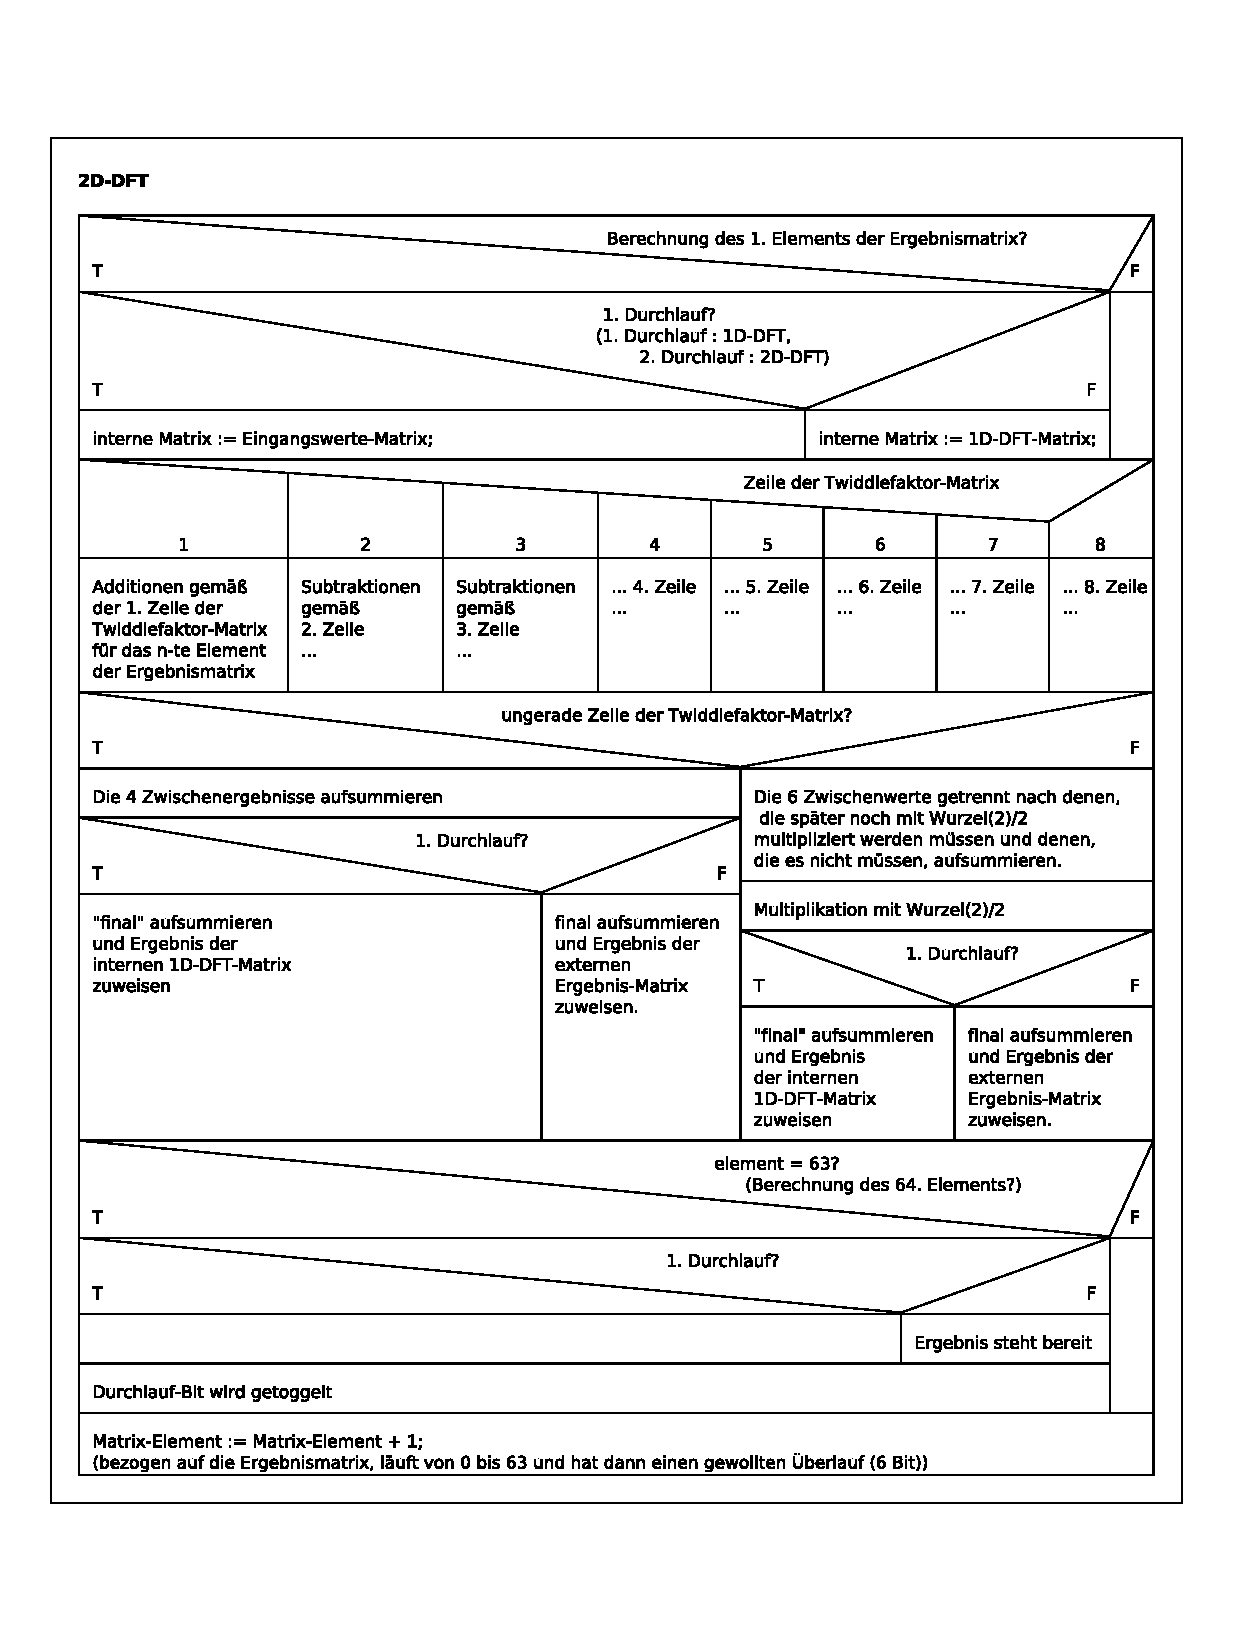
\includepdf{content/Struktogramm.pdf}

\section{Schema der Zustandsfolge}
test test

 \begin{figure}[t!]
 \centering
\begin{tikzpicture}[->,>=stealth',shorten >=1pt,auto,node distance=4.5cm,
                    semithick,initial text=nReset, initial where=above]
  \tikzstyle{every state}=[fill=white, text=black]
  %\tikzstyle{every initial where}=[above]
  

  \node[initial,state, circle split,minimum size=70pt] (A)                   {Idle};
  \node[state, circle split, minimum size=65pt]         (B) [below right of=A]{Twiddle\_Calc};
  \node[state, circle split, minimum size=65pt]         (C) [below right of=B]      {Additions\_1};
  \node[state, circle split, minimum size=65pt]         (D) [below of=C] {Additions\_2};
  \node[state, circle split, minimum size=65pt]         (E) [below left of=D] {Const\_mult};
  \node[state, circle split, minimum size=65pt]         (F) [above left of=E]      {Additions\_3};
  \node[state, circle split, minimum size=65pt]         (G) [above of=F]      {set\_ready\_bit};

  
   \path (A) edge (B) 
         (A) [loop left] edge(A)
         (B) [bend left=10] edge (C)
         (C) edge (D)
         (D) edge (B)
         (D) edge (E)
         (E) edge (F)
         (F) [bend right=10] edge (B)
         (F) [bend left=10] edge (G)
         (G) edge (B);
\end{tikzpicture}
\caption{Automatengraf}
\label{pic:Automatengraf}
\end{figure}


\section{UML-Diagramm}

% Define block styles
\tikzstyle{decision} = [diamond,                    draw, fill=blue!20, text width=6em, text badly centered, node distance=4cm, inner sep=0pt]
\tikzstyle{block} =    [rectangle, rounded corners, draw, fill=blue!20, text width=5em, text centered,       node distance=4cm, minimum height=5em, minimum width=7em]
\tikzstyle{smallblock} =    [rectangle, rounded corners, draw, fill=blue!20, text width=5em, text centered,       node distance=4cm, minimum height=2em, minimum width=3.5em]
\tikzstyle{wideblock} =    [rectangle, rounded corners, draw, fill=blue!20, text width=7em, text centered,       node distance=4cm, minimum height=5em, minimum width=7em]
\tikzstyle{verywideblock} =    [rectangle, rounded corners, draw, fill=blue!20, text width=15em, text centered,       node distance=4cm, minimum height=4em, minimum width=15em]
\tikzstyle{textblock} =    [rectangle, rounded corners, draw, fill=blue!20, text width=12em, text centered,       node distance=4cm, minimum height=4em, minimum width=10em]
\tikzstyle{dot}=[draw,shape=circle]

\tikzstyle{arrowline} = [draw, -latex']


    
\begin{tikzpicture}[auto, node distance = 1cm and 1cm, initial text=POR, initial where=above]
    % Place nodes
    \node [initial, smallblock] (start) {Idle};
    \node [decision, below of=start, node distance=3cm] (init) {IDFT?};
    \node [block, below right of=init, node distance=3cm] (Zeilenindex) {Zeilenindex tauschen};
    \coordinate[below of=init, node distance=3.5cm](Punkt_0);
    \node [decision, below of=Punkt_0, node distance=2cm] (Element_1) {Berechnung 1. Element?};
    \coordinate [right of=Element_1, node distance=4cm](c1);
    \node [decision, below of=c1, node distance=2cm] (Berechnung_1D_1) {Berechnung 1D-DFT?};
    
    \node [block, below of=Berechnung_1D_1, node distance=3cm] (überschreiben_mit_eingangswerten) {Zwischen- werte := 1D-DFT-Werten};
    \node [block, right of=überschreiben_mit_eingangswerten, node distance=4cm] (überschreiben_mit_1D_Werten) {Zwischen- werte := Eingangswerte};
    \node [block, left of=überschreiben_mit_eingangswerten, node distance=4cm] (Werte_beibehalten) {Zwischen- werte := Zwischen- werte};
    
    \node [dot, fill, inner sep=1pt, below of=überschreiben_mit_eingangswerten,node distance=1.5cm] (Punkt_1){};
    \node [decision,                 below of=Punkt_1,node distance=2cm] (Zustandsabfrage) {Zeilen- abfrage};
    
    \node [dot, fill, inner sep=1pt, below of=Zustandsabfrage,node distance=2cm] (Punkt_2){};
    \coordinate[below of=Punkt_2, node distance=0.5cm](Punkt_3);
    
    \node [textblock, right of=Punkt_2, node distance=3cm] (Zeile_1){Berechnungen entsprechend Zeile 1 der Twiddlefaktor-Matrix};
      
    \coordinate[below of=Punkt_3](Punkt_4);
    \coordinate[below of=Punkt_4,node distance=0.5cm] (Punkt_5);
    \node [textblock, right of=Punkt_5, node distance=3cm] (Zeile_8){Berechnungen entsprechend Zeile 8 der Twiddlefaktor-Matrix};
    
    \coordinate[right of=Zeile_1, node distance=3cm](Punkt_6);
    \coordinate[below of=Punkt_6, node distance=0.5cm] (Punkt_7);
    \node [dot, fill, inner sep=0.01pt, right of=Zeile_8, node distance=3cm](Punkt_9){};
    \coordinate[above of=Punkt_9, node distance=0.5cm] (Punkt_8);
    \coordinate[below of=Punkt_9, node distance=2cm](Punkt_10);
    \coordinate[left of=Punkt_10, node distance=12cm](Punkt_return_1);
    
    \coordinate[right of=init, node distance=8cm](textfeld);
    \node [draw, text, fill=white, above of=textfeld, node distance=1.3cm](tf){Zustand 2: Twiddle\_Calc};
    \coordinate[right of=start, node distance=7.1cm](textfeld2);
    \node [draw, text, fill=white, above of=textfeld2, node distance=1cm](tf2){Zustand 1: Idle};
    \node [dot, fill, inner sep=1pt, above of=init, node distance=1.7cm](Knoten_init){};
    
   % Koordinaten für Hintergrund
   \coordinate [above of=start, node distance=1.5cm](b11);
   \coordinate [right of=start, node distance=13.6cm](b12);
   \coordinate [below of=start, node distance=1cm](b13);
   \coordinate [left of=start, node distance=1.5cm](b14);
    
    % Draw edges
    \draw (start) -- (Knoten_init);
    \path [arrowline] (Knoten_init) -- (init);
    \path [arrowline] (init) -| node [near start] {ja} (Zeilenindex);
    \draw (Zeilenindex) |- (Punkt_0);    
    \draw (init) -- node [left, near start] {nein} (Punkt_0);
    \path [arrowline] (Punkt_0) -- (Element_1);
    \path [arrowline] (Element_1) -| node [near start] {ja} (Berechnung_1D_1);
    \path [arrowline] (Berechnung_1D_1) -- node [near start] {nein} (überschreiben_mit_eingangswerten);
    \path [arrowline] (Berechnung_1D_1) -| node [near start] {ja} (überschreiben_mit_1D_Werten);
    \path [arrowline] (Element_1) -- node [left, near start] {nein} (Werte_beibehalten);
    
    \draw (Werte_beibehalten) |- (Punkt_1);
    \draw (überschreiben_mit_eingangswerten) -- (Punkt_1);
    \draw (überschreiben_mit_1D_Werten) |- (Punkt_1);
    \path [arrowline] (Punkt_1) -- (Zustandsabfrage);
    \draw (Zustandsabfrage) -- (Punkt_2);
    
    \path [arrowline] (Punkt_2) -- (Zeile_1);
    \draw (Punkt_2) -- (Punkt_3);
    \draw [loosely dotted] (Punkt_3) -- (Punkt_4);
    \draw (Punkt_4) -- (Punkt_5);
    \path [arrowline](Punkt_5) -- (Zeile_8);
    
    \draw (Zeile_1) -- (Punkt_6);
    \draw (Punkt_6) -- (Punkt_7);
    \draw [loosely dotted] (Punkt_7) -- (Punkt_8);
    \draw (Punkt_8) -- (Punkt_9);
    \draw (Zeile_8) -- (Punkt_9);
    \draw (Punkt_9) -- (Punkt_10);
    \draw (Punkt_return_1) |- (Knoten_init);
    \path (start) [loop right] edge (start);
    
     \begin{pgfonlayer}{background}
      \filldraw [fill=gray!20, draw=gray!15]
        (b11.north -| b12.west)  rectangle (b13.south -| b14.east);
     \end{pgfonlayer}

    
\end{tikzpicture}

\begin{tikzpicture}[auto, node distance = 1cm and 1cm, initial text="", initial where=above]



\node [initial, decision] (gerade_Zeile_1) {gerade Zeile?};
\node [wideblock, below left of=gerade_Zeile_1] (gerade_Zeile_1_aufsummieren) {Zwischenwerte paarweise aufsummieren};
\node [wideblock, below right of=gerade_Zeile_1] (ungerade_Zeile_1_aufsummieren) {Zwischenwerte paarweise aufsummieren, zu multiplizierende getrennt};
\node [dot, fill, inner sep=1pt, below of=gerade_Zeile_1, node distance=5cm](Punkt_1){};


\node [decision, below of=Punkt_1, node distance=4cm] (gerade_Zeile_2) {gerade Zeile?};
\coordinate [left of=gerade_Zeile_2, node distance=3.5cm] (Punkt_gerade_Zeile_2);
\coordinate [right of=gerade_Zeile_2, node distance=3.5cm] (Punkt_gerade_Zeile_2_2);

\node [block, below of=Punkt_gerade_Zeile_2, node distance=3cm] (ungerade_Zeile_2_aufsummieren) {Letztes Paar aufsummieren};
\node [block, below of=Punkt_gerade_Zeile_2_2, node distance=3cm] (gerade_Zeile_2_aufsummieren) {Letztes Multiplikationspaar aufsummieren};
\node [decision, below of=ungerade_Zeile_2_aufsummieren, node distance=3cm] (Berechnung_1D_2) {Berechnung 1D-DFT?};

\node [block, below left of=Berechnung_1D_2, node distance=3.2cm] (Werte_extern_speichern_1) {Werte in (externe) 2D-DFT-Matrix speichern};
\node [block, below right of=Berechnung_1D_2, node distance=3.2cm] (Werte_intern_speichern_1) {Werte in (interne) 1D-DFT-Matrix speichern};
\coordinate [below of=Werte_extern_speichern_1, node distance=2cm](Punkt_3);
\coordinate [below of=Werte_intern_speichern_1, node distance=2cm](Punkt_4);

\coordinate (Middle_2) at ($(Punkt_3)!0.5!(Punkt_4)$);
\node [dot, fill, inner sep=1pt,  above of=Middle_2, node distance=0cm] (Middle_2_dot){};
\node [block, below of=Middle_2, node distance=1.5cm] (Matrix_Element_plus_1_1) {Matrix-Element += 1};
\coordinate [below=of Matrix_Element_plus_1_1](Punkt_5);

\coordinate [left of=Punkt_5, node distance=6cm] (Punkt_unten_links);
\node [dot, fill, inner sep=1pt, above of=Punkt_unten_links, node distance=0.5cm](Knoten_unten_links){};
\coordinate [below of=gerade_Zeile_2_aufsummieren, node distance=10.8cm] (Punkt_unten_rechts);
\coordinate [above of=Punkt_unten_links, node distance=25cm] (Punkt_oben_links);

 % Koordinaten für Hintergrund
 \coordinate [above of=gerade_Zeile_1, node distance=2.1cm](b11);
 \coordinate [right of=ungerade_Zeile_1_aufsummieren, node distance=3.3cm](b12);
 \coordinate [above of=gerade_Zeile_2, node distance=3cm](b13);
 \coordinate [left of=gerade_Zeile_1_aufsummieren, node distance=6cm](b14);
 
 % Text
 \coordinate[left of=gerade_Zeile_1, node distance=5.5cm](textfeld);
 \node [draw, text, fill=white, above of=textfeld, node distance=1.2cm](tf){Zustand 3: Summation\_1};
 
 \node [draw, text, below of=textfeld, node distance=7cm](tf2){Zustand 4: Summation\_2}; 


\path [arrowline] (gerade_Zeile_1) -| node [above, near start] {nein} (gerade_Zeile_1_aufsummieren);
\path [arrowline] (gerade_Zeile_1) -| node [near start] {ja} (ungerade_Zeile_1_aufsummieren);
\draw (gerade_Zeile_1_aufsummieren) |- (Punkt_1);
\draw (ungerade_Zeile_1_aufsummieren) |- (Punkt_1); 
\path [arrowline] (Punkt_1) -- (gerade_Zeile_2);

\draw (gerade_Zeile_2) -- node [above, near start] {nein} (Punkt_gerade_Zeile_2);
\path [arrowline] (Punkt_gerade_Zeile_2) -| (ungerade_Zeile_2_aufsummieren);
\draw (gerade_Zeile_2) -- node [near start] {ja} (Punkt_gerade_Zeile_2_2);

\path [arrowline] (Punkt_gerade_Zeile_2_2) -| (gerade_Zeile_2_aufsummieren);
\path [arrowline] (ungerade_Zeile_2_aufsummieren) -- (Berechnung_1D_2);
\path [arrowline] (Berechnung_1D_2) -| node [above] {nein} (Werte_extern_speichern_1);
\path [arrowline] (Berechnung_1D_2) -| node [above] {ja} (Werte_intern_speichern_1);
\draw (Werte_extern_speichern_1) -- (Punkt_3);
\draw (Werte_intern_speichern_1) -- (Punkt_4);
\draw (Punkt_3) -- (Middle_2);
\draw (Punkt_4) -- (Middle_2);
\path [arrowline] (Middle_2) -- (Matrix_Element_plus_1_1);
\draw (Matrix_Element_plus_1_1) |- (Knoten_unten_links);
\draw (Punkt_unten_links) -- (Knoten_unten_links);
\path [arrowline] (Knoten_unten_links) -- (Punkt_oben_links);
\path [arrowline](gerade_Zeile_2_aufsummieren) -- (Punkt_unten_rechts);

 \begin{pgfonlayer}{background}
  \filldraw [fill=gray!20, draw=gray!5]
  (b11.north -| b12.west)  rectangle (b13.south -| b14.east);
 \end{pgfonlayer}


\end{tikzpicture}


\begin{tikzpicture}[auto, node distance = 1cm and 1cm, initial text="", initial where=above]
 \node [initial, verywideblock] (Multiplikation) {Multiplikation durchführen};
 \node [verywideblock, below of=Multiplikation, node distance=2.5cm] (letzte_Summation){Additionskomponente und Multiplikationskompnente aufsummieren};
 \node [decision, below of=letzte_Summation, node distance=3cm] (Berechnung_1D_3) {Berechnung 1D-DFT?};
 \node [block, below left of=Berechnung_1D_3, node distance=3.5cm] (Werte_extern_speichern_2) {Werte in (externe) 2D-DFT-Matrix speichern};
 \node [block, below right of=Berechnung_1D_3, node distance=3.5cm] (Werte_intern_speichern_2) {Werte in (interne) 1D-DFT-Matrix speichern};
 
 \node [dot, fill, inner sep=1pt, below of=Berechnung_1D_3, node distance=4cm](Knoten_berechnung_dft2){};
 \node [decision, below of=Knoten_berechnung_dft2, node distance=2cm] (Element_63) {Berechnung 63. Element};
 
 \coordinate [left of=Element_63, node distance=3cm] (links_neben_element_63);
 \node [dot, fill, inner sep=1pt, below of=links_neben_element_63, node distance=5.5cm] (Knoten_über_matrix_element_plus1_2) {};
 \node [block, below of=Knoten_über_matrix_element_plus1_2, node distance=1.6cm] (Matrix_Element_plus_1_2){Matrix-Element += 1};
 
 \node [decision, below right of=Element_63, node distance=3cm] (Berechnung_1D_4) {Berechnung 1D-DFT?};
 \node [block, below left of=Berechnung_1D_4, node distance=3cm] (dft_1d_2d_2) {DFT\_1D\_2D := 2D};
 \node [block, below right of=Berechnung_1D_4, node distance=3cm] (dft_1d_2d_1) {DFT\_1D\_2D := 1D};
 \node [block, below of=dft_1d_2d_1, node distance=3cm] (Matrix_Element_plus_1_3){Matrix-Element += 1};
 \node [block, below of=Matrix_Element_plus_1_3, node distance=3cm] (set_ready_bit) {Ready-Bit setzen};
 \coordinate [below of=set_ready_bit, node distance=1.5cm](unter_set_ready_bit);
 \coordinate [left of=unter_set_ready_bit, node distance=14cm](Punkt_unten_links);
 \node [dot, fill, inner sep=1pt, above of=Punkt_unten_links, node distance=3cm](knoten_für_plus_1){};
 \coordinate [above of=knoten_für_plus_1, node distance=21.5cm] (Punkt_oben_links);
 
 % Koordinaten für Hintergrund
 \coordinate [above of=Multiplikation, node distance=1.3cm](b11);
 \coordinate [right of=Multiplikation, node distance=5.8cm](b12);
 \coordinate [below of=Multiplikation, node distance=1.3cm](b13);
 \coordinate [left of=Multiplikation, node distance=9cm](b14);
 
 \coordinate [above of=set_ready_bit, node distance=1.3cm](b21);
 \coordinate [right of=set_ready_bit, node distance=1.6cm](b22);
 \coordinate [below of=set_ready_bit, node distance=1.3cm](b23);
 \coordinate [left of=set_ready_bit, node distance=13.2cm](b24);
 
  % Text
 \coordinate[left of=Multiplikation, node distance=6cm](textfeld);
 \node [draw, text, fill=white, above of=textfeld, node distance=0.5cm](tf){Zustand 5: Const\_Mult};
 \node [draw, text, fill=white, below of=textfeld, node distance=2cm](tf){Zustand 6: Summation\_3};
 \node [draw, text, fill=white, below of=textfeld, node distance=21.2cm](tf){Zustand 7: Set\_Ready\_Bit};
 
 
 \path [arrowline] (Multiplikation) -- (letzte_Summation);
 \path [arrowline] (letzte_Summation) -- (Berechnung_1D_3);
 \path [arrowline] (Berechnung_1D_3) -| node [above] {nein} (Werte_extern_speichern_2);
 \path [arrowline] (Berechnung_1D_3) -| node [above] {ja} (Werte_intern_speichern_2);
 \draw (Werte_extern_speichern_2) |- (Knoten_berechnung_dft2);
 \draw (Werte_intern_speichern_2) |- (Knoten_berechnung_dft2);
 \path [arrowline] (Knoten_berechnung_dft2) -- (Element_63);
 \draw (Element_63) -- node [above] {nein} (links_neben_element_63);
 \draw (links_neben_element_63) -- (Knoten_über_matrix_element_plus1_2);
 \draw (dft_1d_2d_2) |- (Knoten_über_matrix_element_plus1_2);
 \path [arrowline] (Knoten_über_matrix_element_plus1_2) -- (Matrix_Element_plus_1_2);
 \path [arrowline] (Berechnung_1D_4) -| node [above] {ja} (dft_1d_2d_2);
 
 \path [arrowline] (Element_63) -| node [above] {ja} (Berechnung_1D_4);
 \path [arrowline] (Berechnung_1D_4) -| node [above] {nein} (dft_1d_2d_1);
 \path [arrowline] (dft_1d_2d_1) -- (Matrix_Element_plus_1_3);
 \path [arrowline] (Matrix_Element_plus_1_3) -- (set_ready_bit);
 
 \draw (set_ready_bit) -- (unter_set_ready_bit);
 \draw (unter_set_ready_bit) -- (Punkt_unten_links);
 \path [arrowline] (Punkt_unten_links) -- (Punkt_oben_links);
 \draw (Matrix_Element_plus_1_2) |- (knoten_für_plus_1);
 
 \begin{pgfonlayer}{background}
  \filldraw [fill=gray!20, draw=gray!15]
  (b11.north -| b12.west)  rectangle (b13.south -| b14.east)
  (b21.north -| b22.west)  rectangle (b23.south -| b24.east);
 \end{pgfonlayer}

 
\end{tikzpicture}

%\end{landscape}




  
 \chapter{Evaluation}
 \section{Simulation}
 \subsection{NC Sim - positive Zahlendarstellung}
 
 \section{Anzahl benötigter Takte}
 Anhand der Simulation kann die Anzahl der vorausgesagten benötigten Takte verifiziert werden. 
 
 Nachdem \texttt{nReset} auf '1' gesetzt wird, werden die Eingangswerte
 eingelesen. Wenn dieser Vorgang abgeschlossen ist, geht \texttt{loaded} auf '1'. Mit der nächsten steigenden Taktflanke, in Bild \ref{pic:Simulationsdauer} bei 
 \SI{340}{ns}, beginnt die Berechnung
 der \gls{2d-dft}. Beendet ist sie, nachdem die Matrizenmultiplikation auf die Eingangswerte und anschließend auf die \gls{1d-dft}-Werte angewandt wurde. Also nach $2 \cdot 64$
 einzelnen Berechnungen. Wenn dies erfolgt ist, wird \texttt{result\_ready} auf '1' gesetzt. Dies geschieht bei \SI{20\,820}{ns}. Bei einer Taktfrequenz von $(\SI{40}{ns})^{-1}$
 (siehe \ref{src:dft8_optimiert_top}) ergeben sich so 512 Takte. Dies bestätigt auch der Edge Count, ebenfalls auf dem Bild zu sehen, welcher die Flanken des \texttt{clk}-Signals 
 zählt. In der Simulation ist zu erkennen, dass die Berechnung der Elemente 
 unterschiedlich viele Takte beansprucht. Hieran lässt sich ebenfalls sehen, dass die 1. (ungerade) Zeile weniger Takte gegenüber der 2. (geraden) Zeile benötigt. 
 
 %Auch in der Abbildung \ref{pic:Simulationsdauer} zu sehen ist, dass \texttt{element\_out} für 0 bis 7 weniger Takte einnimmt, als in den darauf folgenden 8. Dieses Muster
 %wiederholt sich und hat, wie in Abschnitt \ref{sec:berechnung_anzahl_takte} erläutert, damit zu tun, dass für die geraden
 
 \begin{figure}[htbp]
  \centering
  \includegraphics[width=0.58\textwidth]{img/Simulationsdauer_Anfang.png}
  \hfill
  \includegraphics[width=0.161\textwidth]{img/Simulationsdauer_Mitte.png}
  \hfill
  \includegraphics[width=0.241\textwidth]{img/Simulationsdauer_Ende.png}
  \caption{Simulations der 2D-DFT mit \texttt{NC Launch}}
  \label{pic:Simulationsdauer}
 \end{figure}

 \begin{figure}[htbp]
  \centering
  \includegraphics[width=0.6\textwidth]{img/Simulation_edge_count_clk.png}
  \caption{Edge Count für eine 2D-DFT}
 \end{figure}

 \section{Zeitabschätzung im Einsatz als ABS-Sensor}
 Anhand der nun bekannten Größe von 512 Takten kann ermittelt werden, ob diese Implemenatation vom zeitlichen Aspekt her akzeptabel ist.
 Da ein Einsatzszenario der ABS-Sensor ist, wird an dieser Stelle ein Blick hierauf geworfen. Da der ABS-Sensor an der Radnabe sitzt, wird 
 hierfür die Raddrehzahl benötigt. Um diese zu ermitteln, wird von einer maximalen Geschwindikeit von $v_{max}$ = 250\,KM/h ausgegangen. 
 Weiter wird ein realtiv kleiner Reifenumfang von ca. 1\,m angenommen. Als maximale Taktfrequenz des Sensors ist 1\,MHz vorgegeben.
 
 Der Reifen hat eine Breite von 175 cm, eine Flankenhöhe von 75\,$\%$ der Breite und die Felge einen Durchmesser von 14 Zoll. Somit errechnet sich der Reifenumfang
 gemäß (\ref{eq:Reifenumfang})
 
 \begin{align}\label{eq:Reifenumfang}
 \begin{split}
  U &= (\SI{175}{cm} \cdot 75\% \cdot 2 + 14 \cdot \SI{2.54}{cm})\cdot \pi\\
    &\simeq \SI{0,94}{m}
 \end{split}
 \end{align}

 In Gleichung \ref{eq:Umdrehungen} wird die Anzahl der Radumdrehungen bei maximaler Geschwindigkeit berechnet
 
 \begin{equation}\label{eq:Umdrehungen}
  \begin{split}
   RPM &= \dfrac{\dfrac{\SI{250}{Km/h}}{\SI{0,94}{m}}}{\SI{60}{sec}}\\
       &= \SI{4386}{\frac{U}{min}}\\
       &= \SI{73}{\frac{U}{sec}}
  \end{split}
 \end{equation}

 Durch die Taktfrequenz und die benötigten Takte kann in (\ref{eq:dft_sekunde}) die maximale Anzahl der 2D-DFTs pro Sekunde errechnet werden.
 
 \begin{equation}\label{eq:dft_sekunde}
  \begin{split}
   N_{DFT, sec} &= \frac{\SI{100}{MHz}}{\SI{512}{Takte}}\\
                &= 195312
  \end{split}
 \end{equation}

 Somit ist es nun möglich die unter diesen Voraussetzungen maximale Zahl der 2D-DFTs während einer Umdrehung zu bestimmen (\ref{eq:max_dft_umdrehung})
 
 \begin{equation}\label{eq:max_dft_umdrehung}
  \begin{split}
   N_{DFT,U}  &= \frac{\SI{195312}{\frac{2D-DFT}{sec}}}{\SI{73}{\frac{U}{sec}}}\\
              &= \SI{2675}{\frac{2D-DFT}{U}}
  \end{split} 
 \end{equation}

 Nun kann in (\ref{eq:max_dft_winkel}) gezeigt werden, dass bei einer Winkelauflösung von $1^\circ$ knapp 7,5 2D-DFTs berechnet werden könnten. Die Dauer liegt somit 
 gut im zeitlichen Rahmen, der vorganden ist. Darüber hinaus kann an dieser Stelle bereits gesagt werden, dass noch reichlich Zeit für andere Berechnungen vorhanden ist.
 
 \begin{equation}\label{eq:max_dft_winkel}
  \begin{split}
   N_{DFT,1^\circ} &= \frac{\SI{2675}{\dfrac{2D-DFT}{U}}}{360^\circ}\\
                   &= \SI{7,43}{\dfrac{2D-DFT}{1^\circ}}
  \end{split}
 \end{equation}

 
 Um eine Aussage über die restliche zur Verfügung stehenden Zeit bzw. Takte machen zu können, wird in Gleichung (\ref{eq:takte_pro_winkel}) gezeigt, dass pro Winkel 
 etwa 3800 Takte für Berechnungen zu Verfügung stehen. Somit ist gezeigt, dass für andere Aufgaben ausreichen Zeit vorhanden ist und die Implemenatation 
 erfolgreich ist.
 
 \begin{equation}\label{eq:takte_pro_winkel}
  \begin{split}
   N_{Takte, U} &= \frac{\SI{100}{MHz}}{73\dfrac{U}{sec}}\\
                &= 1,37\cdot 10^6 \frac{Takte}{Umdrehung}\\
   N_{Takte, 1^\circ} &= \frac{1,37\cdot 10^6 \dfrac{Takte}{Umdrehung}}{360^\circ}\\
                      &\simeq 3800 \ \textrm{Takte}
  \end{split}
 \end{equation}

 Da 512 etwa 13,5$\%$ von 3800 sind, resultiert hieraus, dass noch etwa 86,5$\%$ bzw. knapp 3300 Takte nutzbar sind.

 
 


 \section{Testumgebung}
 \subsection{Struktogramm des Testablaufs}
 \subsection{Reale Eingangswerte}
 
 \section{Chipdesign}
 \subsection{Anzahl Standardzellen}
 \subsubsection{Benötigte Standardzellen für 1D / 2D}
 \subsubsection{Benötigte Standardzellen bei 3 Lagen / 4 Lagen}
 \subsection{Visualisierung der Netzliste}
 \subsection{Floorplan, Padring}
 
 \chapter{Schlussfolgerungen}
 \section{Zusammenfassung}
 \section{Bewertung und Fazit}
 Es konnte eine effiziente Berechnung implementiert werden, die der FFT in nichts nachsteht. Wenn nicht die Ausgangssituation gewesen wäre, dass eine möglichst flexibel gehaltene
 Matrixmultiplikation erstrebenswert ist, hätte auch eine FFT, dessen Berechnungsvorschrift bekannt ist, implementiert werden können. Für DFT anderer Größe als $2^N$ gilt dies nicht.
 
 
 \section{Ausblick}
 
 
 \printglossary[title={Abkürzungsverzeichnis}] 
 
 \listoffigures
 \addcontentsline{toc}{chapter}{\listfigurename}

 \listoftables
 \addcontentsline{toc}{chapter}{\listtablename}

 
 \printbibliography
 \addcontentsline{toc}{chapter}{Literatur}
 
 \chapter{Anhang}
  \chapter{Matlab-Skripte}
 \section{Skript zur Bewertung von Twiddlefaktormatrizen}
 \lstinputlisting[language=matlab, caption={Octave-Skript zur Bewertung unterschiedlicher DCT-Twiddlefaktormatrizen}, label=src:dct_bewertung]{../octave/dct_bewertung.m}
 \lstinputlisting[language=matlab, caption={Octave-Skript zur Bewertung unterschiedlicher DFT-Twiddlefaktormatrizen}, label=src:dft_bewertung]{../octave/dft_bewertung.m}

 \section{Twiddlefaktormatrix im S1Q10-Format}
 \lstinputlisting[language=matlab, caption={Erstellen der Twiddlefaktormatrix-Datei}, label=src:twiddle2file]{Skripte/Matlab/twiddle2file.m}
 \lstinputlisting[language=matlab, caption={Erzeugen der Twiddlefaktormatrix}, label=src:twiddle_coefficients]{Skripte/Matlab/twiddle_coefficients.m}
 \lstinputlisting[language=matlab, caption={Dezimalzahl nach S1Q10 konvertieren}, label=src:dec_to_s1q10]{Skripte/Matlab/dec_to_s1q10.m}
 \lstinputlisting[language=matlab, caption={Bildung des 2er-Komplements}, label=src:zweier_komplement]{Skripte/Matlab/zweier_komplement.m}
 \lstinputlisting[language=matlab, caption={Binär-Vektor in Binär-Integer umwandeln}, label=src:bit_vector2integer]{Skripte/Matlab/bit_vector2integer.m}
 \lstinputlisting[language=matlab, caption={Kontroll-Skript für S1Q10 nach Dezimal}, label=src:s1q10_to_dec]{Skripte/Matlab/s1q10_to_dec.m}
 
 \chapter{Gate-Reports der Syntheseergebnisse}
\section{Gate-Report des 13 Bit Konstantenmultiplizierers}
 \lstinputlisting[language=matlab, caption={RC Gate-Report des Konstanten multiplizierers}, label=src:rc_gate_report_KonstMult]{../VHDL-Implementationen/KonstMult/VERILOG/konstantenmultiplizierer_syn_cell.rep}
\section{Gate-Report des 13 Bit Multiplizierers}
 \lstinputlisting[language=matlab, caption={RC Gate-Report des Multiplizierers}, label=src:rc_gate_report_Mult]{../VHDL-Implementationen/Multiplikation/VERILOG/multiplizierer_syn_cell.rep} 
 \section{Gate-Report des 12 Bit Addierers}
 \lstinputlisting[language=matlab, caption={RC Gate-Report des 12 Bit Addierers}, label=src:rc_gate_report_Addierer]{../VHDL-Implementationen/Addierer/VERILOG/Addierer_Top_syn_cell.rep}
 \section{Gate-Report des 13 Bit Negierers}
 \lstinputlisting[language=matlab, caption={RC Gate-Report des 13 Bit Negierers}, label=src:rc_gate_report_Negierer]{../VHDL-Implementationen/Negierer/VERILOG/negierer_top_syn_cell.rep}
 \section{Gate-Report der 2D-DFT}
 \lstinputlisting[language=matlab, caption={RC Gate-Report der 2D-DFT}, label=src:rc_gate_report_2D-DFT]{../VHDL-Implementationen/2d_dft8_optimiert_rc/VERILOG/dft8optimiert_syn_cell.rep}
 %\section{Ausmultiplizieren der 8x8 DFT}\label{anhang:ausmultiplizieren}


\vspace{1cm}

\begingroup
\renewcommand*{\arraystretch}{1.1} % Zeilenabstand
\renewcommand*{\arraycolsep}{5.5pt} % Spaltenabstand
$\left[
\begin{array}{rcrcrcrc}
  \textcolor{green}{1+j0}	& \textcolor{green}{1+j0}					& \textcolor{green}{1+j0}	& \textcolor{green}{1+j0}					& \textcolor{green}{1+j0}	& \textcolor{green}{1+j0} 					& \textcolor{green}{1+j0}	& \textcolor{green}{1+j0} \\
  \textcolor{blue}{1+j0}	& \textcolor{blue}{\frac{\sqrt{2}}{2}+j\frac{\sqrt{2}}{2}}	& \textcolor{blue}{0+j1}	& \textcolor{blue}{-\frac{\sqrt{2}}{2}+j\frac{\sqrt{2}}{2}}	& \textcolor{blue}{-1+j0}	& \textcolor{blue}{-\frac{\sqrt{2}}{2}-j\frac{\sqrt{2}}{2}} 	& \textcolor{blue}{0-j1}	& \textcolor{blue}{\frac{\sqrt{2}}{2}-j\frac{\sqrt{2}}{2}} \\
  \textcolor{red}{1+j0}		& \textcolor{red}{0+j1}						& \textcolor{red}{-1+j0}	& \textcolor{red}{0-j1}						& \textcolor{red}{1+j0}		& \textcolor{red}{0+j1} 					& \textcolor{red}{-1+j0}	& \textcolor{red}{0-j1} \\
  \textcolor{lila}{1+j0}	& \textcolor{lila}{-\frac{\sqrt{2}}{2}+j\frac{\sqrt{2}}{2}}	& \textcolor{lila}{0-j1}	& \textcolor{lila}{\frac{\sqrt{2}}{2}+j\frac{\sqrt{2}}{2}}	& \textcolor{lila}{-1+j0}	& \textcolor{lila}{\frac{\sqrt{2}}{2}-j\frac{\sqrt{2}}{2}} 	& \textcolor{lila}{0+j1}	& \textcolor{lila}{-\frac{\sqrt{2}}{2}-j\frac{\sqrt{2}}{2}} \\
  \textcolor{cinnamon}{1+j0}	& \textcolor{cinnamon}{-1+j0}					& \textcolor{cinnamon}{1+j0}	& \textcolor{cinnamon}{-1+j0}					& \textcolor{cinnamon}{1+j0}	& \textcolor{cinnamon}{-1+j0} 					& \textcolor{cinnamon}{1+j0}	& \textcolor{cinnamon}{-1+j0} \\
  \textcolor{mygreen}{1+j0}	& \textcolor{mygreen}{-\frac{\sqrt{2}}{2}-j\frac{\sqrt{2}}{2}}	& \textcolor{mygreen}{0+j1}	& \textcolor{mygreen}{\frac{\sqrt{2}}{2}-j\frac{\sqrt{2}}{2}}	& \textcolor{mygreen}{-1+j0}	& \textcolor{mygreen}{\frac{\sqrt{2}}{2}+j\frac{\sqrt{2}}{2}}	& \textcolor{mygreen}{0-j1}	& \textcolor{mygreen}{-\frac{\sqrt{2}}{2}+j\frac{\sqrt{2}}{2}} \\
  \textcolor{mymauve}{1+j0}	& \textcolor{mymauve}{0-j1}					& \textcolor{mymauve}{-1+j0}	& \textcolor{mymauve}{0+j1}					& \textcolor{mymauve}{1+j0}	& \textcolor{mymauve}{0-j1} 					& \textcolor{mymauve}{-1+j0}	& \textcolor{mymauve}{0+j1} \\
  \textcolor{azure}{1+j0}	& \textcolor{azure}{\frac{\sqrt{2}}{2}-j\frac{\sqrt{2}}{2}}	& \textcolor{azure}{0-j1}	& \textcolor{azure}{-\frac{\sqrt{2}}{2}-j\frac{\sqrt{2}}{2}}	& \textcolor{azure}{-1+j0}	& \textcolor{azure}{-\frac{\sqrt{2}}{2}+j\frac{\sqrt{2}}{2}} 	& \textcolor{azure}{0+j1}	& \textcolor{azure}{\frac{\sqrt{2}}{2}+j\frac{\sqrt{2}}{2}} \\
 \end{array}
 \right]$
\endgroup

\vspace{1cm}

\begingroup
\renewcommand*{\arraystretch}{1.1} % Zeilenabstand
\renewcommand*{\arraycolsep}{5.5pt} % Spaltenabstand
$\left[
\begin{array}{cccccccc}
  \tikzmark{varrowtop} a_{00}+jb_{00}	& a_{01}+jb_{01}	& a_{02}+jb_{02}	& a_{03}+jb_{03}	& a_{04}+jb_{04}	& a_{05}+jb_{05} 	& a_{06}+jb_{06}	& a_{07}+jb_{07} \\
  a_{10}+jb_{10}	& a_{11}+jb_{11}	& a_{12}+jb_{12}	& a_{13}+jb_{13}	& a_{14}+jb_{14}	& a_{15}+jb_{15} 	& a_{16}+jb_{16}	& a_{17}+jb_{17} \\
  a_{20}+jb_{20}	& a_{21}+jb_{21}	& a_{22}+jb_{22}	& a_{23}+jb_{23}	& a_{24}+jb_{24}	& a_{25}+jb_{25} 	& a_{26}+jb_{26}	& a_{27}+jb_{27} \\
  a_{30}+jb_{30}	& a_{31}+jb_{31}	& a_{32}+jb_{32}	& a_{33}+jb_{33}	& a_{34}+jb_{34}	& a_{35}+jb_{35} 	& a_{36}+jb_{36}	& a_{37}+jb_{37} \\
  a_{40}+jb_{40}	& a_{41}+jb_{41}	& a_{42}+jb_{42}	& a_{43}+jb_{43}	& a_{44}+jb_{44}	& a_{45}+jb_{45} 	& a_{46}+jb_{46}	& a_{47}+jb_{47} \\
  a_{50}+jb_{50}	& a_{51}+jb_{51}	& a_{52}+jb_{52}	& a_{53}+jb_{53}	& a_{54}+jb_{54}	& a_{55}+jb_{55}	& a_{56}+jb_{56}	& a_{57}+jb_{57} \\
  a_{60}+jb_{60}	& a_{61}+jb_{61}	& a_{62}+jb_{62}	& a_{63}+jb_{63}	& a_{64}+jb_{64}	& a_{65}+jb_{65} 	& a_{66}+jb_{66}	& a_{67}+jb_{67} \\
  \tikzmark{varrowbottom} a_{70}+jb_{70}	& a_{71}+jb_{71}	& a_{72}+jb_{72}	& a_{73}+jb_{73}	& a_{74}+jb_{74}	& a_{75}+jb_{75} 	& a_{76}+jb_{76}	& a_{77}+jb_{77} \\
 \end{array}
 \right]$
\endgroup


\tikz[overlay,remember picture] {
  \draw[->] ([yshift=1.5ex,xshift=-4ex]varrowtop) -- ([xshift=-4ex]varrowbottom)
            node[near end,left] {\scriptsize $i = const.$};
}




\vspace{1cm}







\noindent\textcolor{green}{1. Zeile:}\\
%\vspace{0.5cm}

\noindent$(1+j0) \cdot (a_{0i}+jb_{0i}) + (1+j0) \cdot (a_{1i}+jb_{1i}) + (1+j0) \cdot (a_{2i}+jb_{2i}) + (1+j0) \cdot (a_{3i}+jb_{3i}) + (1+j0) \cdot (a_{4i}+jb_{4i}) + (1+j0) \cdot (a_{5i}+jb_{5i}) + (1+j0) \cdot (a_{6i}+jb_{6i}) + (1+j0) \cdot (a_{7i}+jb_{7i})$\\

\noindent$= a_{0i}+jb_{0i} + a_{1i}+jb_{1i} + a_{2i}+jb_{2i} + a_{3i}+jb_{3i} + a_{4i}+jb_{4i} + a_{5i}+jb_{5i} + a_{6i}+jb_{6i} + a_{7i}+jb_{7i}$

\vspace{0.5cm}
\indent$\Rightarrow \Re_{0i} = a_{0i} + a_{1i} + a_{2i} + a_{3i} + a_{4i} + a_{5i} + a_{6i} + a_{7i}$\\

\indent$\Rightarrow \Im_{0i} = b_{0i} + b_{1i} + b_{2i} + b_{3i} + b_{4i} + b_{5i} + b_{6i} + b_{7i}$\\

\vspace{1cm}

\noindent\textcolor{blue}{2. Zeile:}\\

\noindent$\mathunderline{red}{(1+j0) \cdot (a_{0i}+jb_{0i})} + \mathunderline{yellow}{(\frac{\sqrt{2}}{2}+j\frac{\sqrt{2}}{2}) \cdot (a_{1i}+jb_{1i})} + \mathunderline{green}{(0+j1) \cdot (a_{2i}+jb_{2i})} + \mathunderline{cinnamon}{(-\frac{\sqrt{2}}{2}+j\frac{\sqrt{2}}{2}) \cdot (a_{3i}+jb_{3i})} + \mathunderline{lila}{(-1+j0) \cdot (a_{4i}+jb_{4i})} + \mathunderline{pink}{(-\frac{\sqrt{2}}{2}-j\frac{\sqrt{2}}{2}) \cdot (a_{5i}+jb_{5i})} + \mathunderline{mygreen}{(0-j1) \cdot (a_{6i}+jb_{6i})} + \mathunderline{azure}{(\frac{\sqrt{2}}{2}-j\frac{\sqrt{2}}{2}) \cdot (a_{7i}+jb_{7i})}$\\

\vspace{1cm}

\noindent$\mathunderline{red}{(1+j0) \cdot (a_{0i}+jb_{0i})} = \textcolor{red}{a_{0i}}\textcolor{blue}{+jb_{0i}} \hspace{0.5cm}$\\

$\hspace{2.5cm}\rightarrow \hspace{0.5cm} \Re=a_{0i}, \hspace{0.3cm}\Im=b_{0i}$\\

\noindent$\mathunderline{yellow}{(\frac{\sqrt{2}}{2}+j\frac{\sqrt{2}}{2}) \cdot (a_{1i}+jb_{1i})} = \textcolor{red}{\frac{\sqrt{2}}{2} \cdot a_{1i}} \textcolor{blue}{+ j\frac{\sqrt{2}}{2} \cdot a_{1i} + j\frac{\sqrt{2}}{2} \cdot b_{1i}} \textcolor{red}{-\frac{\sqrt{2}}{2} \cdot b_{1i}}$\\

$\hspace{2.5cm}\rightarrow \hspace{0.5cm} \Re=\frac{\sqrt{2}}{2} \cdot a_{1i} -\frac{\sqrt{2}}{2} \cdot b_{1i}, \hspace{0.3cm} \Im=\frac{\sqrt{2}}{2} \cdot a_{1i} + \frac{\sqrt{2}}{2} \cdot b_{1i}$\\

\noindent$\mathunderline{green}{(0+j1) \cdot (a_{2i}+jb_{2i})} = \textcolor{red}{-b_{2i}}\textcolor{blue}{+ja_{2i}}$\\

$\hspace{2.5cm}\rightarrow \hspace{0.5cm} \Re=-b_{2i}, \hspace{0.3cm}\Im=a_{2i}$\\

\noindent$\mathunderline{cinnamon}{(-\frac{\sqrt{2}}{2}+j\frac{\sqrt{2}}{2}) \cdot (a_{3i}+jb_{3i})} = \textcolor{red}{-\frac{\sqrt{2}}{2} \cdot a_{3i}} \textcolor{blue}{+ j\frac{\sqrt{2}}{2} \cdot a_{3i} -j\frac{\sqrt{2}}{2} \cdot b_{3i}} \textcolor{red}{- \frac{\sqrt{2}}{2} \cdot b_{3i}}$\\

$\hspace{2.5cm}\rightarrow \hspace{0.5cm} \Re=-\frac{\sqrt{2}}{2} \cdot a_{3i} -\frac{\sqrt{2}}{2} \cdot b_{3i}, \hspace{0.3cm} \Im=\frac{\sqrt{2}}{2} \cdot a_{3i} - \frac{\sqrt{2}}{2} \cdot b_{3i}$\\

\noindent$\mathunderline{lila}{(-1+j0) \cdot (a_{4i}+jb_{4i})} = \textcolor{red}{-a_{4i}} \textcolor{blue}{-jb_{4i}}$\\

$\hspace{2.5cm}\rightarrow \hspace{0.5cm} \Re=-a_{4i}, \hspace{0.3cm}\Im=-b_{4i}$\\

\noindent$\mathunderline{pink}{(-\frac{\sqrt{2}}{2}-j\frac{\sqrt{2}}{2}) \cdot (a_{5i}+jb_{5i})} = \textcolor{red}{-\frac{\sqrt{2}}{2} \cdot a_{5i}} \textcolor{blue}{-j\frac{\sqrt{2}}{2} \cdot a_{5i} -j\frac{\sqrt{2}}{2} \cdot b_{5i}} \textcolor{red}{+\frac{\sqrt{2}}{2} \cdot b_{5i}}$\\

$\hspace{2.5cm}\rightarrow \hspace{0.5cm} \Re=-\frac{\sqrt{2}}{2} \cdot a_{5i} +\frac{\sqrt{2}}{2} \cdot b_{5i}, \hspace{0.3cm} \Im=-\frac{\sqrt{2}}{2} \cdot a_{5i} - \frac{\sqrt{2}}{2} \cdot b_{5i}$\\

\noindent$\mathunderline{mygreen}{(0-j1) \cdot (a_{6i}+jb_{6i})} = \textcolor{red}{b_{6i}} \textcolor{blue}{- ja_{6i}}$\\

$\hspace{2.5cm}\rightarrow \hspace{0.5cm} \Re=b_{6i}, \hspace{0.3cm}\Im=-a_{6i}$\\

\noindent$\mathunderline{azure}{(\frac{\sqrt{2}}{2}-j\frac{\sqrt{2}}{2}) \cdot (a_{7i}+jb_{7i})} = \textcolor{red}{\frac{\sqrt{2}}{2} \cdot a_{7i}} \textcolor{blue}{-j\frac{\sqrt{2}}{2} \cdot a_{7i} + j\frac{\sqrt{2}}{2} \cdot b_{7i}} \textcolor{red}{+\frac{\sqrt{2}}{2} \cdot b_{7i}}$\\

$\hspace{2.5cm}\rightarrow \hspace{0.5cm} \Re=\frac{\sqrt{2}}{2} \cdot a_{7i} +\frac{\sqrt{2}}{2} \cdot b_{7i}, \hspace{0.3cm} \Im=-\frac{\sqrt{2}}{2} \cdot a_{7i} + \frac{\sqrt{2}}{2} \cdot b_{7i}$\\

\vspace{0.5cm}
\noindent$\Rightarrow \Re_{1i} = a_{0i} + \frac{\sqrt{2}}{2} \cdot a_{1i} -\frac{\sqrt{2}}{2} \cdot b_{1i} -b_{2i} -\frac{\sqrt{2}}{2} \cdot a_{3i} -\frac{\sqrt{2}}{2} \cdot b_{3i} -a_{4i} -\frac{\sqrt{2}}{2} \cdot a_{5i} +\frac{\sqrt{2}}{2} \cdot b_{5i} + b_{6i} + \frac{\sqrt{2}}{2} \cdot a_{7i} +\frac{\sqrt{2}}{2} \cdot b_{7i}$\\

\noindent$\Rightarrow \Im_{1i} = b_{0i} + \frac{\sqrt{2}}{2} \cdot a_{1i} + \frac{\sqrt{2}}{2} \cdot b_{1i} + a_{2i} + \frac{\sqrt{2}}{2} \cdot a_{3i} - \frac{\sqrt{2}}{2} \cdot b_{3i} -b_{4i} -\frac{\sqrt{2}}{2} \cdot a_{5i} - \frac{\sqrt{2}}{2} \cdot b_{5i} -a_{6i} -\frac{\sqrt{2}}{2} \cdot a_{7i} + \frac{\sqrt{2}}{2} \cdot b_{7i}$\\

\vspace{1cm}

\noindent\textcolor{red}{3. Zeile:}\\

\noindent$\mathunderline{red}{(1+j0) \cdot (a_{0i}+jb_{0i})} + \mathunderline{yellow}{(0+j1) \cdot (a_{1i}+jb_{1i})} + \mathunderline{green}{(-1+j0) \cdot (a_{2i}+jb_{2i})} + \mathunderline{cinnamon}{(0-j1) \cdot (a_{3i}+jb_{3i})} + \mathunderline{lila}{(1+j0) \cdot (a_{4i}+jb_{4i})} + \mathunderline{pink}{(0+j1) \cdot (a_{5i}+jb_{5i})} + \mathunderline{mygreen}{(-1+j0) \cdot (a_{6i}+jb_{6i})} + \mathunderline{azure}{(0-j1) \cdot (a_{7i}+jb_{7i})}$\\

\vspace{1cm}

$\mathunderline{red}{(1+j0) \cdot (a_{0i}+jb_{0i})} = \textcolor{red}{a_{0i}} \textcolor{blue}{+jb_{0i}}$\\

$\hspace{2.5cm}\rightarrow \hspace{0.5cm} \Re=a_{0i}, \hspace{0.3cm}\Im=b_{0i}$\\

$\mathunderline{yellow}{(0+j1) \cdot (a_{1i}+jb_{1i})} = \textcolor{red}{-b_{1i}} \textcolor{blue}{+ja_{1i}}$\\

$\hspace{2.5cm}\rightarrow \hspace{0.5cm} \Re=-b_{1i}, \hspace{0.3cm}\Im=a_{1i}$\\

$\mathunderline{green}{(-1+j0) \cdot (a_{2i}+jb_{2i})} = \textcolor{red}{-a_{2i}} \textcolor{blue}{-jb_{2i}}$\\

$\hspace{2.5cm}\rightarrow \hspace{0.5cm} \Re=-a_{2i}, \hspace{0.3cm}\Im=-b_{2i}$\\

$\mathunderline{cinnamon}{(0-j1) \cdot (a_{3i}+jb_{3i})} = \textcolor{red}{b_{3i}} \textcolor{blue}{-ja_{3i}}$\\

$\hspace{2.5cm}\rightarrow \hspace{0.5cm} \Re=b_{3i}, \hspace{0.3cm}\Im=-a_{3i}$\\

$\mathunderline{lila}{(1+j0) \cdot (a_{4i}+jb_{4i})} = \textcolor{red}{a_{4i}}\textcolor{blue}{+jb_{4i}}$\\

$\hspace{2.5cm}\rightarrow \hspace{0.5cm} \Re=a_{4i}, \hspace{0.3cm}\Im=b_{4i}$\\

$\mathunderline{pink}{(0+j1) \cdot (a_{5i}+jb_{5i})} = \textcolor{red}{-b_{5i}}\textcolor{blue}{+ja_{5i}}$\\

$\hspace{2.5cm}\rightarrow \hspace{0.5cm} \Re=-b_{5i}, \hspace{0.3cm}\Im=a_{5i}$\\

$\mathunderline{mygreen}{(-1+j0) \cdot (a_{6i}+jb_{6i})} = \textcolor{red}{-a_{6i}}\textcolor{blue}{-jb_{6i}}$\\

$\hspace{2.5cm}\rightarrow \hspace{0.5cm} \Re=-a_{6i}, \hspace{0.3cm}\Im=-b_{6i}$\\

$\mathunderline{azure}{(0-j1) \cdot (a_{7i}+jb_{7i})} = \textcolor{red}{b_{7i}}\textcolor{blue}{-ja_{7i}}$\\

$\hspace{2.5cm}\rightarrow \hspace{0.5cm} \Re=b_{7i}, \hspace{0.3cm}\Im=-a_{7i}$\\


\vspace{0.5cm}

$\Rightarrow \Re_{2i} = a_{0i} -b_{1i} -a_{2i} +b_{3i} +a_{4i} -b_{5i} -a_{6i} +b_{7i}$\\

$\Rightarrow \Im_{2i} = b_{0i} +a_{1i} -b_{2i} -a_{3i} +b_{4i} +a_{5i} -b_{6i} -a_{7i}$\\

\vspace{1cm}

\noindent\textcolor{lila}{4. Zeile:}\\

\noindent$\mathunderline{red}{(1+j0) \cdot (a_{0i}+jb_{0i})} + \mathunderline{yellow}{(-\frac{\sqrt{2}}{2}+j\frac{\sqrt{2}}{2}) \cdot (a_{1i}+jb_{1i})} + \mathunderline{green}{(0+j1) \cdot (a_{2i}+jb_{2i})} + \mathunderline{cinnamon}{(\frac{\sqrt{2}}{2}+j\frac{\sqrt{2}}{2}) \cdot (a_{3i}+jb_{3i})} + \mathunderline{lila}{(-1+j0) \cdot (a_{4i}+jb_{4i})} + \mathunderline{pink}{(\frac{\sqrt{2}}{2}-j\frac{\sqrt{2}}{2}) \cdot (a_{5i}+jb_{5i})} + \mathunderline{mygreen}{(0-j1) \cdot (a_{6i}+jb_{6i})} + \mathunderline{azure}{(-\frac{\sqrt{2}}{2}-j\frac{\sqrt{2}}{2}) \cdot (a_{7i}+jb_{7i})}$\\

\vspace{1cm}

$\mathunderline{red}{(1+j0) \cdot (a_{0i}+jb_{0i})} = \textcolor{red}{a_{0i}}\textcolor{blue}{+jb_{1i}}$\\

$\hspace{2.5cm}\rightarrow \hspace{0.5cm} \Re=a_{0i}, \hspace{0.3cm}\Im=b_{0i}$\\

$\mathunderline{yellow}{(-\frac{\sqrt{2}}{2}+j\frac{\sqrt{2}}{2}) \cdot (a_{1i}+jb_{1i})} = \textcolor{red}{-\frac{\sqrt{2}}{2} \cdot a_{1i}} \textcolor{blue}{+j\frac{\sqrt{2}}{2} \cdot a_{1i} -j\frac{\sqrt{2}}{2} \cdot b_{1i}} \textcolor{red}{-\frac{\sqrt{2}}{2} \cdot b_{1i}}$\\

$\hspace{2.5cm}\rightarrow \hspace{0.5cm} \Re=-\frac{\sqrt{2}}{2} \cdot a_{1i} -\frac{\sqrt{2}}{2} \cdot b_{1i}, \hspace{0.3cm} \Im=\frac{\sqrt{2}}{2} \cdot a_{1i} - \frac{\sqrt{2}}{2} \cdot b_{1i}$\\

$\mathunderline{green}{(0+j1) \cdot (a_{2i}+jb_{2i})} = \textcolor{red}{-b_{2i}}\textcolor{blue}{+a_{2i}}$\\

$\hspace{2.5cm}\rightarrow \hspace{0.5cm} \Re=-b_{2i}, \hspace{0.3cm}\Im=a_{2i}$\\

$\mathunderline{cinnamon}{(\frac{\sqrt{2}}{2}+j\frac{\sqrt{2}}{2}) \cdot (a_{3i}+jb_{3i})} = \textcolor{red}{\frac{\sqrt{2}}{2} \cdot a_{3i}}\textcolor{blue}{+\frac{\sqrt{2}}{2}\cdot a_{3i} + \frac{\sqrt{2}}{2} \cdot b_{3i}} \textcolor{red}{-\frac{\sqrt{2}}{2} \cdot b_{3i}}$\\

$\hspace{2.5cm}\rightarrow \hspace{0.5cm} \Re=\frac{\sqrt{2}}{2} \cdot a_{3i} -\frac{\sqrt{2}}{2} \cdot b_{3i}, \hspace{0.3cm} \Im=\frac{\sqrt{2}}{2} \cdot a_{3i} + \frac{\sqrt{2}}{2} \cdot b_{3i}$\\

$\mathunderline{lila}{(-1+j0) \cdot (a_{4i}+jb_{4i})} = \textcolor{red}{-a_{4i}}\textcolor{blue}{-jb_{4i}}$\\

$\hspace{2.5cm}\rightarrow \hspace{0.5cm} \Re=-a_{4i}, \hspace{0.3cm}\Im=-b_{4i}$\\

$\mathunderline{pink}{(\frac{\sqrt{2}}{2}-j\frac{\sqrt{2}}{2}) \cdot (a_{5i}+jb_{5i})} = \textcolor{red}{\frac{\sqrt{2}}{2} \cdot a_{5i}} \textcolor{blue}{-j\frac{\sqrt{2}}{2} \cdot a_{5i} + j\frac{\sqrt{2}}{2} \cdot b_{5i}} \textcolor{red}{+\frac{\sqrt{2}}{2} \cdot b_{5i}}$\\

$\hspace{2.5cm}\rightarrow \hspace{0.5cm} \Re=\frac{\sqrt{2}}{2} \cdot a_{5i} +\frac{\sqrt{2}}{2} \cdot b_{5i}, \hspace{0.3cm} \Im=-\frac{\sqrt{2}}{2} \cdot a_{5i} + \frac{\sqrt{2}}{2} \cdot b_{5i}$\\

$\mathunderline{mygreen}{(0-j1) \cdot (a_{6i}+jb_{6i})} = \textcolor{red}{b_{6i}}\textcolor{blue}{-ja_{6i}}$\\

$\hspace{2.5cm}\rightarrow \hspace{0.5cm} \Re=b_{6i}, \hspace{0.3cm}\Im=-a_{6i}$\\

$\mathunderline{azure}{(-\frac{\sqrt{2}}{2}-j\frac{\sqrt{2}}{2}) \cdot (a_{7i}+jb_{7i})} = \textcolor{red}{-\frac{\sqrt{2}}{2} \cdot a_{7i}}\textcolor{blue}{-j\frac{\sqrt{2}}{2} \cdot a_{7i} - j\frac{\sqrt{2}}{2} \cdot b_{7i}} \textcolor{red}{+\frac{\sqrt{2}}{2} \cdot b_{7i}}$\\

$\hspace{2.5cm}\rightarrow \hspace{0.5cm} \Re=-\frac{\sqrt{2}}{2} \cdot a_{7i} +\frac{\sqrt{2}}{2} \cdot b_{7i}, \hspace{0.3cm} \Im=-\frac{\sqrt{2}}{2} \cdot a_{7i} - \frac{\sqrt{2}}{2} \cdot b_{7i}$\\


\vspace{0.5cm}

\noindent$\Rightarrow \Re_{3i} = a_{0i} -\frac{\sqrt{2}}{2} \cdot a_{1i} -\frac{\sqrt{2}}{2} \cdot b_{1i} -b_{2i} +\frac{\sqrt{2}}{2} \cdot a_{3i} -\frac{\sqrt{2}}{2} \cdot b_{3i} -a_{4i} +\frac{\sqrt{2}}{2} \cdot a_{5i} +\frac{\sqrt{2}}{2} \cdot b_{5i} + b_{6i} -\frac{\sqrt{2}}{2} \cdot a_{7i} +\frac{\sqrt{2}}{2} \cdot b_{7i}$\\

\noindent$\Rightarrow \Im_{3i} = b_{0i} + \frac{\sqrt{2}}{2} \cdot a_{1i} - \frac{\sqrt{2}}{2} \cdot b_{1i} + a_{2i} + \frac{\sqrt{2}}{2} \cdot a_{3i} + \frac{\sqrt{2}}{2} \cdot b_{3i} -b_{4i} -\frac{\sqrt{2}}{2} \cdot a_{5i} + \frac{\sqrt{2}}{2} \cdot b_{5i} -a_{6i} -\frac{\sqrt{2}}{2} \cdot a_{7i} - \frac{\sqrt{2}}{2} \cdot b_{7i}$\\
\vspace{1cm}


\noindent\textcolor{cinnamon}{5. Zeile:}\\

\noindent$(1+j0) \cdot (a_{0i}+jb_{0i}) + (-1+j0) \cdot (a_{1i}+jb_{1i}) + (1+j0) \cdot (a_{2i}+jb_{2i}) + (-1+j0) \cdot (a_{3i}+jb_{3i}) + (1+j0) \cdot (a_{4i}+jb_{4i}) + (-1+j0) \cdot (a_{5i}+jb_{5i}) + (1+j0) \cdot (a_{6i}+jb_{6i}) + (-1+j0) \cdot (a_{7i}+jb_{7i})$\\

\noindent$= a_{0i}+jb_{0i} - a_{1i}-jb_{1i} + a_{2i}+jb_{2i} - a_{3i}-jb_{3i} + a_{4i}+jb_{4i} - a_{5i}-jb_{5i} + a_{6i}+jb_{6i} - a_{7i}-+jb_{7i}$\\

\vspace{0.5cm}
\indent$\Rightarrow \Re_{4i} = a_{0i} - a_{1i} + a_{2i} - a_{3i} + a_{4i} - a_{5i} + a_{6i} - a_{7i}$\\

\indent$\Rightarrow \Im_{4i} = b_{0i} - b_{1i} + b_{2i} - b_{3i} + b_{4i} - b_{5i} + b_{6i} - b_{7i}$\\

\vspace{1cm}

\noindent\textcolor{mygreen}{6. Zeile:}\\

\noindent$\mathunderline{red}{(1+j0) \cdot (a_{0i}+jb_{0i})} + \mathunderline{yellow}{(-\frac{\sqrt{2}}{2}-j\frac{\sqrt{2}}{2}) \cdot (a_{1i}+jb_{1i})} + \mathunderline{green}{(0+j1) \cdot (a_{2i}+jb_{2i})} + \mathunderline{cinnamon}{(\frac{\sqrt{2}}{2}-j\frac{\sqrt{2}}{2}) \cdot (a_{3i}+jb_{3i})} + \mathunderline{lila}{(-1+j0) \cdot (a_{4i}+jb_{4i})} + \mathunderline{pink}{(\frac{\sqrt{2}}{2}+j\frac{\sqrt{2}}{2}) \cdot (a_{5i}+jb_{5i})} + \mathunderline{mygreen}{(0-j1) \cdot (a_{6i}+jb_{6i})} + \mathunderline{azure}{(-\frac{\sqrt{2}}{2}+j\frac{\sqrt{2}}{2}) \cdot (a_{7i}+jb_{7i})}$\\


$\mathunderline{red}{(1+j0) \cdot (a_{0i}+jb_{0i})} = a_{0i}+jb_{0i}$\\

$\hspace{2.5cm}\rightarrow \hspace{0.5cm} \Re=a_{0i}, \hspace{0.3cm}\Im=b_{0i}$\\

$\mathunderline{yellow}{(-\frac{\sqrt{2}}{2}-j\frac{\sqrt{2}}{2}) \cdot (a_{1i}+jb_{1i})} = \textcolor{red}{-\frac{\sqrt{2}}{2} \cdot a_{1i}} \textcolor{blue}{-j\frac{\sqrt{2}}{2} \cdot a_{1i} -j\frac{\sqrt{2}}{2} \cdot b_{1i}} \textcolor{red}{+\frac{\sqrt{2}}{2} \cdot b_{1i}}$\\

$\hspace{2.5cm}\rightarrow \hspace{0.5cm} \Re=-\frac{\sqrt{2}}{2} \cdot a_{1i} +\frac{\sqrt{2}}{2} \cdot b_{1i}, \hspace{0.3cm} \Im=-\frac{\sqrt{2}}{2} \cdot a_{1i} - \frac{\sqrt{2}}{2} \cdot b_{1i}$\\

$\mathunderline{green}{(0+j1) \cdot (a_{2i}+jb_{2i})} = \textcolor{red}{-b_{2i}}\textcolor{blue}{+ja_{2i}}$\\

$\hspace{2.5cm}\rightarrow \hspace{0.5cm} \Re=-b_{2i}, \hspace{0.3cm}\Im=a_{2i}$\\

$\mathunderline{cinnamon}{(\frac{\sqrt{2}}{2}-j\frac{\sqrt{2}}{2}) \cdot (a_{3i}+jb_{3i})} = \textcolor{red}{\frac{\sqrt{2}}{2} \cdot a_{3i}} \textcolor{blue}{-j\frac{\sqrt{2}}{2} \cdot a_{3i} +j\frac{\sqrt{2}}{2} \cdot b_{3i}} \textcolor{red}{+\frac{\sqrt{2}}{2} \cdot b_{3i}}$\\

$\hspace{2.5cm}\rightarrow \hspace{0.5cm} \Re=\frac{\sqrt{2}}{2} \cdot a_{3i} +\frac{\sqrt{2}}{2} \cdot b_{3i}, \hspace{0.3cm} \Im=-\frac{\sqrt{2}}{2} \cdot a_{3i} + \frac{\sqrt{2}}{2} \cdot b_{3i}$\\

$\mathunderline{lila}{(-1+j0) \cdot (a_{4i}+jb_{4i})} = \textcolor{red}{-a_{4i}}\textcolor{blue}{-jb_{4i}}$\\

$\hspace{2.5cm}\rightarrow \hspace{0.5cm} \Re=-a_{4i}, \hspace{0.3cm}\Im=-b_{4i}$\\

$\mathunderline{pink}{(\frac{\sqrt{2}}{2}+j\frac{\sqrt{2}}{2}) \cdot (a_{5i}+jb_{5i})} = \textcolor{red}{\frac{\sqrt{2}}{2} \cdot a_{5i}} \textcolor{blue}{+j\frac{\sqrt{2}}{2} \cdot a_{5i} + j\frac{\sqrt{2}}{2} \cdot b_{5i}} \textcolor{red}{-\frac{\sqrt{2}}{2} \cdot b_{5i}}$\\

$\hspace{2.5cm}\rightarrow \hspace{0.5cm} \Re=\frac{\sqrt{2}}{2} \cdot a_{5i} -\frac{\sqrt{2}}{2} \cdot b_{5i}, \hspace{0.3cm} \Im=\frac{\sqrt{2}}{2} \cdot a_{5i} + \frac{\sqrt{2}}{2} \cdot b_{5i}$\\

$\mathunderline{mygreen}{(0-j1) \cdot (a_{6i}+jb_{6i})} = \textcolor{red}{b_{6i}} \textcolor{blue}{-ja_{6i}}$\\

$\hspace{2.5cm}\rightarrow \hspace{0.5cm} \Re=b_{6i}, \hspace{0.3cm}\Im=-a_{6i}$\\

$\mathunderline{azure}{(-\frac{\sqrt{2}}{2}+j\frac{\sqrt{2}}{2}) \cdot (a_{7i}+jb_{7i})} = \textcolor{red}{-\frac{\sqrt{2}}{2} \cdot a_{7i}} \textcolor{blue}{+j\frac{\sqrt{2}}{2} \cdot a_{7i} -j\frac{\sqrt{2}}{2} \cdot b_{7i}} \textcolor{red}{-\frac{\sqrt{2}}{2} \cdot b_{7i}}$\\

$\hspace{2.5cm}\rightarrow \hspace{0.5cm} \Re=-\frac{\sqrt{2}}{2} \cdot a_{7i} -\frac{\sqrt{2}}{2} \cdot b_{7i}, \hspace{0.3cm} \Im=\frac{\sqrt{2}}{2} \cdot a_{7i} - \frac{\sqrt{2}}{2} \cdot b_{7i}$\\

\vspace{0.5cm}

\indent$\Rightarrow \Re_{5i} = a_{0i} -\frac{\sqrt{2}}{2} \cdot a_{1i} +\frac{\sqrt{2}}{2} \cdot b_{1i} -b_{2i} +\frac{\sqrt{2}}{2} \cdot a_{3i} +\frac{\sqrt{2}}{2} \cdot b_{3i} -a_{4i} +\frac{\sqrt{2}}{2} \cdot a_{5i} -\frac{\sqrt{2}}{2} \cdot b_{5i} +b_{6i} -\frac{\sqrt{2}}{2} \cdot a_{7i} -\frac{\sqrt{2}}{2} \cdot b_{7i}$\\

\indent$\Rightarrow \Im_{5i} = b_{0i} -\frac{\sqrt{2}}{2} \cdot a_{1i} - \frac{\sqrt{2}}{2} \cdot b_{1i} +a_{2i} -\frac{\sqrt{2}}{2} \cdot a_{3i} + \frac{\sqrt{2}}{2} \cdot b_{3i} -b_{4i} +\frac{\sqrt{2}}{2} \cdot a_{5i} + \frac{\sqrt{2}}{2} \cdot b_{5i} -a_{6i} +\frac{\sqrt{2}}{2} \cdot a_{7i} - \frac{\sqrt{2}}{2} \cdot b_{7i}$\\

\vspace{1cm}

\noindent\textcolor{mymauve}{7.Zeile:}\\

\noindent$\mathunderline{red}{(1+j0) \cdot (a_{0i}+jb_{0i})} + \mathunderline{yellow}{(0-j1) \cdot (a_{1i}+jb_{1i})} + \mathunderline{green}{(-1+j0) \cdot (a_{2i}+jb_{2i})} + \mathunderline{cinnamon}{(0+j1) \cdot (a_{3i}+jb_{3i})} + \mathunderline{lila}{(1+j0) \cdot (a_{4i}+jb_{4i})} + \mathunderline{pink}{(0-j1) \cdot (a_{5i}+jb_{5i})} + \mathunderline{mygreen}{(-1+j0) \cdot (a_{6i}+jb_{6i})} + \mathunderline{azure}{(0+j1) \cdot (a_{7i}+jb_{7i})}$\\

\vspace{1cm}

$\mathunderline{red}{(1+j0) \cdot (a_{0i}+jb_{0i})} = a_{0i}+jb_{0i}$\\

$\hspace{2.5cm}\rightarrow \hspace{0.5cm} \Re=a_{0i}, \hspace{0.3cm}\Im=b_{0i}$\\

$\mathunderline{yellow}{(0-j1) \cdot (a_{1i}+jb_{1i})} = \textcolor{red}{b_{1i}}\textcolor{blue}{-ja_{1i}}$\\

$\hspace{2.5cm}\rightarrow \hspace{0.5cm} \Re=b_{1i}, \hspace{0.3cm}\Im=-a_{1i}$\\

$\mathunderline{green}{(-1+j0) \cdot (a_{2i}+jb_{2i})} = \textcolor{red}{-a_{2i}}\textcolor{blue}{-jb_{2i}}$\\

$\hspace{2.5cm}\rightarrow \hspace{0.5cm} \Re=-a_{2i}, \hspace{0.3cm}\Im=-b_{2i}$\\

$\mathunderline{cinnamon}{(0+j1) \cdot (a_{3i}+jb_{3i})} = \textcolor{red}{-b_{3i}}\textcolor{blue}{+ja_{3i}}$\\

$\hspace{2.5cm}\rightarrow \hspace{0.5cm} \Re=-b_{3i}, \hspace{0.3cm}\Im=a_{3i}$\\

$\mathunderline{lila}{(1+j0) \cdot (a_{4i}+jb_{4i})} = \textcolor{red}{a_{4i}} \textcolor{blue}{+jb_{4i}}$\\

$\hspace{2.5cm}\rightarrow \hspace{0.5cm} \Re=a_{4i}, \hspace{0.3cm}\Im=b_{4i}$\\

$\mathunderline{pink}{(0-j1) \cdot (a_{5i}+jb_{5i})} = \textcolor{red}{b_{5i}} \textcolor{blue}{-ja_{5i}}$\\

$\hspace{2.5cm}\rightarrow \hspace{0.5cm} \Re=b_{5i}, \hspace{0.3cm}\Im=-a_{5i}$\\

$\mathunderline{mygreen}{(-1+j0) \cdot (a_{6i}+jb_{6i})} = \textcolor{red}{-a_{6i}} \textcolor{blue}{-jb_{6i}}$\\

$\hspace{2.5cm}\rightarrow \hspace{0.5cm} \Re=-a_{6i}, \hspace{0.3cm}\Im=-b_{6i}$\\

$\mathunderline{azure}{(0+j1) \cdot (a_{7i}+jb_{7i})} = \textcolor{red}{-b_{7i}} \textcolor{blue}{+a_{7i}}$\\

$\hspace{2.5cm}\rightarrow \hspace{0.5cm} \Re=-b_{7i}, \hspace{0.3cm}\Im=a_{7i}$\\

\vspace{0.5cm}

\indent$\Rightarrow \Re_{6i} = a_{0i} +b_{1i} -a_{2i} -b_{3i} +a_{4i} +b_{5i} -a_{6i} -b_{7i}$\\

\indent$\Rightarrow \Im_{6i} = b_{0i} -a_{1i} -b_{2i} +a_{3i} +b_{4i} -a_{5i} -b_{6i} +a_{7i}$\\

\vspace{1cm}

\noindent\textcolor{azure}{8. Zeile}\\

\noindent$\mathunderline{red}{(1+j0) \cdot (a_{0i}+jb_{0i})} + \mathunderline{yellow}{(\frac{\sqrt{2}}{2}-j\frac{\sqrt{2}}{2}) \cdot (a_{1i}+jb_{1i})} + \mathunderline{green}{(0-j1) \cdot (a_{2i}+jb_{2i})} + \mathunderline{cinnamon}{(-\frac{\sqrt{2}}{2}-j\frac{\sqrt{2}}{2}) \cdot (a_{3i}+jb_{3i})} + \mathunderline{lila}{(-1+j0) \cdot (a_{4i}+jb_{4i})} + \mathunderline{pink}{(-\frac{\sqrt{2}}{2}+j\frac{\sqrt{2}}{2}) \cdot (a_{5i}+jb_{5i})} + \mathunderline{mygreen}{(0+j1) \cdot (a_{6i}+jb_{6i})} + \mathunderline{azure}{(\frac{\sqrt{2}}{2}+j\frac{\sqrt{2}}{2}) \cdot (a_{7i}+jb_{7i})}$\\

\vspace{1cm}

$\mathunderline{red}{(1+j0) \cdot (a_{0i}+jb_{0i})} = \textcolor{red}{a_{0i}} \textcolor{blue}{+jb_{0i}}$\\

$\hspace{2.5cm}\rightarrow \hspace{0.5cm} \Re=a_{0i}, \hspace{0.3cm}\Im=b_{0i}$\\

$\mathunderline{yellow}{(\frac{\sqrt{2}}{2}-j\frac{\sqrt{2}}{2}) \cdot (a_{1i}+jb_{1i})} = \textcolor{red}{\frac{\sqrt{2}}{2} \cdot a_{1i}} \textcolor{blue}{-j\frac{\sqrt{2}}{2} \cdot a_{1i} +j\frac{\sqrt{2}}{2} \cdot b_{1i}} \textcolor{red}{+b_{1i}}$\\

$\hspace{2.5cm}\rightarrow \hspace{0.5cm} \Re=\frac{\sqrt{2}}{2} \cdot a_{1i} + \frac{\sqrt{2}}{2} \cdot b_{1i}, \hspace{0.3cm} \Im=-\frac{\sqrt{2}}{2} \cdot a_{1i} +\frac{\sqrt{2}}{2} \cdot b_{1i}$\\

$\mathunderline{green}{(0-j1) \cdot (a_{2i}+jb_{2i})} = \textcolor{red}{b_{2i}}\textcolor{blue}{-ja_{2i}}$\\

$\hspace{2.5cm}\rightarrow \hspace{0.5cm} \Re=b_{2i}, \hspace{0.3cm}\Im=-a_{2i}$\\

$\mathunderline{cinnamon}{(-\frac{\sqrt{2}}{2}-j\frac{\sqrt{2}}{2}) \cdot (a_{3i}+jb_{3i})} = \textcolor{red}{-\frac{\sqrt{2}}{2} \cdot a_{3i}} \textcolor{blue}{-j\frac{\sqrt{2}}{2} \cdot a_{3i} -j\frac{\sqrt{2}}{2} \cdot b_{3i}} \textcolor{red}{+\frac{\sqrt{2}}{2} \cdot b_{3i}}$\\

$\hspace{2.5cm}\rightarrow \hspace{0.5cm} \Re=-\frac{\sqrt{2}}{2} \cdot a_{3i} +\frac{\sqrt{2}}{2} \cdot b_{3i}, \hspace{0.3cm} \Im=-\frac{\sqrt{2}}{2} \cdot a_{3i} -\frac{\sqrt{2}}{2} \cdot b_{3i}$\\

$\mathunderline{lila}{(-1+j0) \cdot (a_{4i}+jb_{4i})} = \textcolor{red}{-a_{4i}} \textcolor{blue}{-jb_{4i}}$\\

$\hspace{2.5cm}\rightarrow \hspace{0.5cm} \Re=-a_{4i}, \hspace{0.3cm}\Im=-b_{4i}$\\

$\mathunderline{pink}{(-\frac{\sqrt{2}}{2}+j\frac{\sqrt{2}}{2}) \cdot (a_{5i}+jb_{5i})} = \textcolor{red}{-\frac{\sqrt{2}}{2} \cdot a_{5i}} \textcolor{blue}{+j\frac{\sqrt{2}}{2} \cdot a_{5i} -j\frac{\sqrt{2}}{2} \cdot b_{5i}} \textcolor{red}{-\frac{\sqrt{2}}{2} \cdot b_{5i}}$\\

$\hspace{2.5cm}\rightarrow \hspace{0.5cm} \Re=-\frac{\sqrt{2}}{2} \cdot a_{5i} -\frac{\sqrt{2}}{2} \cdot b_{5i}, \hspace{0.3cm} \Im=\frac{\sqrt{2}}{2} \cdot a_{5i} -\frac{\sqrt{2}}{2} \cdot b_{5i}$\\

$\mathunderline{mygreen}{(0+j1) \cdot (a_{6i}+jb_{6i})} = \textcolor{red}{-b_{6i}} \textcolor{blue}{+ja_{6i}}$\\

$\hspace{2.5cm}\rightarrow \hspace{0.5cm} \Re=-b_{6i}, \hspace{0.3cm}\Im=a_{6i}$\\

$\mathunderline{azure}{(\frac{\sqrt{2}}{2}+j\frac{\sqrt{2}}{2}) \cdot (a_{7i}+jb_{7i})} = \textcolor{red}{\frac{\sqrt{2}}{2} \cdot a_{7i}} \textcolor{blue}{+j\frac{\sqrt{2}}{2} \cdot a_{7i} +j\frac{\sqrt{2}}{2} \cdot b_{7i}} \textcolor{red}{-\frac{\sqrt{2}}{2} \cdot b_{7i}}$\\

$\hspace{2.5cm}\rightarrow \hspace{0.5cm} \Re=\frac{\sqrt{2}}{2} \cdot a_{7i} -\frac{\sqrt{2}}{2} \cdot b_{7i}, \hspace{0.3cm} \Im=\frac{\sqrt{2}}{2} \cdot a_{7i} +\frac{\sqrt{2}}{2} \cdot b_{7i}$\\

\vspace{0.5cm}

\indent$\Rightarrow \Re_{7i} = a_{0i} +\frac{\sqrt{2}}{2} \cdot a_{1i} + \frac{\sqrt{2}}{2} \cdot b_{1i} +b_{2i} -\frac{\sqrt{2}}{2} \cdot a_{3i} +\frac{\sqrt{2}}{2} \cdot b_{3i} -a_{4i} -\frac{\sqrt{2}}{2} \cdot a_{5i} -\frac{\sqrt{2}}{2} \cdot b_{5i} -b_{6i} +\frac{\sqrt{2}}{2} \cdot a_{7i} -\frac{\sqrt{2}}{2} \cdot b_{7i}$\\

\indent$\Rightarrow \Im_{7i} = b_{0i} -\frac{\sqrt{2}}{2} \cdot a_{1i} +\frac{\sqrt{2}}{2} \cdot b_{1i} -a_{2i} -\frac{\sqrt{2}}{2} \cdot a_{3i} -\frac{\sqrt{2}}{2} \cdot b_{3i} -b_{4i} +\frac{\sqrt{2}}{2} \cdot a_{5i} -\frac{\sqrt{2}}{2} \cdot b_{5i} +a_{6i} +\frac{\sqrt{2}}{2} \cdot a_{7i} +\frac{\sqrt{2}}{2} \cdot b_{7i}$\\

\vspace{1cm}
Umsortieren ergibt:\\


\vspace{0.5cm}
\noindent$\Re_{0i} = \underbrace{a_{0i} + a_{1i}}_{\texttt{sum0\_stage1\_1v4\_re}} + \underbrace{a_{2i} + a_{3i}}_{\texttt{sum0\_stage1\_2v4\_re}} + \underbrace{a_{4i} + a_{5i}}_{\texttt{sum0\_stage1\_3v4\_re}} + \underbrace{a_{6i} + a_{7i}}_{\texttt{sum0\_stage1\_4v4\_re}}$\\

\vspace{0.5cm}
\noindent$\Im_{0i} = \underbrace{b_{0i} + b_{1i}}_{\texttt{sum0\_stage1\_1v4\_im}} + \underbrace{b_{2i} + b_{3i}}_{\texttt{sum0\_stage1\_2v4\_im}} + \underbrace{b_{4i} + b_{5i}}_{\texttt{sum0\_stage1\_3v4\_im}} + \underbrace{b_{6i} + b_{7i}}_{\texttt{sum0\_stage1\_4v4\_im}}$\\

\vspace{1cm}
\noindent$\Re_{1i} = \underbrace{a_{0i} -\frac{\sqrt{2}}{2} \cdot b_{1i}}_{\texttt{sum1\_stage1\_1v6\_re}} + \underbrace{\frac{\sqrt{2}}{2} \cdot a_{1i} -b_{2i}}_{\texttt{sum1\_stage1\_2v6\_re}} + \underbrace{\frac{\sqrt{2}}{2} \cdot b_{5i} -\frac{\sqrt{2}}{2} \cdot a_{3i}}_{\texttt{sum1\_stage1\_3v6\_re}}$\\ 

\vspace{0.4cm}
\hspace{0.3cm} $+ \underbrace{b_{6i} -\frac{\sqrt{2}}{2} \cdot b_{3i}}_{\texttt{sum1\_stage1\_4v6\_re}} + \underbrace{\frac{\sqrt{2}}{2} \cdot a_{7i} -a_{4i}}_{\texttt{sum1\_stage1\_5v6\_re}} + \underbrace{\frac{\sqrt{2}}{2} \cdot b_{7i}-\frac{\sqrt{2}}{2} \cdot a_{5i}}_{\texttt{sum1\_stage1\_6v6\_re}}\\$

\vspace{0.5cm}
\noindent$\Im_{1i} = \underbrace{b_{0i} -\frac{\sqrt{2}}{2} \cdot b_{3i}}_{\texttt{sum1\_stage1\_1v6\_im}} + \underbrace{\frac{\sqrt{2}}{2} \cdot a_{1i} -b_{4i}}_{\texttt{sum1\_stage1\_2v6\_im}} + \underbrace{\frac{\sqrt{2}}{2} \cdot b_{1i} -\frac{\sqrt{2}}{2} \cdot a_{5i}}_{\texttt{sum1\_stage1\_3v6\_im}}$\\

\vspace{0.4cm}
\hspace{0.3cm} $+ \underbrace{a_{2i} -\frac{\sqrt{2}}{2} \cdot b_{5i}}_{\texttt{sum1\_stage1\_4v6\_im}} + \underbrace{\frac{\sqrt{2}}{2} \cdot a_{3i} -a_{6i}}_{\texttt{sum1\_stage1\_5v6\_im}} + \underbrace{\frac{\sqrt{2}}{2} \cdot b_{7i} -\frac{\sqrt{2}}{2} \cdot a_{7i}}_{\texttt{sum1\_stage1\_5v6\_im}}$\\


\vspace{1cm}
\noindent$\Re_{2i} = \underbrace{a_{0i} -b_{1i}}_{\texttt{sum2\_stage1\_1v4\_re}} + \underbrace{b_{3i} -a_{2i}}_{\texttt{sum2\_stage1\_2v4\_re}} + \underbrace{a_{4i} -b_{5i}}_{\texttt{sum2\_stage1\_3v4\_re}} + \underbrace{b_{7i} -a_{6i}}_{\texttt{sum2\_stage1\_4v4\_re}}$\\

\vspace{0.5cm}
\noindent$\Im_{2i} = \underbrace{b_{0i} -b_{2i}}_{\texttt{sum2\_stage1\_1v4\_im}} + \underbrace{a_{1i} -a_{3i}}_{\texttt{sum2\_stage1\_2v4\_im}} + \underbrace{b_{4i} -b_{6i}}_{\texttt{sum2\_stage1\_3v4\_im}} + \underbrace{a_{5i} -a_{7i}}_{\texttt{sum2\_stage1\_4v4\_im}}$\\

\vspace{1cm}
\noindent$\Re_{3i} = \underbrace{a_{0i} -\frac{\sqrt{2}}{2} \cdot a_{1i}}_{\texttt{sum3\_stage1\_1v6\_re}} + \underbrace{\frac{\sqrt{2}}{2} \cdot a_{3i} -\frac{\sqrt{2}}{2} \cdot b_{1i}}_{\texttt{sum3\_stage1\_2v6\_re}} + \underbrace{\frac{\sqrt{2}}{2} \cdot a_{5i} -b_{2i}}_{\texttt{sum3\_stage1\_3v6\_re}}$\\

\vspace{0.4cm}
\hspace{0.3cm}$+ \underbrace{\frac{\sqrt{2}}{2} \cdot b_{5i} -\frac{\sqrt{2}}{2} \cdot b_{3i}}_{\texttt{sum3\_stage1\_4v6\_re}} + \underbrace{b_{6i} -a_{4i}}_{\texttt{sum3\_stage1\_5v6\_re}} + \underbrace{\frac{\sqrt{2}}{2} \cdot b_{7i} -\frac{\sqrt{2}}{2} \cdot a_{7i}}_{\texttt{sum3\_stage1\_6v6\_re}}$\\

\vspace{0.5cm}
\noindent$\Im_{3i} = \underbrace{b_{0i} -\frac{\sqrt{2}}{2} \cdot b_{1i}}_{\texttt{sum3\_stage1\_1v6\_im}} + \underbrace{\frac{\sqrt{2}}{2} \cdot a_{1i} -b_{4i}}_{\texttt{sum3\_stage1\_2v6\_im}} + \underbrace{a_{2i} -\frac{\sqrt{2}}{2} \cdot a_{5i}}_{\texttt{sum3\_stage1\_3v6\_im}}$\\

\vspace{0.4cm}
\hspace{0.3cm}$+ \underbrace{\frac{\sqrt{2}}{2} \cdot a_{3i} -a_{6i}}_{\texttt{sum3\_stage1\_4v6\_im}} + \underbrace{\frac{\sqrt{2}}{2} \cdot b_{3i} -\frac{\sqrt{2}}{2} \cdot a_{7i}}_{\texttt{sum3\_stage1\_5v6\_im}} + \underbrace{\frac{\sqrt{2}}{2} \cdot b_{5i} -\frac{\sqrt{2}}{2} \cdot b_{7i}}_{\texttt{sum3\_stage1\_6v6\_im}}$\\

\vspace{1cm}
\noindent$\Re_{4i} = \underbrace{a_{0i} - a_{1i}}_{\texttt{sum4\_stage1\_1v4\_re}} + \underbrace{a_{2i} - a_{3i}}_{\texttt{sum4\_stage1\_2v4\_re}} + \underbrace{a_{4i} - a_{5i}}_{\texttt{sum4\_stage1\_3v4\_re}} + \underbrace{a_{6i} - a_{7i}}_{\texttt{sum4\_stage1\_4v4\_re}}$\\

\vspace{0.5cm}
\noindent$\Im_{4i} = \underbrace{b_{0i} - b_{1i}}_{\texttt{sum4\_stage1\_1v4\_im}} + \underbrace{b_{2i} - b_{3i}}_{\texttt{sum4\_stage1\_2v4\_im}} + \underbrace{b_{4i} - b_{5i}}_{\texttt{sum4\_stage1\_3v4\_im}} + \underbrace{b_{6i} - b_{7i}}_{\texttt{sum4\_stage1\_4v4\_im}}$\\

\vspace{1cm}
\noindent$\Re_{5i} = \underbrace{a_{0i} -\frac{\sqrt{2}}{2} \cdot a_{1i}}_{\texttt{sum5\_stage1\_1v6\_re}} + \underbrace{\frac{\sqrt{2}}{2} \cdot b_{1i} -b_{2i}}_{\texttt{sum5\_stage1\_2v6\_re}} + \underbrace{\frac{\sqrt{2}}{2} \cdot a_{3i} -a_{4i}}_{\texttt{sum5\_stage1\_3v6\_re}}$\\

\vspace{0.4cm}
\hspace{0.3cm}$+ \underbrace{\frac{\sqrt{2}}{2} \cdot b_{3i} -\frac{\sqrt{2}}{2} \cdot b_{5i}}_{\texttt{sum5\_stage1\_4v6\_re}} + \underbrace{\frac{\sqrt{2}}{2} \cdot a_{5i} -\frac{\sqrt{2}}{2} \cdot a_{7i}}_{\texttt{sum5\_stage1\_5v6\_re}} + \underbrace{b_{6i} -\frac{\sqrt{2}}{2} \cdot b_{7i}}_{\texttt{sum5\_stage1\_6v6\_re}}$\\

\vspace{0.5cm}
\noindent$\Im_{5i} = \underbrace{b_{0i} -\frac{\sqrt{2}}{2} \cdot a_{1i}}_{\texttt{sum5\_stage1\_1v6\_im}} + \underbrace{a_{2i} - \frac{\sqrt{2}}{2} \cdot b_{1i}}_{\texttt{sum5\_stage1\_2v6\_im}} + \underbrace{\frac{\sqrt{2}}{2} \cdot b_{3i} -\frac{\sqrt{2}}{2} \cdot a_{3i}}_{\texttt{sum5\_stage1\_3v6\_im}}$\\

\vspace{0.4cm}
\hspace{0.3cm}$ + \underbrace{\frac{\sqrt{2}}{2} \cdot a_{5i} -b_{4i}}_{\texttt{sum5\_stage1\_4v6\_im}} + \underbrace{\frac{\sqrt{2}}{2} \cdot b_{5i} -a_{6i}}_{\texttt{sum5\_stage1\_5v6\_im}} + \underbrace{\frac{\sqrt{2}}{2} \cdot a_{7i} -\frac{\sqrt{2}}{2} \cdot b_{7i}}_{\texttt{sum5\_stage1\_6v6\_im}}$\\

\vspace{1cm}
\noindent$ \Re_{6i} = \underbrace{a_{0i} -a_{2i}}_{\texttt{sum6\_stage1\_1v4\_re}} + \underbrace{b_{1i} -b_{3i}}_{\texttt{sum6\_stage1\_2v4\_re}} + \underbrace{a_{4i} -a_{6i}}_{\texttt{sum6\_stage1\_3v4\_re}} + \underbrace{b_{5i} -b_{7i}}_{\texttt{sum6\_stage1\_4v4\_re}}$\\

\vspace{0.5cm}
\noindent$ \Im_{6i} = \underbrace{b_{0i} -a_{1i}}_{\texttt{sum6\_stage1\_1v4\_im}} + \underbrace{a_{3i} -b_{2i}}_{\texttt{sum6\_stage1\_2v4\_im}} + \underbrace{b_{4i} -a_{5i}}_{\texttt{sum6\_stage1\_3v4\_im}} + \underbrace{a_{7i} -b_{6i}}_{\texttt{sum6\_stage1\_4v4\_im}}$\\

\vspace{1cm}
\noindent$\Re_{7i} = \underbrace{a_{0i} -\frac{\sqrt{2}}{2} \cdot a_{3i}}_{\texttt{sum7\_stage1\_1v6\_re}} + \underbrace{\frac{\sqrt{2}}{2} \cdot a_{1i} -a_{4i}}_{\texttt{sum7\_stage1\_2v6\_re}} + \underbrace{\frac{\sqrt{2}}{2} \cdot b_{1i} -\frac{\sqrt{2}}{2} \cdot a_{5i}}_{\texttt{sum7\_stage1\_3v6\_re}}$\\

\vspace{0.4cm}
\hspace{0.3cm}$ + \underbrace{b_{2i} -\frac{\sqrt{2}}{2} \cdot b_{5i}}_{\texttt{sum7\_stage1\_4v6\_re}} + \underbrace{\frac{\sqrt{2}}{2} \cdot b_{3i} -b_{6i}}_{\texttt{sum7\_stage1\_5v6\_re}} + \underbrace{\frac{\sqrt{2}}{2} \cdot a_{7i} -\frac{\sqrt{2}}{2} \cdot b_{7i}}_{\texttt{sum7\_stage1\_6v6\_re}}$\\

\vspace{0.5cm}
\noindent$\Im_{7i} = \underbrace{b_{0i} - \frac{\sqrt{2}}{2} \cdot a_{1i}}_{\texttt{sum7\_stage1\_1v6\_im}} + \underbrace{\frac{\sqrt{2}}{2} \cdot b_{1i} -a_{2i}}_{\texttt{sum7\_stage1\_2v6\_im}} + \underbrace{\frac{\sqrt{2}}{2} \cdot a_{5i} -\frac{\sqrt{2}}{2} \cdot a_{3i}}_{\texttt{sum7\_stage1\_3v6\_im}}$\\

\vspace{0.4cm}
\hspace{0.3cm}$ + \underbrace{a_{6i} -\frac{\sqrt{2}}{2} \cdot b_{3i}}_{\texttt{sum7\_stage1\_4v6\_im}} + \underbrace{\frac{\sqrt{2}}{2} \cdot a_{7i} -b_{4i}}_{\texttt{sum7\_stage1\_5v6\_im}} + \underbrace{\frac{\sqrt{2}}{2} \cdot b_{7i} -\frac{\sqrt{2}}{2} \cdot b_{5i}}_{\texttt{sum7\_stage1\_6v6\_im}}$\\

 
 \chapter{VHDL-Code}
 \section{Konstantendeklarationen}
 \lstinputlisting[language=vhdl, caption={Deklaration der Konstanten}, label=src:konstanten_deklaration]{Skripte/HDL/constants.vhdl}
 \section{Datentypendeklarationen}
 \lstinputlisting[language=vhdl, caption={Deklaration eigener Datentypen}, label=src:datentypen_deklaration]{Skripte/HDL/datatypes.vhdl}
 \section{Testwerte aus Datei einlesen}
 \lstinputlisting[language=vhdl, caption={Eingangs-Matrix aus Textdatei einlesen}, label=src:read_input_matrix]{Skripte/HDL/read_input_matrix.vhdl}
 \lstinputlisting[language=vhdl, caption={Testbench für das Einlesen aus einer Textdatei}, label=src:read_input_matrix_TB]{Skripte/HDL/read_input_matrix_TB.vhdl}
 \section{Ergebnisse in Datei schreiben}
 \lstinputlisting[language=vhdl, caption={Ergebnis-Matrix in Textdatei schreiben}, label=src:write_results]{Skripte/HDL/write_results.vhdl}
 \lstinputlisting[language=vhdl, caption={Testbensch für das schreiben in eine Textdatei}, label=src:write_tb]{Skripte/HDL/write_tb.vhdl}
 \section{Berechnung der 2D-DFT}
 \lstinputlisting[language=vhdl, caption={Berechnung der 2D-DFT}, label=src:dft8optimiert]{Skripte/HDL/dft8optimiert.vhdl}
 \lstinputlisting[language=vhdl, caption={Top-Level-Entität der 2D-DFT}, label=src:dft8_optimiert_top]{Skripte/HDL/dft8_optimiert_top.vhdl}
 
 \chapter{Testumgebung}
 \section{Bash-Skript zum Ausführen des Tests}
 \lstinputlisting[language=bash, caption={Aufruf der Testumgebung, Vergleich von VHDL- und Matlab-Ergebnissen}, label=src:dft8optimiert_check]{Skripte/Shell/check.sh}
 \section{Skript zum Kompilieren und Simulieren des VHDL-Programms}
 \lstinputlisting[language=bash, caption={Simulations des VHDL-Quelltextes}, label=src:vhdl_simulation]{Skripte/Shell/simulate.sh}
 \lstinputlisting[language=tcl, caption={Dauer der Simulation}, label=src:simulationsdauer]{Skripte/Shell/testRUN.tcl}
 \section{Matlab-Skript zur Berechnung der Referenzwerte}
 \lstinputlisting[language=matlab, caption={Berechnung der Differenzen der DFT in Matlab und VHDL}, label=src:binMat2decMat.m]{Skripte/Matlab/binMat2decMat.m}
 

\end{document}
